% ********************************************************************
% An interactive introduction to MATLAB
% (A self-study course)
%
% Originally created in the School of Engineering, University of Edinburgh
%
% Copyright (C) 2010-2017 Craig Warren (craig.warren@morthumbria.ac.uk)
% ********************************************************************

% **************************************************************************************************************
% A Classic Thesis Style
% An Homage to The Elements of Typographic Style
%
% Copyright (C) 2015 André Miede http://www.miede.de
%
% If you like the style then I would appreciate a postcard. My address 
% can be found in the file ClassicThesis.pdf. A collection of the 
% postcards I received so far is available online at 
% http://postcards.miede.de
%
% License:
% This program is free software; you can redistribute it and/or modify
% it under the terms of the GNU General Public License as published by
% the Free Software Foundation; either version 2 of the License, or
% (at your option) any later version.
%
% This program is distributed in the hope that it will be useful,
% but WITHOUT ANY WARRANTY; without even the implied warranty of
% MERCHANTABILITY or FITNESS FOR A PARTICULAR PURPOSE.  See the
% GNU General Public License for more details.
%
% You should have received a copy of the GNU General Public License
% along with this program; see the file COPYING.  If not, write to
% the Free Software Foundation, Inc., 59 Temple Place - Suite 330,
% Boston, MA 02111-1307, USA.
%
% **************************************************************************************************************
\RequirePackage{fix-cm} % fix some latex issues see: http://texdoc.net/texmf-dist/doc/latex/base/fixltx2e.pdf
\documentclass[ twoside,openright,titlepage,numbers=noenddot,headinclude,%1headlines,% letterpaper a4paper
                footinclude=true,cleardoublepage=empty,abstractoff, % <--- obsolete, remove (todo)
                BCOR=5mm,paper=a4,fontsize=11pt,%11pt,a4paper,%
                ngerman,american,%
                ]{scrreprt}

%********************************************************************
% Note: Make all your adjustments in here
%*******************************************************
% ****************************************************************************************************
% classicthesis-config.tex 
% formerly known as loadpackages.sty, classicthesis-ldpkg.sty, and classicthesis-preamble.sty 
% Use it at the beginning of your ClassicThesis.tex, or as a LaTeX Preamble 
% in your ClassicThesis.{tex,lyx} with % ****************************************************************************************************
% classicthesis-config.tex 
% formerly known as loadpackages.sty, classicthesis-ldpkg.sty, and classicthesis-preamble.sty 
% Use it at the beginning of your ClassicThesis.tex, or as a LaTeX Preamble 
% in your ClassicThesis.{tex,lyx} with % ****************************************************************************************************
% classicthesis-config.tex 
% formerly known as loadpackages.sty, classicthesis-ldpkg.sty, and classicthesis-preamble.sty 
% Use it at the beginning of your ClassicThesis.tex, or as a LaTeX Preamble 
% in your ClassicThesis.{tex,lyx} with \input{classicthesis-config}
% ****************************************************************************************************  
% If you like the classicthesis, then I would appreciate a postcard. 
% My address can be found in the file ClassicThesis.pdf. A collection 
% of the postcards I received so far is available online at 
% http://postcards.miede.de
% ****************************************************************************************************


% ****************************************************************************************************
% 0. Set the encoding of your files. UTF-8 is the only sensible encoding nowadays. If you can't read
% äöüßáéçèê∂åëæƒÏ€ then change the encoding setting in your editor, not the line below. If your editor
% does not support utf8 use another editor!
% ****************************************************************************************************
\PassOptionsToPackage{utf8}{inputenc}
	\usepackage{inputenc}

% ****************************************************************************************************
% 1. Configure classicthesis for your needs here, e.g., remove "drafting" below 
% in order to deactivate the time-stamp on the pages
% ****************************************************************************************************
\PassOptionsToPackage{eulerchapternumbers,%
					 pdfspacing,%floatperchapter,%linedheaders,%
					 subfig,dottedtoc,parts}{classicthesis}                                        
% ********************************************************************
% Available options for classicthesis.sty 
% (see ClassicThesis.pdf for more information):
% drafting
% parts nochapters linedheaders
% eulerchapternumbers beramono eulermath pdfspacing minionprospacing
% tocaligned dottedtoc manychapters
% listings floatperchapter subfig
% ********************************************************************


% ****************************************************************************************************
% 2. Personal data and user ad-hoc commands
% ****************************************************************************************************
\newcommand{\myTitle}{An interactive introduction to \mlab \xspace}
\newcommand{\myName}{Craig Warren\xspace}
\newcommand{\mySchool}{School of Engineering\xspace}
\newcommand{\myUni}{\protect{The University of Edinburgh}\xspace}
\newcommand{\myTime}{2010--2017\xspace}
%\newcommand{\mySubtitle}{An Homage to The Elements of Typographic Style\xspace}
%\newcommand{\myDegree}{Doktor-Ingenieur (Dr.-Ing.)\xspace}
%\newcommand{\myProf}{Put name here\xspace}
%\newcommand{\myOtherProf}{Put name here\xspace}
%\newcommand{\mySupervisor}{Put name here\xspace}
%\newcommand{\myFaculty}{Put data here\xspace}
%\newcommand{\myLocation}{Saarbrücken\xspace}
%\newcommand{\myVersion}{version 4.2\xspace}

% ********************************************************************
% Setup, finetuning, and useful commands
% ********************************************************************
\newcounter{dummy} % necessary for correct hyperlinks (to index, bib, etc.)
\newlength{\abcd} % for ab..z string length calculation
\providecommand{\mLyX}{L\kern-.1667em\lower.25em\hbox{Y}\kern-.125emX\@}
\newcommand{\ie}{i.\,e.}
\newcommand{\Ie}{I.\,e.}
\newcommand{\eg}{e.\,g.}
\newcommand{\Eg}{E.\,g.}

% CW mods below
\newcommand{\etc}{etc...}
\newcommand{\etAl}{et al.\xspace}
\newcommand{\twod}{2\textsc{d}\xspace}
\newcommand{\threed}{3\textsc{d}\xspace}
\newcommand{\mlab}{\textsc{MATLAB}\xspace}
\newcommand{\gilatbook}{Gilat, A. (2008). \textit{\mlab: An Introduction With Applications}. John Wiley \& Sons, Inc., 3rd edition. Copyright \copyright 2008 John Wiley \& Sons, Inc. and reprinted with permission of John Wiley \& Sons, Inc.\xspace} 
% ****************************************************************************************************


% ****************************************************************************************************
% 3. Loading some handy packages
% ****************************************************************************************************
% ******************************************************************** 
% Packages with options that might require adjustments
% ******************************************************************** 
%\PassOptionsToPackage{ngerman,american}{babel}   % change this to your language(s)
% Spanish languages need extra options in order to work with this template
%\PassOptionsToPackage{spanish,es-lcroman}{babel}
	\usepackage{babel}                  

\usepackage{csquotes}
\PassOptionsToPackage{%
    %backend=biber, %instead of bibtex
	backend=bibtex8,bibencoding=ascii,%
	language=auto,%
	style=numeric-comp,%
    %style=authoryear-comp, % Author 1999, 2010
    %bibstyle=authoryear,dashed=false, % dashed: substitute rep. author with ---
    sorting=nyt, % name, year, title
    maxbibnames=10, % default: 3, et al.
    %backref=true,%
    natbib=true % natbib compatibility mode (\citep and \citet still work)
}{biblatex}
    \usepackage{biblatex}

\PassOptionsToPackage{fleqn}{amsmath}       % math environments and more by the AMS 
    \usepackage{amsmath}

% ******************************************************************** 
% General useful packages
% ******************************************************************** 
\PassOptionsToPackage{T1}{fontenc} % T2A for cyrillics
    \usepackage{fontenc}     
\usepackage{textcomp} % fix warning with missing font shapes
\usepackage{scrhack} % fix warnings when using KOMA with listings package          
\usepackage{xspace} % to get the spacing after macros right  
\usepackage{mparhack} % get marginpar right
\usepackage{fixltx2e} % fixes some LaTeX stuff --> since 2015 in the LaTeX kernel (see below)
%\usepackage[latest]{latexrelease} % will be used once available in more distributions (ISSUE #107)
\PassOptionsToPackage{printonlyused,smaller}{acronym} 
    \usepackage{acronym} % nice macros for handling all acronyms in the thesis
    %\renewcommand{\bflabel}[1]{{#1}\hfill} % fix the list of acronyms --> no longer working
    %\renewcommand*{\acsfont}[1]{\textsc{#1}} 
    \renewcommand*{\aclabelfont}[1]{\acsfont{#1}}
    
% CW mods below
\usepackage[figuresright]{rotating}	% Landscape tables
\usepackage{multirow}
%\usepackage{wrapfig}
%\usepackage[para,symbol*]{footmisc}
% ****************************************************************************************************


% ****************************************************************************************************
% 4. Setup floats: tables, (sub)figures, and captions
% ****************************************************************************************************
\usepackage{tabularx} % better tables
    \setlength{\extrarowheight}{3pt} % increase table row height
\newcommand{\tableheadline}[1]{\multicolumn{1}{c}{\spacedlowsmallcaps{#1}}}
\newcommand{\myfloatalign}{\centering} % to be used with each float for alignment
\usepackage{caption}
% Thanks to cgnieder and Claus Lahiri
% http://tex.stackexchange.com/questions/69349/spacedlowsmallcaps-in-caption-label
% [REMOVED DUE TO OTHER PROBLEMS, SEE ISSUE #82]    
%\DeclareCaptionLabelFormat{smallcaps}{\bothIfFirst{#1}{~}\MakeTextLowercase{\textsc{#2}}}
%\captionsetup{font=small,labelformat=smallcaps} % format=hang,
\captionsetup{font=small} % format=hang,
\usepackage{subfig}  
% ****************************************************************************************************


% ****************************************************************************************************
% 5. Setup code listings
% ****************************************************************************************************
\usepackage{listings} 
%\lstset{emph={trueIndex,root},emphstyle=\color{BlueViolet}}%\underbar} % for special keywords
%\lstset{language=[LaTeX]Tex,%C++,
%    morekeywords={PassOptionsToPackage,selectlanguage},
%    keywordstyle=\color{RoyalBlue},%\bfseries,
%    basicstyle=\small\ttfamily,
%    %identifierstyle=\color{NavyBlue},
%    commentstyle=\color{Green}\ttfamily,
%    stringstyle=\rmfamily,
%    numbers=none,%left,%
%    numberstyle=\scriptsize,%\tiny
%    stepnumber=5,
%    numbersep=8pt,
%    showstringspaces=false,
%    breaklines=true,
%    %frameround=ftff,
%    %frame=single,
%    belowcaptionskip=.75\baselineskip
%    %frame=L
%} 

% CW mod
\lstset{language=Matlab,
    morekeywords={PassOptionsToPackage,selectlanguage},
    keywordstyle=\color{RoyalBlue},%\bfseries,
    basicstyle=\small\ttfamily,
    %identifierstyle=\color{NavyBlue},
    commentstyle=\color{Green}\ttfamily,
    moredelim=[is][\emph]{**}{**},
    stringstyle=\ttfamily,
    numbers=left,%left,%
    numberstyle=\tiny,
    numbersep=8pt,
    showstringspaces=false,
    breaklines=true,
    frame=single,
    backgroundcolor=\color{mygray},
    rulecolor=\color{halfgray}
}

\newcommand{\mcode}[1]{\lstinline|#1|}
% ****************************************************************************************************             


% ****************************************************************************************************
% 6. PDFLaTeX, hyperreferences and citation backreferences
% ****************************************************************************************************
% ********************************************************************
% Using PDFLaTeX
% ********************************************************************
\PassOptionsToPackage{pdftex,hyperfootnotes=false,pdfpagelabels}{hyperref}
    \usepackage{hyperref}  % backref linktocpage pagebackref
\pdfcompresslevel=9
\pdfadjustspacing=1 
\PassOptionsToPackage{pdftex}{graphicx}
    \usepackage{graphicx} 
 

% ********************************************************************
% Hyperreferences
% ********************************************************************
\hypersetup{%
    %draft, % = no hyperlinking at all (useful in b/w printouts)
    colorlinks=true, linktocpage=true, pdfstartpage=3, pdfstartview=FitV,%
    % uncomment the following line if you want to have black links (e.g., for printing)
    %colorlinks=false, linktocpage=false, pdfstartpage=3, pdfstartview=FitV, pdfborder={0 0 0},%
    breaklinks=true, pdfpagemode=UseNone, pageanchor=true, pdfpagemode=UseOutlines,%
    plainpages=false, bookmarksnumbered, bookmarksopen=true, bookmarksopenlevel=1,%
    hypertexnames=true, pdfhighlight=/O,%nesting=true,%frenchlinks,%
    urlcolor=webbrown, linkcolor=RoyalBlue, citecolor=webgreen, %pagecolor=RoyalBlue,%
    %urlcolor=Black, linkcolor=Black, citecolor=Black, %pagecolor=Black,%
    pdftitle={\myTitle},%
    pdfauthor={\textcopyright\ \myTime \myName, \mySchool, \myUni},%
    pdfsubject={},%
    pdfkeywords={},%
    pdfcreator={pdfLaTeX},%
    pdfproducer={LaTeX with hyperref and classicthesis}%
}   

% ********************************************************************
% Setup autoreferences
% ********************************************************************
% There are some issues regarding autorefnames
% http://www.ureader.de/msg/136221647.aspx
% http://www.tex.ac.uk/cgi-bin/texfaq2html?label=latexwords
% you have to redefine the makros for the 
% language you use, e.g., american, ngerman
% (as chosen when loading babel/AtBeginDocument)
% ********************************************************************
\makeatletter
\@ifpackageloaded{babel}%
    {%
       \addto\extrasamerican{%
			\renewcommand*{\figureautorefname}{Figure}%
			\renewcommand*{\tableautorefname}{Table}%
			\renewcommand*{\partautorefname}{Part}%
			\renewcommand*{\chapterautorefname}{Chapter}%
			\renewcommand*{\sectionautorefname}{Section}%
			\renewcommand*{\subsectionautorefname}{Section}%
			\renewcommand*{\subsubsectionautorefname}{Section}%     
                }%
       \addto\extrasngerman{% 
			\renewcommand*{\paragraphautorefname}{Absatz}%
			\renewcommand*{\subparagraphautorefname}{Unterabsatz}%
			\renewcommand*{\footnoteautorefname}{Fu\"snote}%
			\renewcommand*{\FancyVerbLineautorefname}{Zeile}%
			\renewcommand*{\theoremautorefname}{Theorem}%
			\renewcommand*{\appendixautorefname}{Anhang}%
			\renewcommand*{\equationautorefname}{Gleichung}%        
			\renewcommand*{\itemautorefname}{Punkt}%
                }%  
            % Fix to getting autorefs for subfigures right (thanks to Belinda Vogt for changing the definition)
            \providecommand{\subfigureautorefname}{\figureautorefname}%             
    }{\relax}
\makeatother


% ****************************************************************************************************
% 7. Last calls before the bar closes
% ****************************************************************************************************
% ********************************************************************
% Development Stuff
% ********************************************************************
\listfiles
%\PassOptionsToPackage{l2tabu,orthodox,abort}{nag}
%   \usepackage{nag}
%\PassOptionsToPackage{warning, all}{onlyamsmath}
%   \usepackage{onlyamsmath}

% ********************************************************************
% Last, but not least...
% ********************************************************************
\usepackage{classicthesis} 
% ****************************************************************************************************


% ****************************************************************************************************
% 8. Further adjustments (experimental)
% ****************************************************************************************************
% ********************************************************************
% Changing the text area
% ********************************************************************
%\linespread{1.05} % a bit more for Palatino
%\areaset[current]{312pt}{761pt} % 686 (factor 2.2) + 33 head + 42 head \the\footskip
%\setlength{\marginparwidth}{7em}%
%\setlength{\marginparsep}{2em}%
\areaset[15mm]{130mm}{265mm} % CW mod

% ********************************************************************
% Using different fonts
% ********************************************************************
%\usepackage[oldstylenums]{kpfonts} % oldstyle notextcomp
%\usepackage[osf]{libertine}
%\usepackage[light,condensed,math]{iwona}
%\renewcommand{\sfdefault}{iwona}
\usepackage{lmodern} % <-- no osf support :-(
%\usepackage{cfr-lm} % 
%\usepackage[urw-garamond]{mathdesign} <-- no osf support :-(
%\usepackage[default,osfigures]{opensans} % scale=0.95 
%\usepackage[sfdefault]{FiraSans}
% ****************************************************************************************************

% ****************************************************************************************************  
% If you like the classicthesis, then I would appreciate a postcard. 
% My address can be found in the file ClassicThesis.pdf. A collection 
% of the postcards I received so far is available online at 
% http://postcards.miede.de
% ****************************************************************************************************


% ****************************************************************************************************
% 0. Set the encoding of your files. UTF-8 is the only sensible encoding nowadays. If you can't read
% äöüßáéçèê∂åëæƒÏ€ then change the encoding setting in your editor, not the line below. If your editor
% does not support utf8 use another editor!
% ****************************************************************************************************
\PassOptionsToPackage{utf8}{inputenc}
	\usepackage{inputenc}

% ****************************************************************************************************
% 1. Configure classicthesis for your needs here, e.g., remove "drafting" below 
% in order to deactivate the time-stamp on the pages
% ****************************************************************************************************
\PassOptionsToPackage{eulerchapternumbers,%
					 pdfspacing,%floatperchapter,%linedheaders,%
					 subfig,dottedtoc,parts}{classicthesis}                                        
% ********************************************************************
% Available options for classicthesis.sty 
% (see ClassicThesis.pdf for more information):
% drafting
% parts nochapters linedheaders
% eulerchapternumbers beramono eulermath pdfspacing minionprospacing
% tocaligned dottedtoc manychapters
% listings floatperchapter subfig
% ********************************************************************


% ****************************************************************************************************
% 2. Personal data and user ad-hoc commands
% ****************************************************************************************************
\newcommand{\myTitle}{An interactive introduction to \mlab \xspace}
\newcommand{\myName}{Craig Warren\xspace}
\newcommand{\mySchool}{School of Engineering\xspace}
\newcommand{\myUni}{\protect{The University of Edinburgh}\xspace}
\newcommand{\myTime}{2010--2017\xspace}
%\newcommand{\mySubtitle}{An Homage to The Elements of Typographic Style\xspace}
%\newcommand{\myDegree}{Doktor-Ingenieur (Dr.-Ing.)\xspace}
%\newcommand{\myProf}{Put name here\xspace}
%\newcommand{\myOtherProf}{Put name here\xspace}
%\newcommand{\mySupervisor}{Put name here\xspace}
%\newcommand{\myFaculty}{Put data here\xspace}
%\newcommand{\myLocation}{Saarbrücken\xspace}
%\newcommand{\myVersion}{version 4.2\xspace}

% ********************************************************************
% Setup, finetuning, and useful commands
% ********************************************************************
\newcounter{dummy} % necessary for correct hyperlinks (to index, bib, etc.)
\newlength{\abcd} % for ab..z string length calculation
\providecommand{\mLyX}{L\kern-.1667em\lower.25em\hbox{Y}\kern-.125emX\@}
\newcommand{\ie}{i.\,e.}
\newcommand{\Ie}{I.\,e.}
\newcommand{\eg}{e.\,g.}
\newcommand{\Eg}{E.\,g.}

% CW mods below
\newcommand{\etc}{etc...}
\newcommand{\etAl}{et al.\xspace}
\newcommand{\twod}{2\textsc{d}\xspace}
\newcommand{\threed}{3\textsc{d}\xspace}
\newcommand{\mlab}{\textsc{MATLAB}\xspace}
\newcommand{\gilatbook}{Gilat, A. (2008). \textit{\mlab: An Introduction With Applications}. John Wiley \& Sons, Inc., 3rd edition. Copyright \copyright 2008 John Wiley \& Sons, Inc. and reprinted with permission of John Wiley \& Sons, Inc.\xspace} 
% ****************************************************************************************************


% ****************************************************************************************************
% 3. Loading some handy packages
% ****************************************************************************************************
% ******************************************************************** 
% Packages with options that might require adjustments
% ******************************************************************** 
%\PassOptionsToPackage{ngerman,american}{babel}   % change this to your language(s)
% Spanish languages need extra options in order to work with this template
%\PassOptionsToPackage{spanish,es-lcroman}{babel}
	\usepackage{babel}                  

\usepackage{csquotes}
\PassOptionsToPackage{%
    %backend=biber, %instead of bibtex
	backend=bibtex8,bibencoding=ascii,%
	language=auto,%
	style=numeric-comp,%
    %style=authoryear-comp, % Author 1999, 2010
    %bibstyle=authoryear,dashed=false, % dashed: substitute rep. author with ---
    sorting=nyt, % name, year, title
    maxbibnames=10, % default: 3, et al.
    %backref=true,%
    natbib=true % natbib compatibility mode (\citep and \citet still work)
}{biblatex}
    \usepackage{biblatex}

\PassOptionsToPackage{fleqn}{amsmath}       % math environments and more by the AMS 
    \usepackage{amsmath}

% ******************************************************************** 
% General useful packages
% ******************************************************************** 
\PassOptionsToPackage{T1}{fontenc} % T2A for cyrillics
    \usepackage{fontenc}     
\usepackage{textcomp} % fix warning with missing font shapes
\usepackage{scrhack} % fix warnings when using KOMA with listings package          
\usepackage{xspace} % to get the spacing after macros right  
\usepackage{mparhack} % get marginpar right
\usepackage{fixltx2e} % fixes some LaTeX stuff --> since 2015 in the LaTeX kernel (see below)
%\usepackage[latest]{latexrelease} % will be used once available in more distributions (ISSUE #107)
\PassOptionsToPackage{printonlyused,smaller}{acronym} 
    \usepackage{acronym} % nice macros for handling all acronyms in the thesis
    %\renewcommand{\bflabel}[1]{{#1}\hfill} % fix the list of acronyms --> no longer working
    %\renewcommand*{\acsfont}[1]{\textsc{#1}} 
    \renewcommand*{\aclabelfont}[1]{\acsfont{#1}}
    
% CW mods below
\usepackage[figuresright]{rotating}	% Landscape tables
\usepackage{multirow}
%\usepackage{wrapfig}
%\usepackage[para,symbol*]{footmisc}
% ****************************************************************************************************


% ****************************************************************************************************
% 4. Setup floats: tables, (sub)figures, and captions
% ****************************************************************************************************
\usepackage{tabularx} % better tables
    \setlength{\extrarowheight}{3pt} % increase table row height
\newcommand{\tableheadline}[1]{\multicolumn{1}{c}{\spacedlowsmallcaps{#1}}}
\newcommand{\myfloatalign}{\centering} % to be used with each float for alignment
\usepackage{caption}
% Thanks to cgnieder and Claus Lahiri
% http://tex.stackexchange.com/questions/69349/spacedlowsmallcaps-in-caption-label
% [REMOVED DUE TO OTHER PROBLEMS, SEE ISSUE #82]    
%\DeclareCaptionLabelFormat{smallcaps}{\bothIfFirst{#1}{~}\MakeTextLowercase{\textsc{#2}}}
%\captionsetup{font=small,labelformat=smallcaps} % format=hang,
\captionsetup{font=small} % format=hang,
\usepackage{subfig}  
% ****************************************************************************************************


% ****************************************************************************************************
% 5. Setup code listings
% ****************************************************************************************************
\usepackage{listings} 
%\lstset{emph={trueIndex,root},emphstyle=\color{BlueViolet}}%\underbar} % for special keywords
%\lstset{language=[LaTeX]Tex,%C++,
%    morekeywords={PassOptionsToPackage,selectlanguage},
%    keywordstyle=\color{RoyalBlue},%\bfseries,
%    basicstyle=\small\ttfamily,
%    %identifierstyle=\color{NavyBlue},
%    commentstyle=\color{Green}\ttfamily,
%    stringstyle=\rmfamily,
%    numbers=none,%left,%
%    numberstyle=\scriptsize,%\tiny
%    stepnumber=5,
%    numbersep=8pt,
%    showstringspaces=false,
%    breaklines=true,
%    %frameround=ftff,
%    %frame=single,
%    belowcaptionskip=.75\baselineskip
%    %frame=L
%} 

% CW mod
\lstset{language=Matlab,
    morekeywords={PassOptionsToPackage,selectlanguage},
    keywordstyle=\color{RoyalBlue},%\bfseries,
    basicstyle=\small\ttfamily,
    %identifierstyle=\color{NavyBlue},
    commentstyle=\color{Green}\ttfamily,
    moredelim=[is][\emph]{**}{**},
    stringstyle=\ttfamily,
    numbers=left,%left,%
    numberstyle=\tiny,
    numbersep=8pt,
    showstringspaces=false,
    breaklines=true,
    frame=single,
    backgroundcolor=\color{mygray},
    rulecolor=\color{halfgray}
}

\newcommand{\mcode}[1]{\lstinline|#1|}
% ****************************************************************************************************             


% ****************************************************************************************************
% 6. PDFLaTeX, hyperreferences and citation backreferences
% ****************************************************************************************************
% ********************************************************************
% Using PDFLaTeX
% ********************************************************************
\PassOptionsToPackage{pdftex,hyperfootnotes=false,pdfpagelabels}{hyperref}
    \usepackage{hyperref}  % backref linktocpage pagebackref
\pdfcompresslevel=9
\pdfadjustspacing=1 
\PassOptionsToPackage{pdftex}{graphicx}
    \usepackage{graphicx} 
 

% ********************************************************************
% Hyperreferences
% ********************************************************************
\hypersetup{%
    %draft, % = no hyperlinking at all (useful in b/w printouts)
    colorlinks=true, linktocpage=true, pdfstartpage=3, pdfstartview=FitV,%
    % uncomment the following line if you want to have black links (e.g., for printing)
    %colorlinks=false, linktocpage=false, pdfstartpage=3, pdfstartview=FitV, pdfborder={0 0 0},%
    breaklinks=true, pdfpagemode=UseNone, pageanchor=true, pdfpagemode=UseOutlines,%
    plainpages=false, bookmarksnumbered, bookmarksopen=true, bookmarksopenlevel=1,%
    hypertexnames=true, pdfhighlight=/O,%nesting=true,%frenchlinks,%
    urlcolor=webbrown, linkcolor=RoyalBlue, citecolor=webgreen, %pagecolor=RoyalBlue,%
    %urlcolor=Black, linkcolor=Black, citecolor=Black, %pagecolor=Black,%
    pdftitle={\myTitle},%
    pdfauthor={\textcopyright\ \myTime \myName, \mySchool, \myUni},%
    pdfsubject={},%
    pdfkeywords={},%
    pdfcreator={pdfLaTeX},%
    pdfproducer={LaTeX with hyperref and classicthesis}%
}   

% ********************************************************************
% Setup autoreferences
% ********************************************************************
% There are some issues regarding autorefnames
% http://www.ureader.de/msg/136221647.aspx
% http://www.tex.ac.uk/cgi-bin/texfaq2html?label=latexwords
% you have to redefine the makros for the 
% language you use, e.g., american, ngerman
% (as chosen when loading babel/AtBeginDocument)
% ********************************************************************
\makeatletter
\@ifpackageloaded{babel}%
    {%
       \addto\extrasamerican{%
			\renewcommand*{\figureautorefname}{Figure}%
			\renewcommand*{\tableautorefname}{Table}%
			\renewcommand*{\partautorefname}{Part}%
			\renewcommand*{\chapterautorefname}{Chapter}%
			\renewcommand*{\sectionautorefname}{Section}%
			\renewcommand*{\subsectionautorefname}{Section}%
			\renewcommand*{\subsubsectionautorefname}{Section}%     
                }%
       \addto\extrasngerman{% 
			\renewcommand*{\paragraphautorefname}{Absatz}%
			\renewcommand*{\subparagraphautorefname}{Unterabsatz}%
			\renewcommand*{\footnoteautorefname}{Fu\"snote}%
			\renewcommand*{\FancyVerbLineautorefname}{Zeile}%
			\renewcommand*{\theoremautorefname}{Theorem}%
			\renewcommand*{\appendixautorefname}{Anhang}%
			\renewcommand*{\equationautorefname}{Gleichung}%        
			\renewcommand*{\itemautorefname}{Punkt}%
                }%  
            % Fix to getting autorefs for subfigures right (thanks to Belinda Vogt for changing the definition)
            \providecommand{\subfigureautorefname}{\figureautorefname}%             
    }{\relax}
\makeatother


% ****************************************************************************************************
% 7. Last calls before the bar closes
% ****************************************************************************************************
% ********************************************************************
% Development Stuff
% ********************************************************************
\listfiles
%\PassOptionsToPackage{l2tabu,orthodox,abort}{nag}
%   \usepackage{nag}
%\PassOptionsToPackage{warning, all}{onlyamsmath}
%   \usepackage{onlyamsmath}

% ********************************************************************
% Last, but not least...
% ********************************************************************
\usepackage{classicthesis} 
% ****************************************************************************************************


% ****************************************************************************************************
% 8. Further adjustments (experimental)
% ****************************************************************************************************
% ********************************************************************
% Changing the text area
% ********************************************************************
%\linespread{1.05} % a bit more for Palatino
%\areaset[current]{312pt}{761pt} % 686 (factor 2.2) + 33 head + 42 head \the\footskip
%\setlength{\marginparwidth}{7em}%
%\setlength{\marginparsep}{2em}%
\areaset[15mm]{130mm}{265mm} % CW mod

% ********************************************************************
% Using different fonts
% ********************************************************************
%\usepackage[oldstylenums]{kpfonts} % oldstyle notextcomp
%\usepackage[osf]{libertine}
%\usepackage[light,condensed,math]{iwona}
%\renewcommand{\sfdefault}{iwona}
\usepackage{lmodern} % <-- no osf support :-(
%\usepackage{cfr-lm} % 
%\usepackage[urw-garamond]{mathdesign} <-- no osf support :-(
%\usepackage[default,osfigures]{opensans} % scale=0.95 
%\usepackage[sfdefault]{FiraSans}
% ****************************************************************************************************

% ****************************************************************************************************  
% If you like the classicthesis, then I would appreciate a postcard. 
% My address can be found in the file ClassicThesis.pdf. A collection 
% of the postcards I received so far is available online at 
% http://postcards.miede.de
% ****************************************************************************************************


% ****************************************************************************************************
% 0. Set the encoding of your files. UTF-8 is the only sensible encoding nowadays. If you can't read
% äöüßáéçèê∂åëæƒÏ€ then change the encoding setting in your editor, not the line below. If your editor
% does not support utf8 use another editor!
% ****************************************************************************************************
\PassOptionsToPackage{utf8}{inputenc}
	\usepackage{inputenc}

% ****************************************************************************************************
% 1. Configure classicthesis for your needs here, e.g., remove "drafting" below 
% in order to deactivate the time-stamp on the pages
% ****************************************************************************************************
\PassOptionsToPackage{eulerchapternumbers,%
					 pdfspacing,%floatperchapter,%linedheaders,%
					 subfig,dottedtoc,parts}{classicthesis}                                        
% ********************************************************************
% Available options for classicthesis.sty 
% (see ClassicThesis.pdf for more information):
% drafting
% parts nochapters linedheaders
% eulerchapternumbers beramono eulermath pdfspacing minionprospacing
% tocaligned dottedtoc manychapters
% listings floatperchapter subfig
% ********************************************************************


% ****************************************************************************************************
% 2. Personal data and user ad-hoc commands
% ****************************************************************************************************
\newcommand{\myTitle}{An interactive introduction to \mlab \xspace}
\newcommand{\myName}{Craig Warren\xspace}
\newcommand{\mySchool}{School of Engineering\xspace}
\newcommand{\myUni}{\protect{The University of Edinburgh}\xspace}
\newcommand{\myTime}{2010--2017\xspace}
%\newcommand{\mySubtitle}{An Homage to The Elements of Typographic Style\xspace}
%\newcommand{\myDegree}{Doktor-Ingenieur (Dr.-Ing.)\xspace}
%\newcommand{\myProf}{Put name here\xspace}
%\newcommand{\myOtherProf}{Put name here\xspace}
%\newcommand{\mySupervisor}{Put name here\xspace}
%\newcommand{\myFaculty}{Put data here\xspace}
%\newcommand{\myLocation}{Saarbrücken\xspace}
%\newcommand{\myVersion}{version 4.2\xspace}

% ********************************************************************
% Setup, finetuning, and useful commands
% ********************************************************************
\newcounter{dummy} % necessary for correct hyperlinks (to index, bib, etc.)
\newlength{\abcd} % for ab..z string length calculation
\providecommand{\mLyX}{L\kern-.1667em\lower.25em\hbox{Y}\kern-.125emX\@}
\newcommand{\ie}{i.\,e.}
\newcommand{\Ie}{I.\,e.}
\newcommand{\eg}{e.\,g.}
\newcommand{\Eg}{E.\,g.}

% CW mods below
\newcommand{\etc}{etc...}
\newcommand{\etAl}{et al.\xspace}
\newcommand{\twod}{2\textsc{d}\xspace}
\newcommand{\threed}{3\textsc{d}\xspace}
\newcommand{\mlab}{\textsc{MATLAB}\xspace}
\newcommand{\gilatbook}{Gilat, A. (2008). \textit{\mlab: An Introduction With Applications}. John Wiley \& Sons, Inc., 3rd edition. Copyright \copyright 2008 John Wiley \& Sons, Inc. and reprinted with permission of John Wiley \& Sons, Inc.\xspace} 
% ****************************************************************************************************


% ****************************************************************************************************
% 3. Loading some handy packages
% ****************************************************************************************************
% ******************************************************************** 
% Packages with options that might require adjustments
% ******************************************************************** 
%\PassOptionsToPackage{ngerman,american}{babel}   % change this to your language(s)
% Spanish languages need extra options in order to work with this template
%\PassOptionsToPackage{spanish,es-lcroman}{babel}
	\usepackage{babel}                  

\usepackage{csquotes}
\PassOptionsToPackage{%
    %backend=biber, %instead of bibtex
	backend=bibtex8,bibencoding=ascii,%
	language=auto,%
	style=numeric-comp,%
    %style=authoryear-comp, % Author 1999, 2010
    %bibstyle=authoryear,dashed=false, % dashed: substitute rep. author with ---
    sorting=nyt, % name, year, title
    maxbibnames=10, % default: 3, et al.
    %backref=true,%
    natbib=true % natbib compatibility mode (\citep and \citet still work)
}{biblatex}
    \usepackage{biblatex}

\PassOptionsToPackage{fleqn}{amsmath}       % math environments and more by the AMS 
    \usepackage{amsmath}

% ******************************************************************** 
% General useful packages
% ******************************************************************** 
\PassOptionsToPackage{T1}{fontenc} % T2A for cyrillics
    \usepackage{fontenc}     
\usepackage{textcomp} % fix warning with missing font shapes
\usepackage{scrhack} % fix warnings when using KOMA with listings package          
\usepackage{xspace} % to get the spacing after macros right  
\usepackage{mparhack} % get marginpar right
\usepackage{fixltx2e} % fixes some LaTeX stuff --> since 2015 in the LaTeX kernel (see below)
%\usepackage[latest]{latexrelease} % will be used once available in more distributions (ISSUE #107)
\PassOptionsToPackage{printonlyused,smaller}{acronym} 
    \usepackage{acronym} % nice macros for handling all acronyms in the thesis
    %\renewcommand{\bflabel}[1]{{#1}\hfill} % fix the list of acronyms --> no longer working
    %\renewcommand*{\acsfont}[1]{\textsc{#1}} 
    \renewcommand*{\aclabelfont}[1]{\acsfont{#1}}
    
% CW mods below
\usepackage[figuresright]{rotating}	% Landscape tables
\usepackage{multirow}
%\usepackage{wrapfig}
%\usepackage[para,symbol*]{footmisc}
% ****************************************************************************************************


% ****************************************************************************************************
% 4. Setup floats: tables, (sub)figures, and captions
% ****************************************************************************************************
\usepackage{tabularx} % better tables
    \setlength{\extrarowheight}{3pt} % increase table row height
\newcommand{\tableheadline}[1]{\multicolumn{1}{c}{\spacedlowsmallcaps{#1}}}
\newcommand{\myfloatalign}{\centering} % to be used with each float for alignment
\usepackage{caption}
% Thanks to cgnieder and Claus Lahiri
% http://tex.stackexchange.com/questions/69349/spacedlowsmallcaps-in-caption-label
% [REMOVED DUE TO OTHER PROBLEMS, SEE ISSUE #82]    
%\DeclareCaptionLabelFormat{smallcaps}{\bothIfFirst{#1}{~}\MakeTextLowercase{\textsc{#2}}}
%\captionsetup{font=small,labelformat=smallcaps} % format=hang,
\captionsetup{font=small} % format=hang,
\usepackage{subfig}  
% ****************************************************************************************************


% ****************************************************************************************************
% 5. Setup code listings
% ****************************************************************************************************
\usepackage{listings} 
%\lstset{emph={trueIndex,root},emphstyle=\color{BlueViolet}}%\underbar} % for special keywords
%\lstset{language=[LaTeX]Tex,%C++,
%    morekeywords={PassOptionsToPackage,selectlanguage},
%    keywordstyle=\color{RoyalBlue},%\bfseries,
%    basicstyle=\small\ttfamily,
%    %identifierstyle=\color{NavyBlue},
%    commentstyle=\color{Green}\ttfamily,
%    stringstyle=\rmfamily,
%    numbers=none,%left,%
%    numberstyle=\scriptsize,%\tiny
%    stepnumber=5,
%    numbersep=8pt,
%    showstringspaces=false,
%    breaklines=true,
%    %frameround=ftff,
%    %frame=single,
%    belowcaptionskip=.75\baselineskip
%    %frame=L
%} 

% CW mod
\lstset{language=Matlab,
    morekeywords={PassOptionsToPackage,selectlanguage},
    keywordstyle=\color{RoyalBlue},%\bfseries,
    basicstyle=\small\ttfamily,
    %identifierstyle=\color{NavyBlue},
    commentstyle=\color{Green}\ttfamily,
    moredelim=[is][\emph]{**}{**},
    stringstyle=\ttfamily,
    numbers=left,%left,%
    numberstyle=\tiny,
    numbersep=8pt,
    showstringspaces=false,
    breaklines=true,
    frame=single,
    backgroundcolor=\color{mygray},
    rulecolor=\color{halfgray}
}

\newcommand{\mcode}[1]{\lstinline|#1|}
% ****************************************************************************************************             


% ****************************************************************************************************
% 6. PDFLaTeX, hyperreferences and citation backreferences
% ****************************************************************************************************
% ********************************************************************
% Using PDFLaTeX
% ********************************************************************
\PassOptionsToPackage{pdftex,hyperfootnotes=false,pdfpagelabels}{hyperref}
    \usepackage{hyperref}  % backref linktocpage pagebackref
\pdfcompresslevel=9
\pdfadjustspacing=1 
\PassOptionsToPackage{pdftex}{graphicx}
    \usepackage{graphicx} 
 

% ********************************************************************
% Hyperreferences
% ********************************************************************
\hypersetup{%
    %draft, % = no hyperlinking at all (useful in b/w printouts)
    colorlinks=true, linktocpage=true, pdfstartpage=3, pdfstartview=FitV,%
    % uncomment the following line if you want to have black links (e.g., for printing)
    %colorlinks=false, linktocpage=false, pdfstartpage=3, pdfstartview=FitV, pdfborder={0 0 0},%
    breaklinks=true, pdfpagemode=UseNone, pageanchor=true, pdfpagemode=UseOutlines,%
    plainpages=false, bookmarksnumbered, bookmarksopen=true, bookmarksopenlevel=1,%
    hypertexnames=true, pdfhighlight=/O,%nesting=true,%frenchlinks,%
    urlcolor=webbrown, linkcolor=RoyalBlue, citecolor=webgreen, %pagecolor=RoyalBlue,%
    %urlcolor=Black, linkcolor=Black, citecolor=Black, %pagecolor=Black,%
    pdftitle={\myTitle},%
    pdfauthor={\textcopyright\ \myTime \myName, \mySchool, \myUni},%
    pdfsubject={},%
    pdfkeywords={},%
    pdfcreator={pdfLaTeX},%
    pdfproducer={LaTeX with hyperref and classicthesis}%
}   

% ********************************************************************
% Setup autoreferences
% ********************************************************************
% There are some issues regarding autorefnames
% http://www.ureader.de/msg/136221647.aspx
% http://www.tex.ac.uk/cgi-bin/texfaq2html?label=latexwords
% you have to redefine the makros for the 
% language you use, e.g., american, ngerman
% (as chosen when loading babel/AtBeginDocument)
% ********************************************************************
\makeatletter
\@ifpackageloaded{babel}%
    {%
       \addto\extrasamerican{%
			\renewcommand*{\figureautorefname}{Figure}%
			\renewcommand*{\tableautorefname}{Table}%
			\renewcommand*{\partautorefname}{Part}%
			\renewcommand*{\chapterautorefname}{Chapter}%
			\renewcommand*{\sectionautorefname}{Section}%
			\renewcommand*{\subsectionautorefname}{Section}%
			\renewcommand*{\subsubsectionautorefname}{Section}%     
                }%
       \addto\extrasngerman{% 
			\renewcommand*{\paragraphautorefname}{Absatz}%
			\renewcommand*{\subparagraphautorefname}{Unterabsatz}%
			\renewcommand*{\footnoteautorefname}{Fu\"snote}%
			\renewcommand*{\FancyVerbLineautorefname}{Zeile}%
			\renewcommand*{\theoremautorefname}{Theorem}%
			\renewcommand*{\appendixautorefname}{Anhang}%
			\renewcommand*{\equationautorefname}{Gleichung}%        
			\renewcommand*{\itemautorefname}{Punkt}%
                }%  
            % Fix to getting autorefs for subfigures right (thanks to Belinda Vogt for changing the definition)
            \providecommand{\subfigureautorefname}{\figureautorefname}%             
    }{\relax}
\makeatother


% ****************************************************************************************************
% 7. Last calls before the bar closes
% ****************************************************************************************************
% ********************************************************************
% Development Stuff
% ********************************************************************
\listfiles
%\PassOptionsToPackage{l2tabu,orthodox,abort}{nag}
%   \usepackage{nag}
%\PassOptionsToPackage{warning, all}{onlyamsmath}
%   \usepackage{onlyamsmath}

% ********************************************************************
% Last, but not least...
% ********************************************************************
\usepackage{classicthesis} 
% ****************************************************************************************************


% ****************************************************************************************************
% 8. Further adjustments (experimental)
% ****************************************************************************************************
% ********************************************************************
% Changing the text area
% ********************************************************************
%\linespread{1.05} % a bit more for Palatino
%\areaset[current]{312pt}{761pt} % 686 (factor 2.2) + 33 head + 42 head \the\footskip
%\setlength{\marginparwidth}{7em}%
%\setlength{\marginparsep}{2em}%
\areaset[15mm]{130mm}{265mm} % CW mod

% ********************************************************************
% Using different fonts
% ********************************************************************
%\usepackage[oldstylenums]{kpfonts} % oldstyle notextcomp
%\usepackage[osf]{libertine}
%\usepackage[light,condensed,math]{iwona}
%\renewcommand{\sfdefault}{iwona}
\usepackage{lmodern} % <-- no osf support :-(
%\usepackage{cfr-lm} % 
%\usepackage[urw-garamond]{mathdesign} <-- no osf support :-(
%\usepackage[default,osfigures]{opensans} % scale=0.95 
%\usepackage[sfdefault]{FiraSans}
% ****************************************************************************************************


%********************************************************************
% Bibliographies
%*******************************************************
\addbibresource{Bibliography.bib}

%********************************************************************
% Hyphenation
%*******************************************************
%\hyphenation{put special hyphenation here}

% ********************************************************************
% GO!GO!GO! MOVE IT!
%*******************************************************
\begin{document}
\frenchspacing
\raggedbottom
\selectlanguage{american} % american ngerman
%\renewcommand*{\bibname}{Bibliography}
\pagenumbering{roman}
\pagestyle{plain}
%********************************************************************
% Frontmatter
%*******************************************************
%*******************************************************
% Titlepage
%*******************************************************
\begin{titlepage}	
    \begin{center}
    		\hfill
        \vspace{50mm}        
     
        \begingroup
%            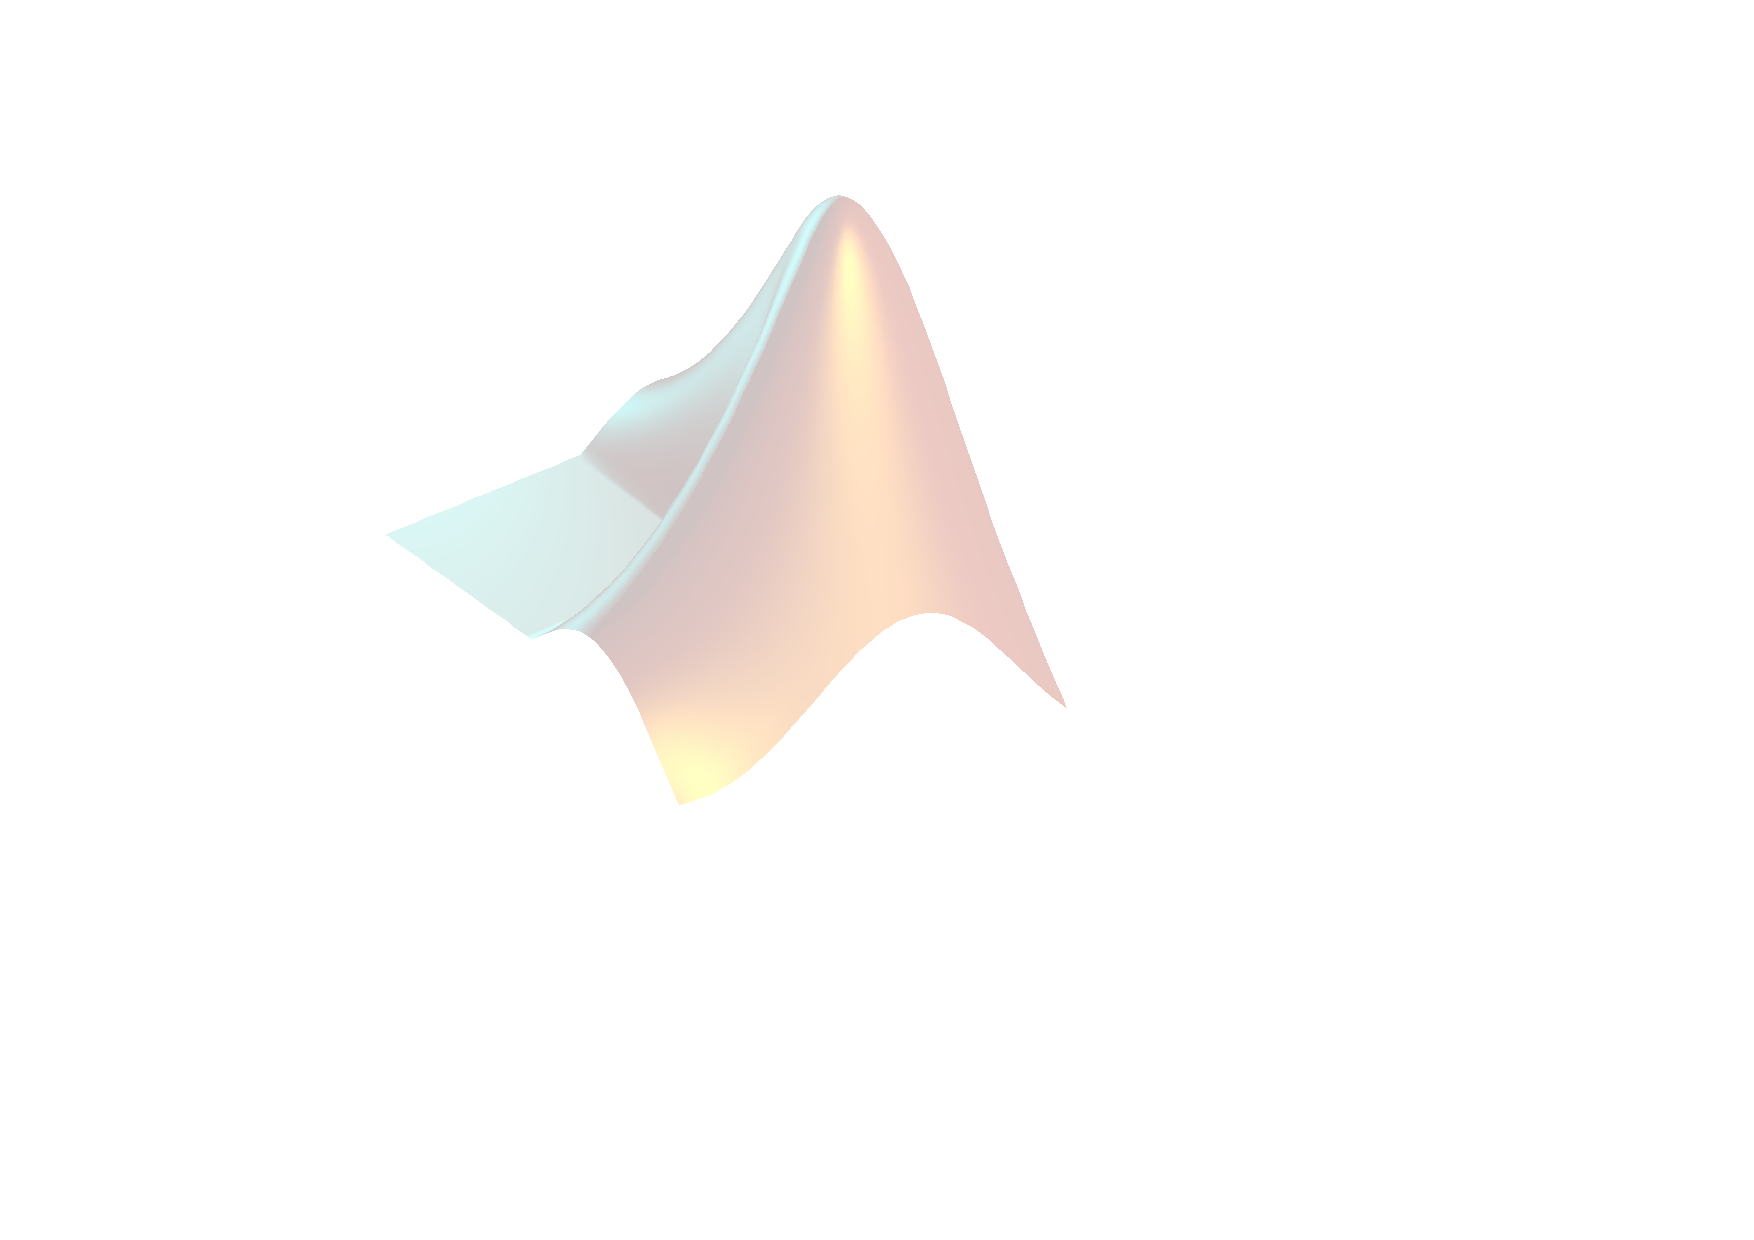
\includegraphics[width=8cm]{Graphics/General/matlab_logo_trans} \\
%            \vspace{-60mm}
            \color{Maroon}\LARGE{\textsc{an interactive introduction to}} \\ \medskip
            \color{Maroon}\Huge{\textsc{\mlab}} 
            
        \endgroup
        
		\vfill
        
        
\includegraphics[width=3cm]{Graphics/General/UoE_logo} \\   
		\myUni, \mySchool \\
	%	\myName, \textcopyright\ \myTime   
		 \textcopyright\ \myTime                  
    \end{center}
\end{titlepage}   
\cleardoublepage%*******************************************************
% About this course
%*******************************************************
\pdfbookmark[1]{About this course}{About this course}
\begingroup
\let\clearpage\relax
\let\cleardoublepage\relax
\let\cleardoublepage\relax

\chapter*{About the course}
This course was developed in the \href{http://www.eng.ed.ac.uk}{School of Engineering} at \href{http://www.ed.ac.uk}{The University of Edinburgh} to provide appropriate material for teaching \mlab \footnote{\mlab\textregistered\ is a registered trademark of MathWorks\\} in all engineering disciplines as well as to a wider audience. It is a self-study, self-paced course that emphasises responsible learning. The course material consists of this document used in conjunction with a series of video screencasts that are hosted on the School of Engineering YouTube channel.\\

\textsc{Who should use this document?}
\begin{quote}
This document is targeted at those with no prior knowledge of \mlab, and no previous programming experience. The aim, upon completion of the course, is to be competent using the most common features in \mlab and be able to apply them to solve engineering problems.
\end{quote}

\textsc{What is in this document?}
\begin{quote}
This document forms part of a self-study course to help you get started with \mlab. It should be used along with the supporting \href{https://www.youtube.com/playlist?list=PLDlE-GBjzmBZsxFKZfp6Y59qDOJVIh4RN}{video screencasts} and any additional material that maybe hosted on your institutions virtual learning environment. The main body of this document contains the fundamental topics for the course and there are also several more advanced topics given in appendices.
\end{quote}

\textsc{How to use this document?}
\begin{quote}
This document contains different elements designed to make your learning experience as smooth as possible. To benefit the most from these elements you are encouraged to use the online PDF version of this document \graffito{You can use the commenting tools in Adobe Reader to add your own notes to this PDF document}. One of the first things you'll notice is that this document contains many links, those in \textcolor{webbrown}{red} indicate a link to online material, and those in \textcolor{RoyalBlue}{blue} indicate a link to another section of this document. 

A key part of this course are the screencasts, \href{http://en.wikipedia.org/wiki/Screencast}{which are video screen captures} (http://en.wikipedia.org/wiki/Screencast). In this document screencasts are indicated by a link in a blue box with a clapperboard icon, like the example shown. 
\end{quote}
\graffito{Watching the screencasts and trying the examples for yourself will help you develop your skills in \mlab more quickly!}
\addtolength{\parindent}{-4mm}
\fcolorbox{myborderblue}{myblue}{%
\begin{minipage}{\linewidth}
\begin{minipage}{6mm}

\includegraphics[scale=0.03]{Graphics/General/screencast_icon}
\end{minipage}
\href{https://youtu.be/vtTlvq6s7a4}{\textit{Getting started}}\\
(https://youtu.be/vtTlvq6s7a4)
%\href{http://www.eng.ed.ac.uk/teaching/courses/matlab/getting-started.shtml}{\textit{Getting started}}\\
%(http://www.eng.ed.ac.uk/teaching/courses/matlab/getting-started.shtml)
\end{minipage}%
}\\
\addtolength{\parindent}{4mm}

\begin{quote}
Clicking on a link to a screencast will take you to the appropriate page on the course website where you will see the opening image to a University of Edinburgh screencast presented in the video player (Figure~\ref{fig:screencast}). Watching and learning from the screencasts are an essential part of the course and will help you develop your skills in \mlab more quickly.
\begin{figure}
	\myfloatalign
	
\includegraphics[width=\linewidth]{Graphics/General/screencast}
	\caption{A University of Edinburgh screencast}
	\label{fig:screencast}
\end{figure}

You will also notice two other types of blue box environments in this document: one is for \textit{Hints and Tips} (with a question mark icon), and the other contains exercises that you should complete (with an inkwell icon).
\end{quote}
\addtolength{\parindent}{-4mm}
\fcolorbox{myborderblue}{myblue}{%
\begin{minipage}{\linewidth}
\begin{minipage}{6mm}

\includegraphics[scale=0.03]{Graphics/General/help_icon}
\end{minipage}
\textit{Hints and Tips} \\
Throughout this document you will also see \textit{Hints and Tips} boxes like this one. Please read these as they contain \textit{useful} hints!
\end{minipage}%
}\\
\addtolength{\parindent}{4mm}\\

\addtolength{\parindent}{-4mm}
\fcolorbox{myborderblue}{myblue}{%
\begin{minipage}{\linewidth}
\begin{minipage}{6mm}
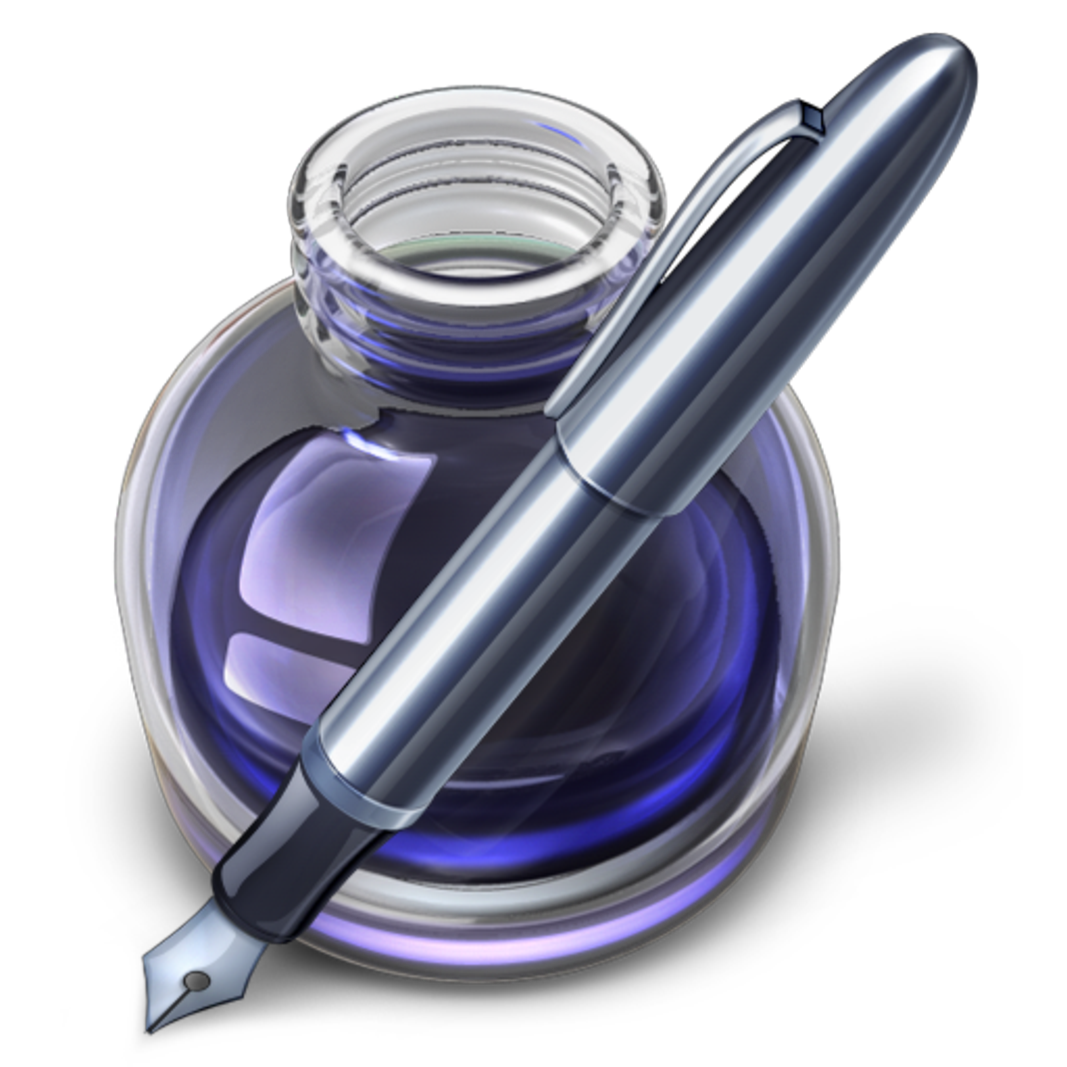
\includegraphics[scale=0.035]{Graphics/General/exercise_icon}
\end{minipage}
\textit{An example exercise}

\begin{minipage}{6mm}

\includegraphics[scale=0.03]{Graphics/General/screencast_icon}
\end{minipage}
\textit{\textcolor{webbrown}{Example exercise solutions}}
\end{minipage}%
}\\
\addtolength{\parindent}{4mm}

\begin{quote}
Additionally there are grey box environments in this document. Like the example shown (Listing~\ref{lst:lst_example}), these contain code listings that demonstrate actual \mlab code. Line numbers are given to the left of the listings to make is simpler to refer to specific bits of code. Very often you will be required to copy and paste the listing into \mlab and try running it for yourself.
\end{quote}
\begin{lstlisting}[caption={Example of a code listing},label=lst:lst_example]	 
>> 5+5
ans =
	 10
\end{lstlisting}
\vspace{5mm}

\textsc{Sources of help and further reading}
\begin{quote}
There are a huge number of textbooks published on the subject of \mlab! A user-friendly textbook that provides a good introduction to \mlab is:\graffito{Available from \href{http://www.amazon.co.uk/MATLAB-Introduction-Applications-Amos-Gilat/dp/0470108770/ref=sr_1_2?ie=UTF8&qid=1322656950&sr=8-2}{Amazon} for c.\pounds15}
\begin{itemize}
\item Gilat, A. (2008). \textit{\mlab: An Introduction With Applications}. John Wiley \& Sons, Inc., 3rd edition. 
\end{itemize}
There are a couple of further textbooks listed in the \hyperref[app:bibliography]{Bibliography} section at the end of this document. However, throughout this course and beyond, the most important source of help is the documentation built-in to \mlab. It is easily searchable, and because \mlab contains many built-in functions it is worth checking out before starting to write your own code.
\begin{itemize}
\item \mlab help documentation\\(\href{http://www.mathworks.com/access/helpdesk/help/techdoc/}{http://www.mathworks.com/access/helpdesk/help/techdoc/})\\ Accessed through the help menu in \mlab, or online.
\item \mlab \textsc{Central}\\(\href{http://www.mathworks.co.uk/matlabcentral/}{http://www.mathworks.co.uk/matlabcentral/})\\An open exchange for users, with code snippets, help forums and blogs. A great place to search for specific help!
\end{itemize}
\end{quote}

% List of books
\nocite{Pratap:2006fk} 
\nocite{Magrab:2005fk}
\nocite{Moore:2009fk}

\newpage
\textsc{Development of the course}
\begin{quote}
The development of this course was funded through The Edinburgh Fund Small Project Grant which is part of The University of Edinburgh Campaign \\ (\href{http://www.edinburghcampaign.com/alumni-giving/grants}{http://www.edinburghcampaign.com/alumni-giving/grants}).

The material for this course was developed by \href{http://www.bath.ac.uk/chem-eng/people/duren/}{Prof. Tina D\"uren}, \href{https://www.eng.ed.ac.uk/about/people/dr-antonis-giannopoulos}{Dr. Antonis Giannopoulos}, \href{Prof. Guillermo Rein}{https://www.imperial.ac.uk/people/g.rein}, \href{https://www.eng.ed.ac.uk/about/people/prof-john-thompson}{Prof. John Thompson}, and \href{https://www.northumbria.ac.uk/about-us/our-staff/w/craig-warren/}{Dr. Craig Warren}. The original screencasts were created by Dr. Craig Warren. Revised screencasts (to reflect an update to the \mlab User Interface - \mlab R2013a) were made by Joe Burchell.
\end{quote}

\textsc{License and usage of this course}
\begin{quote}
This work is licensed under the Creative Commons Attribution-NonCommercial-ShareAlike 3.0 Unported License. To view a copy of this license, visit \href{http://creativecommons.org/licenses/by-nc-sa/3.0/ <http://creativecommons.org/licenses/by-nc-sa/3.0/}{http://creativecommons.org/licenses/by-nc-sa/3.0/} or send a letter to Creative Commons, PO Box 1866, Mountain View, CA 94042, USA.

Under the terms of the license we would be grateful if you would cite the following paper:
\begin{itemize}
\item Warren, C. (2014). \mlab for Engineers: Development of an Online, Interactive, Self-study Course. Engineering Education, 9(1), 86-93. 
\end{itemize}
\end{quote}

\textsc{Acknowledgments}
\begin{quote}
An Interactive Introduction to \mlab makes use of the \href{http://www.miede.de/#classicthesis}{classicthesis template} for LaTeX, which was created by Prof. Dr.-Ing. Andr\'{e} Miede.
\end{quote}

\endgroup
\pagestyle{scrheadings}
\cleardoublepage%*******************************************************
% Table of Contents
%*******************************************************
%\phantomsection
\refstepcounter{dummy}
\pdfbookmark[1]{\contentsname}{tableofcontents}
\setcounter{tocdepth}{2}
\tableofcontents 
%\markboth{\spacedlowsmallcaps{\contentsname}}{\spacedlowsmallcaps{\contentsname}}
%*******************************************************
% work-around to have small caps also here in the headline
% will not work at this place if the TOC has more than 2 pages
% use \manualmark and then the \markboth as above
% later a modification of \automark[section]{chapter}
%*******************************************************
% List of Figures and of the Tables
%*******************************************************
\clearpage

\begingroup 
    \let\clearpage\relax
    \let\cleardoublepage\relax
    \let\cleardoublepage\relax
    %*******************************************************
    % List of Figures
    %*******************************************************    
%    %\phantomsection 
%    \refstepcounter{dummy}
%    %\addcontentsline{toc}{chapter}{\listfigurename}
%    \pdfbookmark[1]{\listfigurename}{lof}
%    \listoffigures
%
%%    \vspace*{8ex}
%    \newpage
    
    %*******************************************************
    % List of Listings
    %*******************************************************      
	%\phantomsection 
%   \refstepcounter{dummy}
%   %\addcontentsline{toc}{chapter}{\lstlistlistingname}
%   \pdfbookmark[1]{\lstlistlistingname}{lol}
%   \lstlistoflistings
%      
%    \vspace*{8ex}
%   \newpage

   %*******************************************************
   % List of Screencasts
   %*******************************************************      
   %\phantomsection 
   \refstepcounter{dummy}
   %\addcontentsline{toc}{chapter}{\lstlistlistingname}
   \pdfbookmark[1]{\listscreencastname}{los}
   \listofscreencast
   \newpage
   
   %*******************************************************
   % List of Exercises
   %*******************************************************      
   %\phantomsection 
   \refstepcounter{dummy}
   %\addcontentsline{toc}{chapter}{\lstlistlistingname}
   \pdfbookmark[1]{\listexercisesname}{loe}
   \listofexercise
   \newpage
   
    %*******************************************************
    % List of Tables
    %*******************************************************
    %\phantomsection 
    \refstepcounter{dummy}
    %\addcontentsline{toc}{chapter}{\listtablename}
    \pdfbookmark[1]{\listtablename}{lot}
    \listoftables
        
%    \vspace*{8ex}
    \newpage
       
    %*******************************************************
    % Acronyms
    %*******************************************************
%    %\phantomsection 
%    \refstepcounter{dummy}
%    \pdfbookmark[1]{Acronyms}{acronyms}
%    \markboth{\spacedlowsmallcaps{Acronyms}}{\spacedlowsmallcaps{Acronyms}}
%    \chapter*{Acronyms}
%    \begin{acronym}[UML]
%		\acro{ABC}{Absorbing Boundary Condition}
%    \end{acronym}
                  
\endgroup

\cleardoublepage
%********************************************************************
% Mainmatter
%*******************************************************
\pagenumbering{arabic}
% use \cleardoublepage here to avoid problems with pdfbookmark
\cleardoublepage
\chapter*{About MATLAB}

\section{What is \mlab?}
\mlab is produced by MathWorks, and is one of a number of commercially available software packages for numerical computing and programming. \mlab\ provides an interactive environment for algorithm development, data visualisation, data analysis, and numerical computation. \mlab, which derives its name from MATrix LABoratory, excels at matrix operations and graphics. Its main competitors are Maple, Mathematica, and Mathcad, each with their own strengths and weaknesses. 

\graffito{\mlab student version is available for around \pounds55 + VAT}\mlab is available in both commercial and academic versions with new releases binannually \eg\ R2016a (released around March 2016), and R2016b (released around September 2016). \mlab itself is the core product and is augmented by additional toolboxes, many of which have to be purchased separately. If you want to run \mlab on your own computer MathWorks offers a student version (\href{http://www.mathworks.com/academia/student_version/}{http://www.mathworks.com/academia/student\_version/}) with some of the most commonly used toolboxes for around \pounds55 +VAT. The accompanying online material, and the first version of screenshots for this document were originally based on the R2009a release of \mlab. As the \mlab user interface was substantially redeveloped by Mathworks few years later the current version of the course has been redesigned to conform to this change and is now based on the new User interface of \mlab R2013a running under Microsoft Windows. \mlab is available for other operating systems such are Mac OS X and Linux. The User Interface is very similar and the material in this course is directly applicable to versions of \mlab running under these operating systems. Finally, as the course aims to present very basic concepts of \mlab the material is widely applicable to most versions of \mlab.

\section{How is \mlab used in industry?}
\graffito{Knowing how to use \mlab is a vital skill for many engineering jobs!}The ability to use tools such as \mlab is increasingly required by employers of graduate engineers in industry. Many job adverts specifically mention knowledge of \mlab as an essential skill.

\mlab is a widely-used tool in many different fields of engineering and science. The following is a brief list of examples from Chemical, Civil, Electrical, and Mechanical Engineering:
\begin{itemize}
\item Motorsport Teams Improve Vehicle Performance with MathWorks Tools\\
(\href{http://uk.mathworks.com/company/user_stories/penske-technology-group-enables-motorsport-teams-to-improve-vehicle-performance.html}{http://uk.mathworks.com/company/user\_stories/penske-technology-group-enables-motorsport-teams-to-improve-vehicle-performance.html})
\item Bell Helicopter Develops the First Civilian Tiltrotor\\
(\href{http://www.mathworks.com/company/newsletters/news_notes/oct06/bellhelicopter.html}{http://www.mathworks.com/company/newsletters/news\_notes/oct06/bellhelicopter.html})
\item Modeling Flexible Bodies in SimMechanics and Simulink\\
(\href{http://uk.mathworks.com/company/newsletters/articles/modeling-flexible-bodies-in-simmechanics-and-simulink.html?s_tid=srchtitle}{http://uk.mathworks.com/company/newsletters/articles/modeling-flexible-bodies-in-simmechanics-and-simulink.html?s\_tid=srchtitle})
%\item Greenhouse Designed with \mlab and Simulink Revolutionizes Agriculture in Arid Coastal Regions\\
%(\href{http://www.mathworks.com/company/user_stories/userstory2347.html?by=industry}{http://www.mathworks.com/company/user\_stories/userstory2347.html?by=industry})
%\item Thames Water Aims to Reduce Leaks by More Than 25\% Using a MATLAB-Based Leak-Location System\\
%(\href{http://www.mathworks.com/company/user_stories/userstory2354.html?by=industry}{http://www.mathworks.com/company/user\_stories/userstory2354.html?by=industry})
\item Samsung UK Develops 4G Wireless Systems with Simulink\\
(\href{http://uk.mathworks.com/company/user_stories/samsung-uk-develops-4g-wireless-systems-with-simulink.html?s_tid=srchtitle}{http://uk.mathworks.com/company/user\_stories/samsung-uk-develops-4g-wireless-systems-with-simulink.html?s\_tid=srchtitle})
\item Elektrobit Testing Ltd. Develops High-Resolution Radio Channel Measuring System\\
(\href{http://uk.mathworks.com/company/user_stories/elektrobit-testing-ltd-develops-high-resolution-radio-channel-measuring-system.html?s_tid=srchtitle}{http://uk.mathworks.com/company/user\_stories/elektrobit-testing-ltd-develops-high-resolution-radio-channel-measuring-system.html?s\_tid=srchtitle})
\item Halliburton Makes Oil Exploration Safer Using MATLAB and Neural Networks\\
(\href{http://uk.mathworks.com/company/user_stories/halliburton-makes-oil-exploration-safer-using-matlab-and-neural-networks.html?s_tid=srchtitle}{http://uk.mathworks.com/company/user\_stories/halliburton-makes-oil-exploration-safer-using-matlab-and-neural-networks.html?s\_tid=srchtitle})
\end{itemize}
\chapter{Basic concepts} \label{ch:intro}

\section{\mlab in the School of Engineering, University of Edinburgh}
\mlab is currently available under Microsoft Windows and Linux operating systems in the School of Engineering Computing Labs, and also under Microsoft Windows in all of the University's Open Access Computing Labs\footnote{(\href{http://www.ed.ac.uk/information-services/computing/desktop-personal/open-access/locations}{http://www.ed.ac.uk/information-services/computing/desktop-personal/open-access/locations})}. \mlab is available to both students and staff of the University under a site license. More information on how to \href{http://www.ed.ac.uk/information-services/computing/desktop-personal/software/main-software-deals/matlab}{get access to \mlab} on your computer can be found at the Univeristy's Information Services website\footnote{(\href{http://www.ed.ac.uk/information-services/computing/desktop-personal/software/main-software-deals/matlab}{http://www.ed.ac.uk/information-services/computing/desktop-personal/software/main-software-deals/matlab})}

\section{The \mlab environment}
When you launch \mlab you are presented with the \mlab desktop (Figure~\ref{fig:matlab_desktop}) which, by default, is divided into 4 windows:
\begin{enumerate}
\item Command Window: This is the main window, and contains the command prompt (\texttt{>>}). This is where you will type all commands.
\item Command History: Displays a list of previously typed commands. The command history persists across multiple sessions and commands can be dragged into the Command Window and edited, or double-clicked to run them again.
\item Workspace: Lists all the variables you have generated in the current session. It shows the type and size of variables, and can be used to quickly plot, or inspect the values of variables.
\item Current Directory: Shows the files and folders in the current directory. The path to the current directory is listed near the top of the \mlab desktop. By default, a \mlab folder is created in your home directory, and this is where you should save your work.
\end{enumerate}
You will use and become more familiar with the different areas of the \mlab desktop as you progress through this course. \\
\begin{figure}
	\myfloatalign
	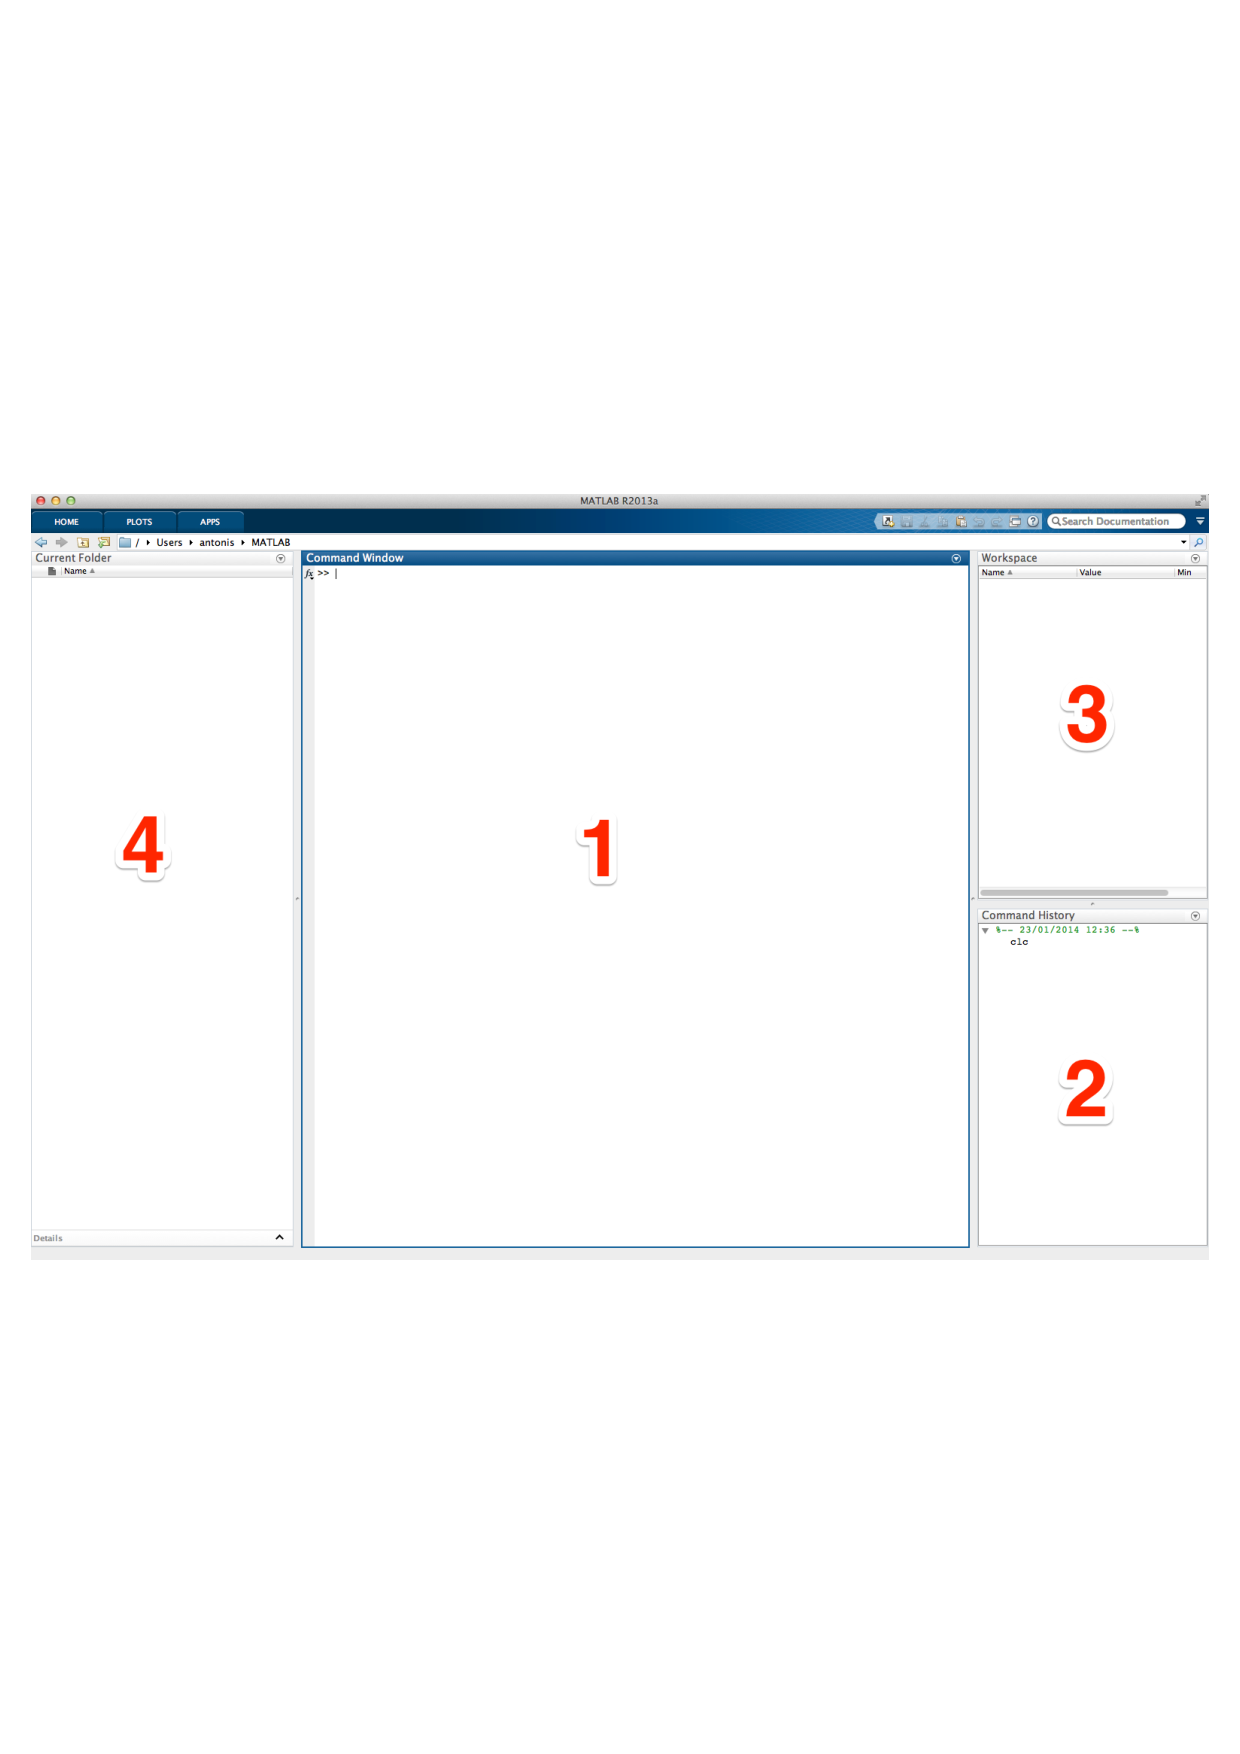
\includegraphics[width=\linewidth]{Graphics/Unit01/matlab_desktop}
	\caption{The \mlab desktop}
	\label{fig:matlab_desktop}
\end{figure}

%%%%%%%%%%%%%%%%%%%%%%%%%%%%%%%%%%%%%%%%%%%%%%
% Screencast: The MATLAB desktop
%%%%%%%%%%%%%%%%%%%%%%%%%%%%%%%%%%%%%%%%%%%%%%
\addtolength{\parindent}{-4mm}
\fcolorbox{myborderblue}{myblue}{%
\begin{minipage}{\linewidth}
\begin{minipage}{6mm}

\includegraphics[scale=0.03]{Graphics/General/screencast_icon}
\end{minipage}
\href{https://youtu.be/PfklSSxZSZU}{\screencast{The \mlab desktop}}\\
(https://youtu.be/PfklSSxZSZU)
\end{minipage}%
}\\
\addtolength{\parindent}{4mm}
\graffito{Remember you can pause the screencasts at any time and try the examples for yourself.}

\section{Basic calculations}
\mlab can perform basic calculations such as those you are used to doing on your calculator. Listings~\ref{lst:add}--\ref{lst:trig2} gives some simple examples (and results) of arithmetic operations, exponentials and logarithms, trigonometric functions, and complex numbers that can be entered in the Command Window.
\begin{lstlisting}[caption={Addition},label=lst:add]
>> 4+3
ans = 
	 7
\end{lstlisting}	 

\graffito{Try using \mlab as an expensive calculator!} 
\begin{lstlisting}[caption={Exponentiation},label=lst:exp]
>> 2^2
ans = 
	 4
\end{lstlisting}	

\begin{lstlisting}[caption={Trigonometry},label=lst:trig1]
>> sin(2*pi)+exp(-3/2)
ans = 
	 0.2231
\end{lstlisting}
\graffito{The arguments to trigonometric functions should be given in radians.}
\subsubsection{Comments:}
\begin{itemize}
\item \mlab has pre-defined constants \eg\ $\pi$ may be typed as \mcode{pi}.
\item You must explicitly type all arithmetic operations \eg\ \mcode{sin(2*pi)} not \mcode{sin(2pi)}.
\item \mcode{sin(x)} and \mcode{exp(x)} correspond to $\sin(x)$ and $e^x$ respectively.
\end{itemize}

\begin{lstlisting}[caption={Complex numbers},label=lst:complex]
>> 5+5j
ans =
	 5.0000 + 5.0000i
\end{lstlisting}

\subsubsection{Comments:}
\begin{itemize}
\item Complex numbers can be entered using the basic imaginary unit \mcode{i} or \mcode{j}.
\end{itemize}

\begin{lstlisting}[caption={More trigonometry},label=lst:trig2]	 
>> atan(5/5)
ans =
	 0.7854
	 
>> 10*log10(0.5)
ans =
	 -3.0103
\end{lstlisting}

\subsubsection{Comments:}
\begin{itemize}
\item \mcode{atan(x)} and \mcode{log10(x)} correspond to $\tan^{-1}(x)$ and $log_{10}(x)$ respectively.
\end{itemize}

\begin{table}[h]
	\caption{Arithmetic operations}
	\label{tab:arith_ops}
	\myfloatalign
	\begin{tabular}{ll}\toprule
	\spacedlowsmallcaps{Command} & \spacedlowsmallcaps{Description}\\ \midrule
	\mcode{+} & Addition \\
	\mcode{-} & Subtraction \\
	\mcode{*} & Multiplication \\
	\mcode{/} & Division \\
	\mcode{^} & Exponentiation \\
	\bottomrule
	\end{tabular}
\end{table}

\addtolength{\parindent}{-4mm}
\fcolorbox{myborderblue}{myblue}{%
\begin{minipage}{\linewidth}
\begin{minipage}{6mm}

\includegraphics[scale=0.03]{Graphics/General/help_icon}
\end{minipage}
\textit{Built-in functions} \\
There are many other built-in \mlab functions for performing basic calculations. These can be searched from the Help Browser which is opened by clicking on its icon (like the icon used to indicate this Hints and Tips section) in the \mlab desktop toolbar.
\end{minipage}%
}\\
\addtolength{\parindent}{4mm}

%%%%%%%%%%%%%%%%%%%%%%%%%%%%%%%%%%%%%%%%%%%%%%
% Exercise 1: Basic calculations
%%%%%%%%%%%%%%%%%%%%%%%%%%%%%%%%%%%%%%%%%%%%%%
\addtolength{\parindent}{-4mm}
\fcolorbox{myborderblue}{myblue}{%
\begin{minipage}{\linewidth}
\begin{minipage}{6mm}
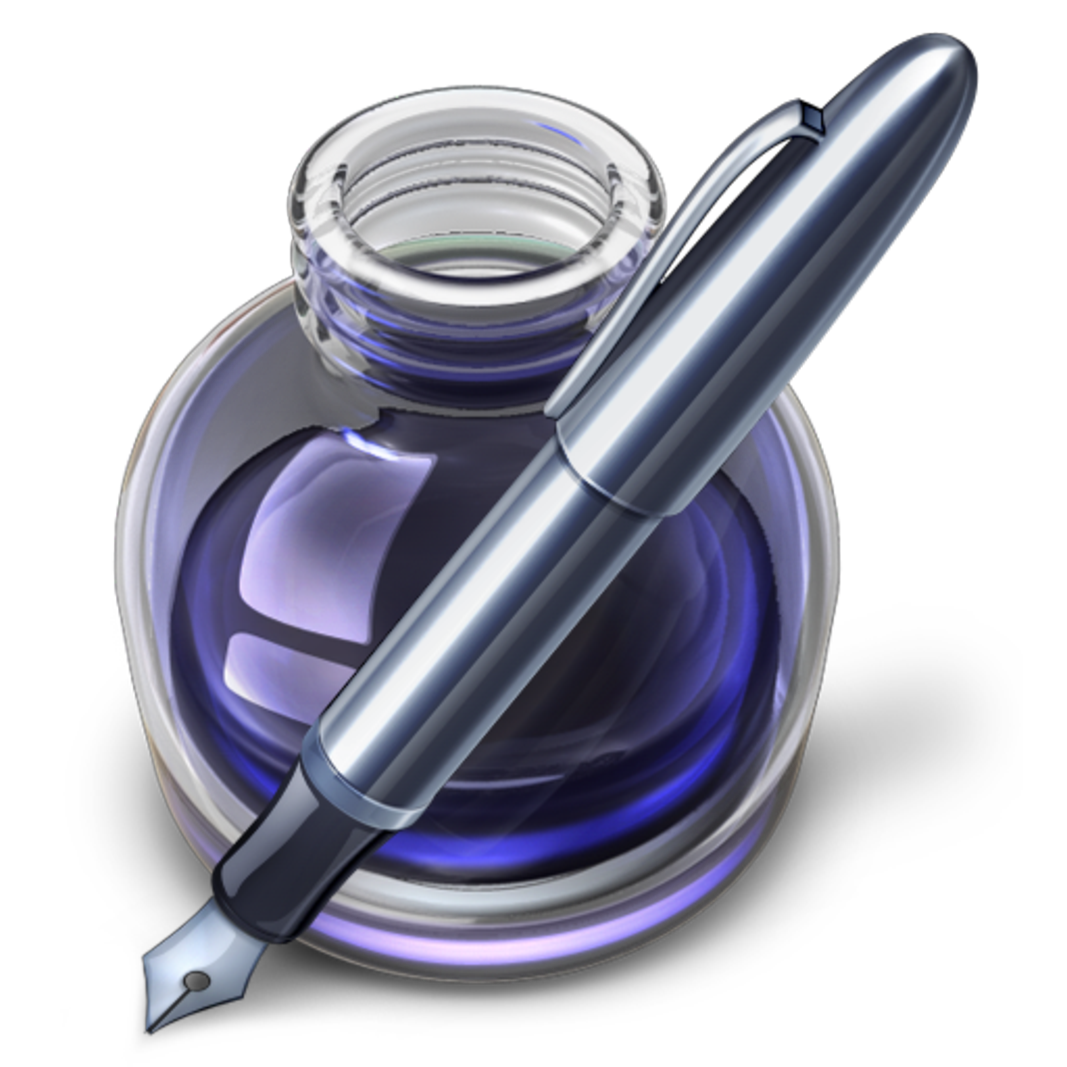
\includegraphics[scale=0.035]{Graphics/General/exercise_icon}
\end{minipage}
\exercise{\textit{Exercise 1: Basic calculations}}
\begin{enumerate}
\item Launch \mlab and explore the different areas of the \mlab desktop.
\item Try the basic calculations given in Listings~\ref{lst:add}--\ref{lst:trig2}, and check you get the correct answers.
\item \textit{Arithmetic operations} \\
Compute the following:
	\begin{itemize}
	\item $\frac{2^5}{2^5-1}$ and compare with $\left( 1-\frac{1}{2^5} \right) ^ {-1}$
	\item $\frac{\sqrt{5}-1}{(\sqrt{5}+1)^2}$
	\end{itemize}
\footnotesize{\textit{[Answers: 1.0323, 1.0323, 0.1180]}}
\normalsize
\item \textit{Exponentials and logarithms} \\
Compute the following:
	\begin{itemize}
	\item $e^3$
	\item $ln(e^3)$
	\item $log_{10}(e^3)$
	\item $log_{10}(10^5)$
	\end{itemize}
\footnotesize{\textit{[Answers: 20.0855, 3, 1.3029, 5]}}
\normalsize
\item \textit{Trigonometric operations} \\
Compute the following:
	\begin{itemize}
	\item $\sin(\frac{\pi}{6})$
	\item $\cos(\pi)$
	\item $\tan(\frac{\pi}{2})$
	\item $\sin^2(\frac{\pi}{6}) + \cos^2(\frac{\pi}{6})$
	\end{itemize}
\footnotesize{\textit{[Answers: 0.5, -1, 1.6331E16, 1]}}
\normalsize
\end{enumerate}
%%%%%%%%%%%%%%%%%%%%%%%%%%%%%%%%%%%%%%%%%%%%%%
% Screencast: Exercise 1 Solutions
%%%%%%%%%%%%%%%%%%%%%%%%%%%%%%%%%%%%%%%%%%%%%%
\begin{minipage}{6mm}

\includegraphics[scale=0.03]{Graphics/General/screencast_icon}
\end{minipage}
\href{https://youtu.be/rZuAns0iEt4}{\screencast{Exercise 1 Solutions}}\\
(https://youtu.be/rZuAns0iEt4)
%\href{http://www.eng.ed.ac.uk/teaching/courses/matlab/unit01/Ex1-Solutions.shtml}{\screencast{Exercise 1 Solutions}}\\
%(http://www.eng.ed.ac.uk/teaching/courses/matlab/unit01/Ex1-Solutions.shtml)
\end{minipage}%
}\\
\addtolength{\parindent}{4mm}

You may have noticed that the result of each of the basic calculations you performed was always assigned to a variable called \mcode{ans}. Variables are a very important concept in \mlab.

\section{Variables and arrays}
A variable is a symbolic name associated with a value. The current value of the variable is the data actually stored in the variable. Variables are very important in \mlab because they allow us to easily reference complex and changing data. Variables can reference different data types \ie\ scalars, vectors, arrays, matrices, strings \etc. Variable names must consist of a letter which can be followed by any number of letters, digits, or underscores. \mlab is case sensitive \ie\ it distinguishes between uppercase and lowercase letters \eg\ \mcode{A} and \mcode{a} are not the same variable.

Variables you have created in the current \mlab session can be viewed in a couple of different ways. The Workspace (shown in Figure~\ref{fig:matlab_desktop}) lists all the current variables and allows you to easily inspect their type and size, as well as quickly plot them. Alternatively, the \mcode{whos} command can be typed in the Command Window and provides information about the type and size of current variables. Listing~\ref{lst:whos} shows the output of the \mcode{whos} command after storing and manipulating a few variables.

\begin{lstlisting}[caption={Using the \mcode{whos} command},label=lst:whos]
>> a = 2
a = 
	 2
>> b = 3
b = 
	 3
>> c = a*b
c = 
	 6
>> edinburgh = a+5
edinburgh = 
	 7
>> whos
  Name           Size            Bytes  Class     Attributes

  a              1x1                 8  double              
  b              1x1                 8  double              
  c              1x1                 8  double              
  edinburgh      1x1                 8  double
\end{lstlisting}

Arrays are lists of numbers or expressions arranged in horizontal rows and vertical columns. A single row, or single column array is called a vector. An array with $m$ rows and $n$ columns is called a matrix of size $m \times n$. Listings~\ref{lst:row_vect}--\ref{lst:ranges} demonstrate how to create row and column vectors, and matrices in \mlab.

\begin{lstlisting}[caption={Creating a row vector},label=lst:row_vect]
>> x = [1 2 3]
x = 
	 1    2    3
\end{lstlisting}
\begin{itemize}
\item Square brackets are used to denote a vector or matrix.
\item Spaces are used to denote columns.
\end{itemize}

\begin{lstlisting}[caption={Creating a column vector},label=lst:col_vect]	
>> y = [4; 5; 6]
y = 
	 4
	 5
	 6
\end{lstlisting}
\begin{itemize}
\item The semicolon operator is used to separate columns.
\end{itemize}

\begin{lstlisting}[caption={The transpose operator},label=lst:transpose]	
>> x'
ans = 
	  1
	  2
	  3
	 
>> y'
ans =
	  4    5    6
\end{lstlisting}
\begin{itemize}
\item The single quotation mark \mcode{'} transposes arrays, i.e. the rows and columns are interchanged so that the first column becomes the first row etc...
\end{itemize}

A more efficient method for entering vectors, especially those that contain many values, is to use ranges. Instead of entering each individual value separately, a range of values can be defined as shown in Listing~\ref{lst:ranges}.
\newpage
\begin{lstlisting}[caption={Creating vectors using ranges},label=lst:ranges]	
>> z = 8:1:10
z = 
	 8    9    10
	 
>> v = linspace(0,10,5)
v =
	 0    2.5000    5.0000    7.5000    10.0000
\end{lstlisting}

\subsubsection{Comments:}
\begin{itemize}
\item A range can be created using the colon operator, \eg\ \mcode{8:1:10} means create a range that starts at 8 and goes up in steps of size 1 until 10.
\item A range can also be created using the \mcode{linspace} function, \\ \eg\ \mcode{linspace(0,10,5)} means create a range between 0 and 10 with 5 linearly spaced elements.
\end{itemize}

\addtolength{\parindent}{-4mm}
\fcolorbox{myborderblue}{myblue}{%
\begin{minipage}{\linewidth}
\begin{minipage}{6mm}

\includegraphics[scale=0.03]{Graphics/General/help_icon}
\end{minipage}
\mcode{clear} \textit{and} \mcode{clc} \textit{commands} \\
The \mcode{clear} command can be used if you want to clear the current workspace of all variables. Additionally, the \mcode{clc} command can be used to clear the Command Window, i.e. remove all text.
\end{minipage}%
}\\
\addtolength{\parindent}{4mm}
\vspace{5mm}

%%%%%%%%%%%%%%%%%%%%%%%%%%%%%%%%%%%%%%%%%%%%%%
% Screencast: Variables and simple arrays
%%%%%%%%%%%%%%%%%%%%%%%%%%%%%%%%%%%%%%%%%%%%%%
\addtolength{\parindent}{-4mm}
\fcolorbox{myborderblue}{myblue}{%
\begin{minipage}{\linewidth}
\begin{minipage}{6mm}

\includegraphics[scale=0.03]{Graphics/General/screencast_icon}
\end{minipage}
\href{https://youtu.be/Nsme7btg75U}{\screencast{Variables and simple arrays}}\\
(https://youtu.be/Nsme7btg75U)
%\href{http://www.eng.ed.ac.uk/teaching/courses/matlab/unit01/variables-arrays.shtml}{\screencast{Variables and simple arrays}}\\
%(http://www.eng.ed.ac.uk/teaching/courses/matlab/unit01/variables-arrays.shtml)
\end{minipage}%
}\\
\addtolength{\parindent}{4mm}

\mlab excels at matrix operations, and consequently the arithmetic operators such as multiplication (\mcode{*}), division (\mcode{/}), and exponentiation (\mcode{^}) perform matrix multiplication, division, and exponentiation, when used on a vector, by default. To perform an element-by-element multiplication, division, or exponentiation you must precede the operator with a dot. Table~\ref{tab:arith_ops_elemental} and Listing~\ref{lst:dot} demonstrate the dot operator.

\begin{lstlisting}[caption={The dot operator},label=lst:dot]
>> clear
>> a = [2 3; 5 1]
a = 
	 2    3
	 5    1
>> b = [4 7; 9 6]
b = 
	 4    7
	 9    6
>> a*b
ans = 
	35	 32
	29	 41
>> a.*b
ans = 
	 8    21
	45	  6
>> c = [1 2 3 4]
c = 
	 1    2    3    4
>> a*c
??? Error using ==> mtimes
Inner matrix dimensions must agree.
>> a.*c
??? Error using ==> mtimes
Matrix dimensions must agree.
\end{lstlisting}

\subsubsection{Comments:}
\begin{itemize}
\item The dot operator signifies an element-by-element operation. The dot can be used for multiplication \mcode{.*}, division \mcode{./}, or exponentiation \mcode{.^} of elements of vectors that are the same size. Omitting the dot before an arithmetic operator means \mlab performs the matrix version of the operation.
\item On Line 21 we tried to perform a matrix multiplication of a 2$\times$2 matrix with a 1$\times$4 matrix. This results in an error because you can only multiply two matrices if the number of columns in the first equals the number of rows in the second.
\item On Line 24 we get a similar error if we try to perform an element-by-element multiplication, as this does not make any sense for matrices of different sizes.
\end{itemize}

\begin{table}[h]
	\caption{Element-by-element arithmetic operations}
	\label{tab:arith_ops_elemental}
	\myfloatalign
	\begin{tabular}{ll}\toprule
	\spacedlowsmallcaps{Command} & \spacedlowsmallcaps{Description}\\ \midrule
	\mcode{.*} & Element-by-element multiplication \\
	\mcode{./} & Element-by-element division \\
	\mcode{.^} & Element-by-element exponentiation \\
	\bottomrule
	\end{tabular}
\end{table}

%%%%%%%%%%%%%%%%%%%%%%%%%%%%%%%%%%%%%%%%%%%%%%
% Screencast: The dot operator
%%%%%%%%%%%%%%%%%%%%%%%%%%%%%%%%%%%%%%%%%%%%%%
\addtolength{\parindent}{-4mm}
\fcolorbox{myborderblue}{myblue}{%
\begin{minipage}{\linewidth}
\begin{minipage}{6mm}

\includegraphics[scale=0.03]{Graphics/General/screencast_icon}
\end{minipage}
\href{https://youtu.be/gvxxr2R0S-o}{\screencast{The dot operator}}\\
(https://youtu.be/gvxxr2R0S-o)
%\href{http://www.eng.ed.ac.uk/teaching/courses/matlab/unit01/dot-operator.shtml}{\screencast{The dot operator}}\\
%(http://www.eng.ed.ac.uk/teaching/courses/matlab/unit01/dot-operator.shtml)
\end{minipage}%
}\\
\addtolength{\parindent}{4mm}
\vspace{5mm}

\addtolength{\parindent}{-4mm}
\fcolorbox{myborderblue}{myblue}{%
\begin{minipage}{\linewidth}
\begin{minipage}{6mm}

\includegraphics[scale=0.03]{Graphics/General/help_icon}
\end{minipage}
\textit{Read \mlab error messages!}\\
\textcolor{red}{\mcode{??? Error using ==> mtimes} \\
\mcode{Inner matrix dimensions must agree.}} \\
This error message example usually indicates you tried to perform a matrix operation when you intended an element-by-element operation. You should check your code for a missing dot operator.
\end{minipage}%
}\\
\addtolength{\parindent}{4mm}

You can access individual elements, entire rows and columns, and subsets of matrices using the notation \mcode{matrix_name(row,column)}. Listing~\ref{lst:access_matrices} demonstrates how to access elements in a matrix. \graffito{Square brackets \mcode{[ ]} are used when creating vectors, arrays and matrices, and round brackets \mcode{( )} when accessing elements in them.}
\begin{lstlisting}[caption={Accessing elements of matrices},label=lst:access_matrices]
>> w = [1 2 3 4; 5 6 7 8; 9 10 11 12]
w =
	 1    2    3    4
	 5    6    7    8
	 9   10   11   12
	 
>> size(w)
ans =
	 3    4

>> w(1,1)
ans = 
	 1
	 
>> w(3,1)
ans =
	 9
	 
>> w(3,:)
ans = 
	 9    10    11    12
	 
>> w(2,4) = 13
w =
	 1    2    3    4
	 5    6    7   13
	 9   10   11   12
	 
>> v = w(1:2,2:3)
v =
	 2    3
	 6    7
	 
>> z = w([2,3],[2,4])
z =
	 6   13
	10   12
\end{lstlisting}

\subsubsection{Comments:}
\begin{itemize}
\item On Line~7 the \mcode{size} command returns the number of rows and columns in the matrix. 
\item On Lines~11, 15 and 19, when accessing an individual element in a matrix, the first number after the round bracket refers to the row number (row index), and second number refers to the column number (column index).
\item On Line 19 the colon operator is used to denote all of the columns, i.e. all the columns in the third row are selected. The colon operator can also be used as a row index to denote all rows.
\item Line~23 demonstrates accessing a single element in the matrix \mcode{w} to change its value.
\item On Line~29 a new matrix \mcode{v} is created as a sub-matrix of \mcode{w}.
\item Finally, on Line~34 a new matrix \mcode{z} is created as a sub-matrix of \mcode{w}. Square brackets are used within the round brackets to enclose the list of row and column numbers.
\end{itemize}

%%%%%%%%%%%%%%%%%%%%%%%%%%%%%%%%%%%%%%%%%%%%%%
% Screencast: Indexing arrays
%%%%%%%%%%%%%%%%%%%%%%%%%%%%%%%%%%%%%%%%%%%%%%
\addtolength{\parindent}{-4mm}
\fcolorbox{myborderblue}{myblue}{%
\begin{minipage}{\linewidth}
\begin{minipage}{6mm}

\includegraphics[scale=0.03]{Graphics/General/screencast_icon}
\end{minipage}
\href{https://youtu.be/eEhwnCq0_Qg}{\screencast{Indexing arrays}}\\
(https://youtu.be/eEhwnCq0\_Qg)
%\href{http://www.eng.ed.ac.uk/teaching/courses/matlab/unit01/indexing-arrays.shtml}{\screencast{Indexing arrays}}\\
%(http://www.eng.ed.ac.uk/teaching/courses/matlab/unit01/indexing-arrays.shtml)
\end{minipage}%
}\\
\addtolength{\parindent}{4mm}
\vspace{5mm}

%%%%%%%%%%%%%%%%%%%%%%%%%%%%%%%%%%%%%%%%%%%%%%
% Self Test Exercise: Indexing arrays
%%%%%%%%%%%%%%%%%%%%%%%%%%%%%%%%%%%%%%%%%%%%%%
\addtolength{\parindent}{-4mm}
\begin{minipage}{\linewidth}
\begin{minipage}{6mm}
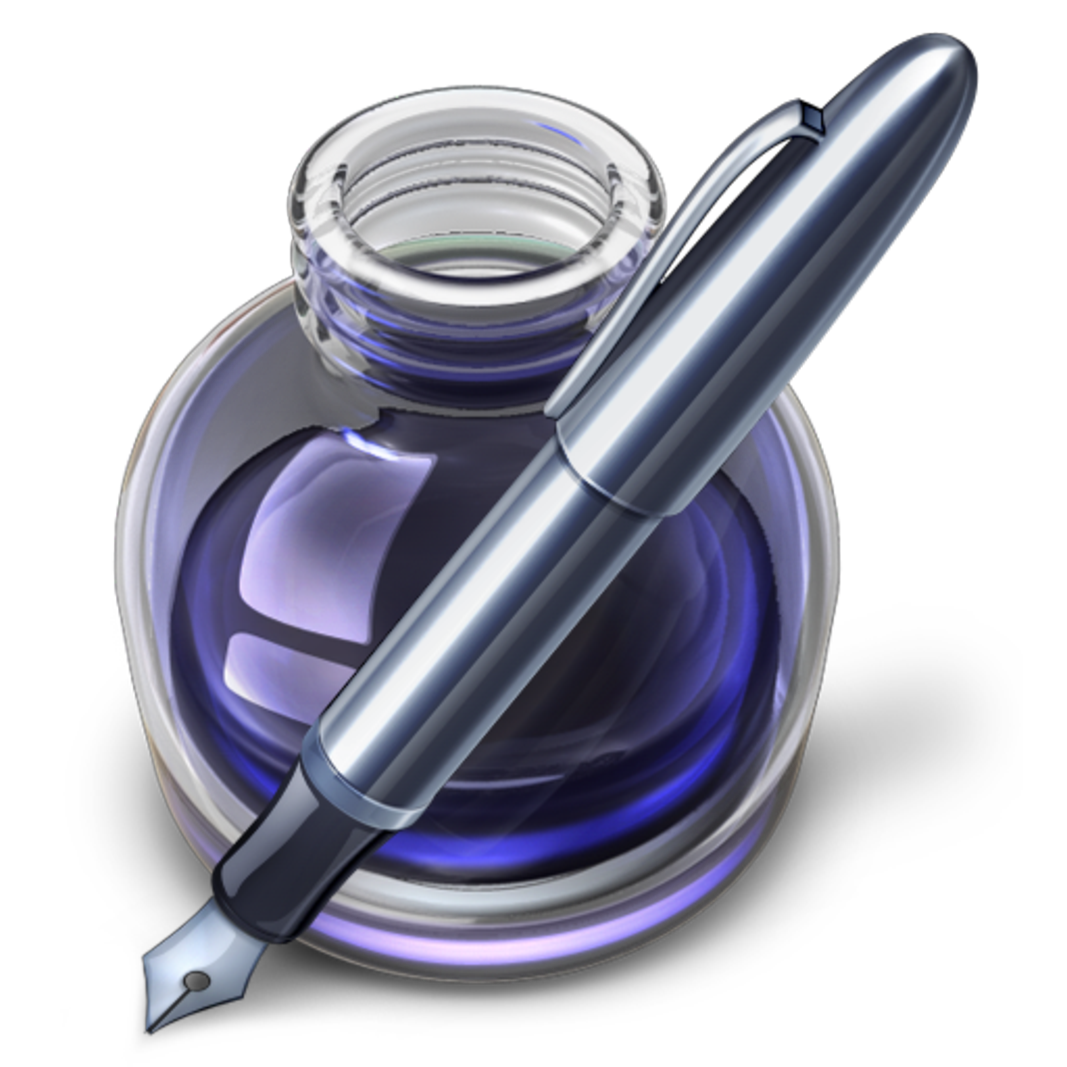
\includegraphics[scale=0.035]{Graphics/General/exercise_icon}
\end{minipage}
\textit{Self Test Exercise: Indexing arrays}
\end{minipage}
\addtolength{\parindent}{4mm}
\begin{enumerate}
\item \footnote[2]{Question adapted from \gilatbook}The following matrix is defined:
\begin{equation*}
M=\left[ \begin{array}{rrrrrrr} 6 & 9 & 12 & 15 & 18 & 21 \\ 4 & 4 & 4 & 4 & 4 & 4 \\ 2 & 1 & 0 & -1 & -2 & -3 \\ -6 & -4 & -2 & 0 & 2 & 4 \end{array} \right]
\end{equation*}
Evaluate the following expressions without using \mlab. Check your answers with \mlab.
\begin{enumerate}
\item \mcode{A = M([1,3], [2,4])}
\item \mcode{B = M(:, [1,4:6])}
\item \mcode{C = M([2,3], :)}
\end{enumerate}
\end{enumerate}

\section{Solving systems of linear equations}
Solving systems of linear equations is one of the most common computations in science and engineering, and is easily handled by \mlab. Consider the following set of linear equations.
\begin{equation*}
\begin{split}
5x = 3y - 2z + 10 \\
8y + 4z = 3x + 20\\
2x + 4y -9z = 9
\end{split}
\end{equation*}
This set of equations can be re-arranged so that all the unknown quantities are on the left-hand side and the known quantities are on the right-hand side.
\begin{equation*}
\begin{split}
5x - 3y + 2z &= 10 \\
-3x + 8y + 4z &= 20 \\
2x + 4y - 9z &= 9
\end{split}
\end{equation*}
This is now of the form $AX=B$, where $A$ is a matrix of the coefficients of the unknowns,
\begin{equation*}
A=\left[ \begin{array}{rrr} 5 & -3 & 2 \\ -3 & 8 & 4 \\ 2 & 4 & -9 \end{array} \right]
\end{equation*}
$x$ is the vector of unknowns,
\begin{equation*}
X=\left[ \begin{array}{c} x \\ y \\ z \end{array} \right]
\end{equation*}
and $B$ is a vector containing the constants.
\begin{equation*}
B=\left[ \begin{array}{c} 10 \\ 20 \\ 9 \end{array} \right]
\end{equation*}
Listing~\ref{lst:linear_eqns1} shows the code used to solve the system of linear equations in \mlab. The rules of matrix algebra apply i.e. the result of multiplying a $N \times N$ matrix by a $N \times 1$ vector, is a $N \times 1$ vector.
\newpage
\begin{lstlisting}[caption={Solving a system of linear equations},label=lst:linear_eqns1]
>> A = [5 -3 2; -3 8 4; 2 4 -9];
>> B = [10; 20; 9;];
>> X = A\B
X = 
	3.4442
	3.1982
	1.1868
\end{lstlisting}
\graffito{Using a semi-colon at the end of a command prevents the results being displayed in the Command Window.}
\subsubsection{Comments:}
\begin{itemize}
\item On Line~1 the matrix, $A$, of coefficients of the unknowns is entered. 
\item On Line~2 the vector, $B$, containing the constants is entered. 
\item On Line~3 the vector, $X$, containing the unknowns, is calculated by using the matrix left divide operator to divide $A$ by $B$.
\end{itemize}

Listing~\ref{lst:linear_eqns2} demonstrates how to check the solution obtained in Listing~\ref{lst:linear_eqns1}.
\begin{lstlisting}[caption={Checking the solution of a system of linear equations},label=lst:linear_eqns2]
>> C = A*X
C =
	10.0000
	20.0000
	 9.0000
\end{lstlisting}
Not all systems of linear equations have a unique solution. If there are fewer equations than variables, the problem is under-specified. If there are more equations than variables, it is over-specified.

\vspace{5mm}
\addtolength{\parindent}{-4mm}
\fcolorbox{myborderblue}{myblue}{%
\begin{minipage}{\linewidth}
\begin{minipage}{6mm}

\includegraphics[scale=0.03]{Graphics/General/help_icon}
\end{minipage}
\textit{The left division or backslash operator ($\backslash$)}\\
In \mlab the left division or backslash operator ($\backslash$) is used to solve equations of the form $AX=B$ i.e. \mcode{X = A\\B}. Gaussian elimination is used to perform this operation. 
\end{minipage}%
}\\
\addtolength{\parindent}{4mm}

%%%%%%%%%%%%%%%%%%%%%%%%%%%%%%%%%%%%%%%%%%%%%%
% Exercise 2: Variables and arrays
%%%%%%%%%%%%%%%%%%%%%%%%%%%%%%%%%%%%%%%%%%%%%%
\addtolength{\parindent}{-4mm}
\fcolorbox{myborderblue}{myblue}{%
\begin{minipage}{\linewidth}
\begin{minipage}{6mm}
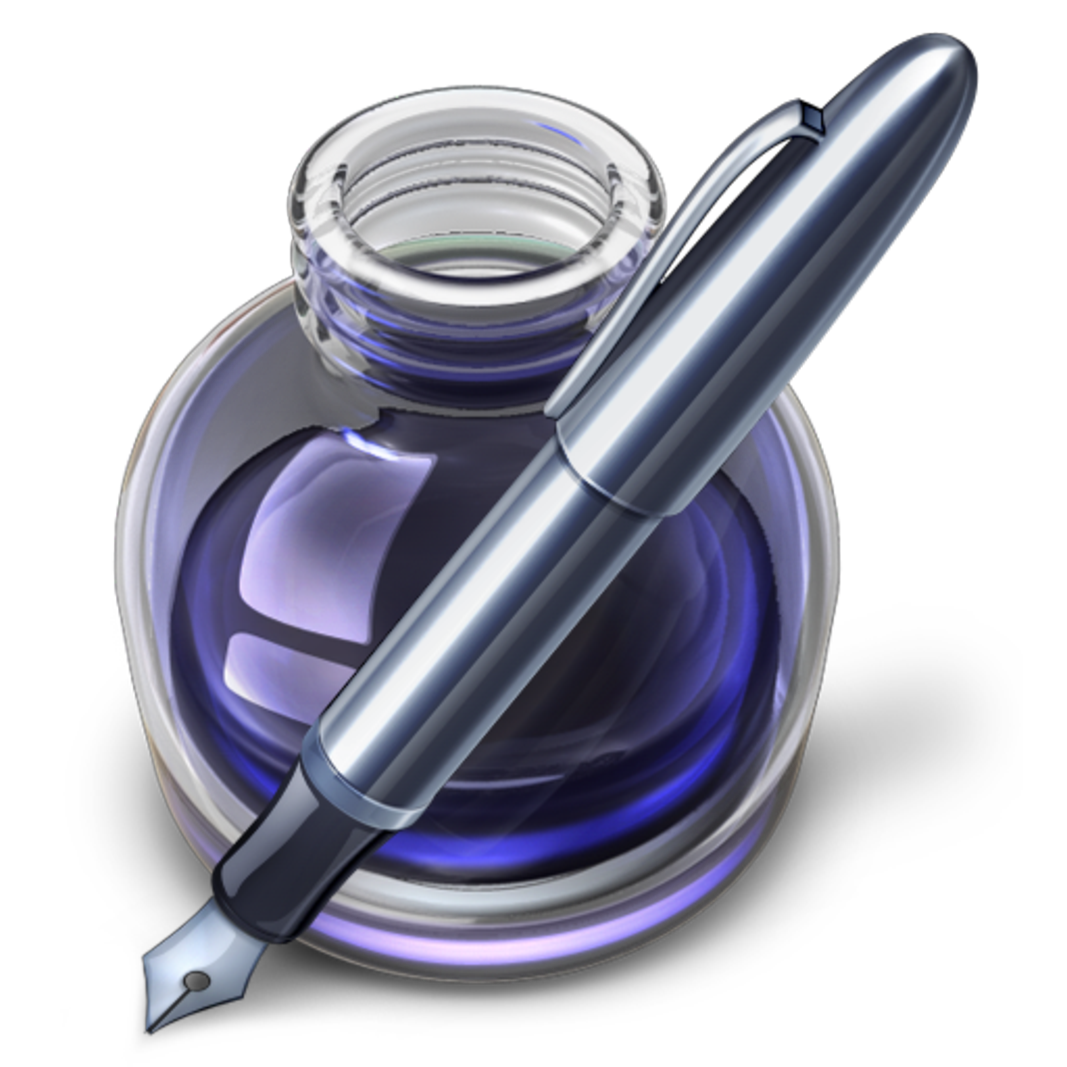
\includegraphics[scale=0.03]{Graphics/General/exercise_icon}
\end{minipage}
\exercise{\textit{Exercise 2: Variables and arrays}}
\begin{enumerate}
\item Create the variables to represent the following matrices:
\begin{equation*}
A=\left[ \begin{array}{cccc} 12 & 17 & 3 & 4 \end{array} \right] \qquad
B=\left[ \begin{array}{ccc} 5 & 8 & 3 \\ 1 & 2 & 3 \\ 2 & 4 & 6 \end{array} \right] \qquad
C=\left[ \begin{array}{c} 22 \\ 17 \\ 4 \end{array} \right]
\end{equation*}
	\begin{enumerate}
	\item Assign to the variable \mcode{x1} the value of the second column of matrix \mcode{A}.
	\item Assign to the variable \mcode{x2} the third column of matrix \mcode{B}.
	\item Assign to the variable \mcode{x3} the third row of matrix \mcode{B}.
	\item Assign to the variable \mcode{x4} the first three values of matrix \mcode{A} as the first row, and all the values in matrix \mcode{B} as the second, third and fourth rows.
	\end{enumerate}

\item If matrix \mcode{A} is defined using the \mlab code \mcode{A = [1 3 2; 2 1 1; 3 2 3]}, which command will produce the following matrix? 
\begin{align*}
B&=\left[ \begin{array}{cc} 3 & 2 \\ 2 & 1 \end{array} \right]
\end{align*}

\item Create variables to represent the following matrices:
\begin{equation*}
A=\left[ \begin{array}{ccc} 1 & 2 & 3 \\ 2 & 2 & 2 \\ -1 & 2 & 1 \end{array} \right] \qquad
B=\left[ \begin{array}{ccc} 1 & 0 & 0 \\ 1 & 1 & 0 \\ 1 & 1 & 1 \end{array} \right] \qquad
C=\left[ \begin{array}{cc} 1 & 1 \\ 2 & 1 \\ 1 & 2 \end{array} \right]
\end{equation*}
	\begin{enumerate}
	\item Try performing the following operations: \mcode{A+B}, \mcode{A*B}, \mcode{A+C}, \mcode{B*A}, \mcode{B-A}, \mcode{A*C}, \mcode{C-B}, \mcode{C*A}. What are the results? What error messages are generated? Why?
	\item What is the difference between \mcode{A*B} and \mcode{A.*B}?
	\end{enumerate}

\item Solve the following systems of linear equations. Remember to verify your solutions.
\begin{enumerate}
\item \begin{equation*}
\begin{split}
-2x + y &= 3 \\
x + y &= 10
\end{split}
\end{equation*}
\end{enumerate}
\end{enumerate}
\end{minipage}%
}\\
\addtolength{\parindent}{4mm}

%%%%%%%%%%%%%%%%%%%%%%%%%%%%%%%%%%%%%%%%%%%%%%
% Exercise 2: Variables and arrays (continued)
%%%%%%%%%%%%%%%%%%%%%%%%%%%%%%%%%%%%%%%%%%%%%%
\addtolength{\parindent}{-4mm}
\fcolorbox{myborderblue}{myblue}{%
\begin{minipage}{\linewidth}
\begin{minipage}{6mm}
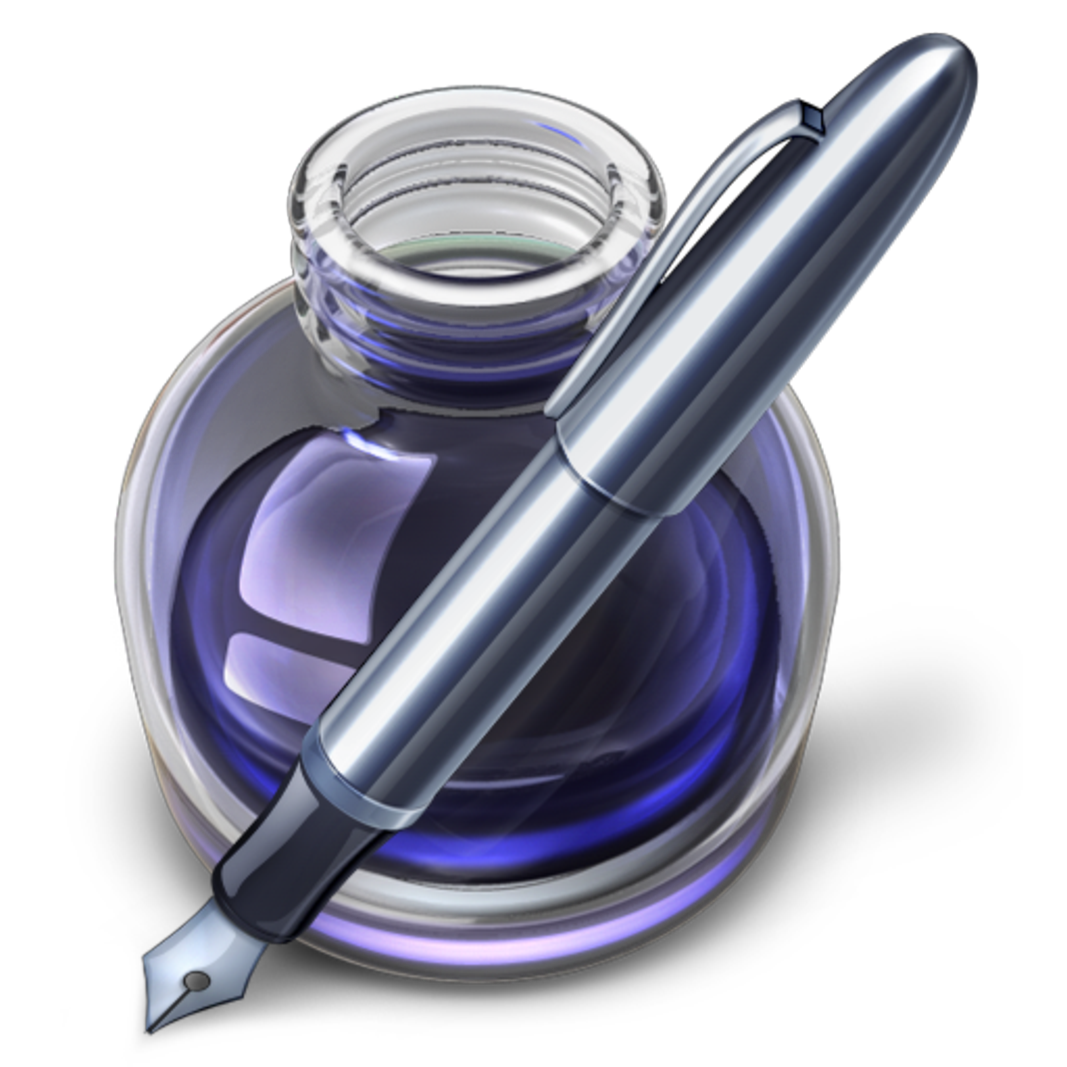
\includegraphics[scale=0.035]{Graphics/General/exercise_icon}
\end{minipage}
\textit{Exercise 2: Variables and arrays (continued)}
\begin{enumerate}
\setcounter{enumi}{3}
\item \textit{continued}
\begin{enumerate}
\setcounter{enumii}{1}
\item \begin{equation*}
\begin{split}
5x + 3y -z &= 10 \\
3x + 2y + z &= 4 \\
4x - y + 3z &= 12
\end{split}
\end{equation*}
\item \begin{equation*}
\begin{split}
x_1 - 2x_2 - x_3 + 3x_4 &= 10 \\
2x_1 + 3x_2 + x_4 &= 8 \\
x_1 - 4x_3 - 2x_4 &= 3 \\
-x_2 + 3x_3 + x_4 &= -7
\end{split}
\end{equation*}
\end{enumerate}

\item Create a vector \mcode{t} that ranges from 1 to 10 in steps of 1, and a vector \mcode{theta} that ranges from 0 to $\pi$ and contains 32 elements. Now compute the following: 
\begin{align*}
x&=2sin(\theta) \\
y&=\frac{t-1}{t+1} \\
z&=\frac{\sin(\theta^2)}{\theta^2}
\end{align*}

\item A discharge factor is a ratio which compares the mass flow rate at the end of a channel or nozzle to an ideal channel or nozzle. The discharge factor for flow through an open channel of parabolic cross-section is:
\begin{equation*}
K=\frac{1.2}{x}\left[ \sqrt{16x^2+1} + \frac{1}{4x} \ln \left( \sqrt{16x^2+1} + 4x \right) \right] ^{-\frac{2}{3}},
\end{equation*}
where $x$ is the ratio of the maximum water depth to breadth of the channel at the top of the water. Determine the discharge factors for $x$ in the range 0.45 to 0.90 in steps of 0.05.

\item \textit{Points on a circle} \\
All points with coordinates $x=rcos(\theta)$ and $y=rsin(\theta)$, where $r$ is a constant, lie on a circle with radius $r$, \ie\ they satisfy the equation $x^2+y^2=r^2$. Create a column vector for $\theta$ with the values $0$, $\pi/4$, $\pi/2$, $3\pi/4$, $\pi$, and $5\pi/4$. Take $r=2$ and compute the column vectors $x$ and $y$. Now check that $x$ and $y$ indeed satisfy the equation of a circle, by computing the radius $r=\sqrt{(x^2+y^2)}$.
\end{enumerate}
\end{minipage}%
}\\
\addtolength{\parindent}{4mm}

%%%%%%%%%%%%%%%%%%%%%%%%%%%%%%%%%%%%%%%%%%%%%%
% Exercise 2: Variables and arrays (continued)
%%%%%%%%%%%%%%%%%%%%%%%%%%%%%%%%%%%%%%%%%%%%%%
\addtolength{\parindent}{-4mm}
\fcolorbox{myborderblue}{myblue}{%
\begin{minipage}{\linewidth}
\begin{minipage}{6mm}
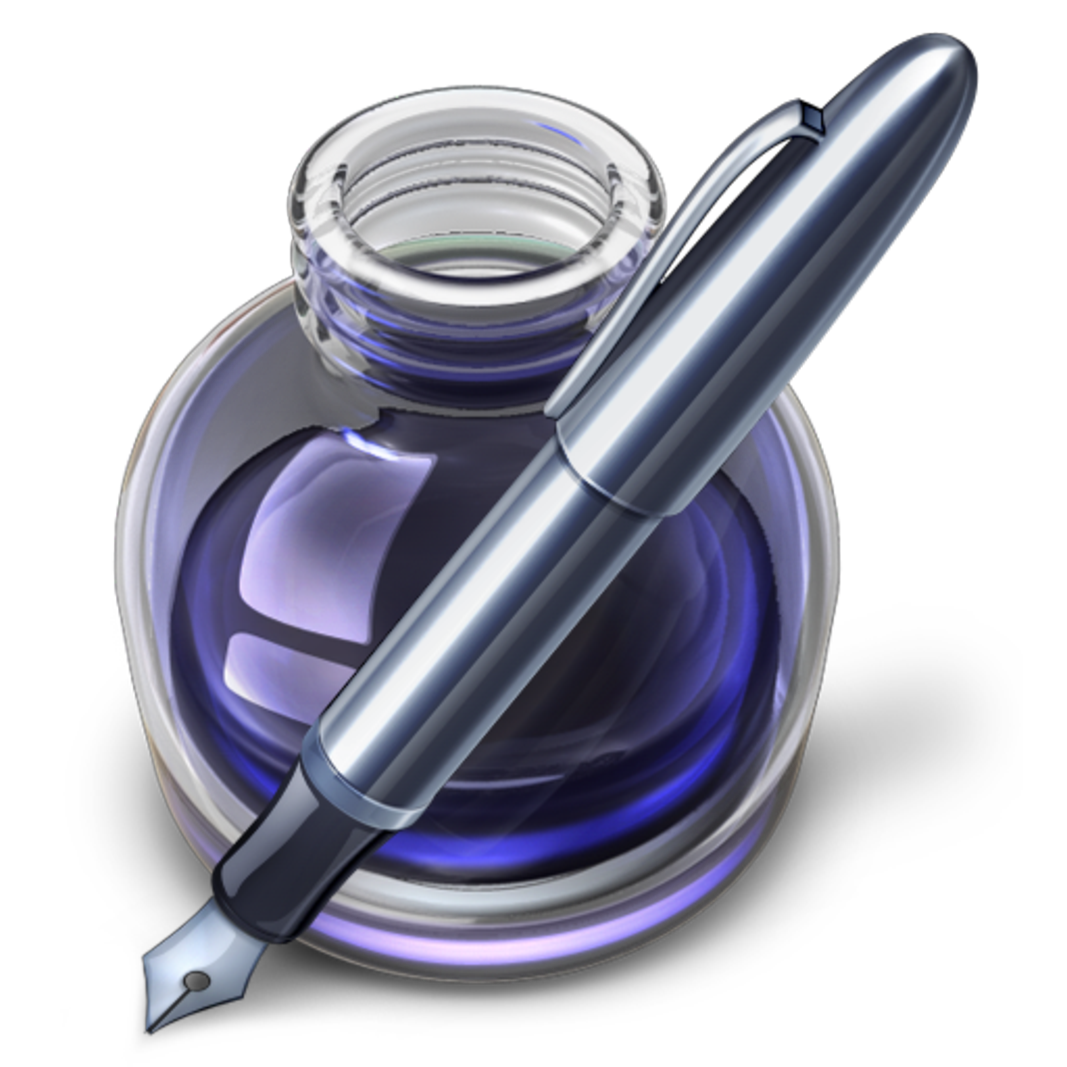
\includegraphics[scale=0.035]{Graphics/General/exercise_icon}
\end{minipage}
\textit{Exercise 2: Variables and arrays (continued)}
\begin{enumerate}
\setcounter{enumi}{7}
\item \textit{Geometric series} \\
The sum of a geometric series $1+r+r^2+r^3+\ldots+r^n$ approaches the limit $\frac{1}{1-r}$ for $r<1$ as $n\rightarrow \infty$. Take $r=0.5$ and compute sums of series 0 to 10, 0 to 50, and 0 to 100. Calculate the aforementioned limit and compare with your summations. Do the summation using the built-in \mcode{sum} function.
\end{enumerate}
%%%%%%%%%%%%%%%%%%%%%%%%%%%%%%%%%%%%%%%%%%%%%%
% Screencast: Exercise 2 Solutions
%%%%%%%%%%%%%%%%%%%%%%%%%%%%%%%%%%%%%%%%%%%%%%
\begin{minipage}{6mm}

\includegraphics[scale=0.03]{Graphics/General/screencast_icon}
\end{minipage}
\href{https://youtu.be/pTdkD1UpGjU}{\screencast{Exercise 2 Solutions Q 1 - 4}}\\
(https://youtu.be/pTdkD1UpGjU)\\
%\href{http://www.eng.ed.ac.uk/teaching/courses/matlab/unit01/Ex2-Solutions.shtml}{\screencast{Exercise 2 Solutions}}\\
%(http://www.eng.ed.ac.uk/teaching/courses/matlab/unit01/Ex2-Solutions.shtml)\\
\begin{minipage}{6mm}

\includegraphics[scale=0.03]{Graphics/General/screencast_icon}
\end{minipage}
\href{https://youtu.be/nHroWoJApT8}{\screencast{Exercise 2 Solutions Q 5 - 8}}\\
(https://youtu.be/nHroWoJApT8)\\
\end{minipage}%
}\\
\addtolength{\parindent}{4mm}

\vspace{5mm}
%%%%%%%%%%%%%%%%%%%%%%%%%%%%%%%%%%%%%%%%%%%%%%
% Reference to additional exercises
%%%%%%%%%%%%%%%%%%%%%%%%%%%%%%%%%%%%%%%%%%%%%%
\addtolength{\parindent}{-4mm}
\fcolorbox{myborderblue}{myblue}{%
\begin{minipage}{\linewidth}
\begin{minipage}{6mm}
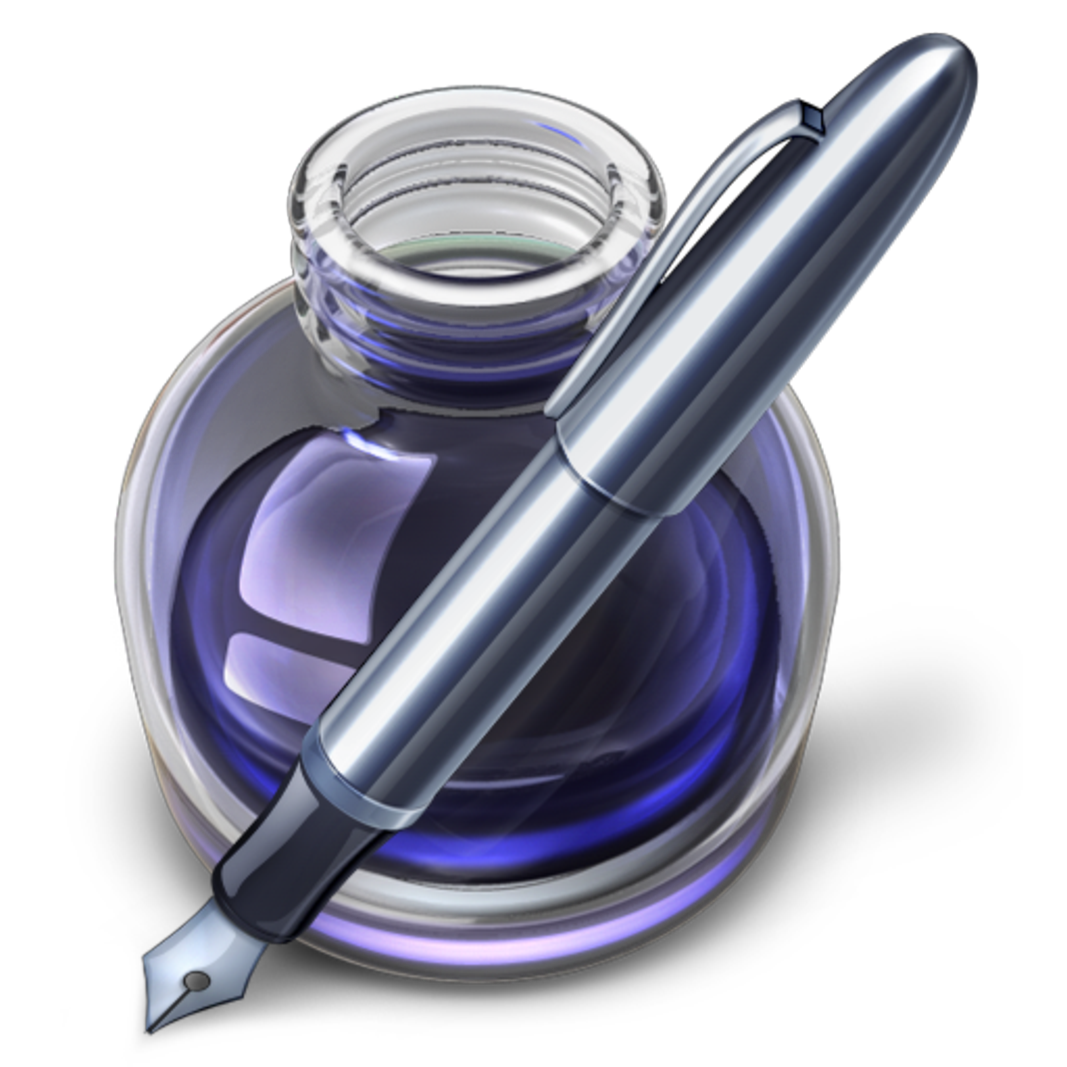
\includegraphics[scale=0.035]{Graphics/General/exercise_icon}
\end{minipage}
\textit{Additional Exercises}\\
You should now attempt questions from Chapter~\ref{sect:basic_concepts}. 
\end{minipage}%
}\\
\addtolength{\parindent}{4mm}

\chapter{Plotting}

\mlab is very powerful for producing both \twod and \threed plots. Plots can be created and manipulated interactively or by commands. \mlab offers a number of different formats for exporting plots, including EPS (Encapsulated PostScript), PDF (Portable Document Format) and JPEG (Joint Photographic Experts Group), so you can easily include \mlab plots in your reports.

\section{Simple \twod plotting}
The simplest and most commonly used plotting command is \mcode{plot(x,y)}, where \mcode{x} and \mcode{y} are simply vectors containing the $x$ and $y$ coordinates of the data to be plotted. Listing~\ref{lst:simple_plot} demonstrates the commands used to create a plot of the function, $f(x) = e^{-\frac{x}{10}} \sin(x)$, which is shown in Figure~\ref{fig:simple_plot}.
\begin{lstlisting}[caption={A simple plot},label=lst:simple_plot]
>> x = 0:0.1:20;
>> y = exp(-x/10).*sin(x);
>> plot(x,y), grid on, xlabel('x'), ...
ylabel('f(x) = e^{-x/10} sin(x)'), title('A simple plot')
\end{lstlisting}
\begin{figure}
	\myfloatalign
	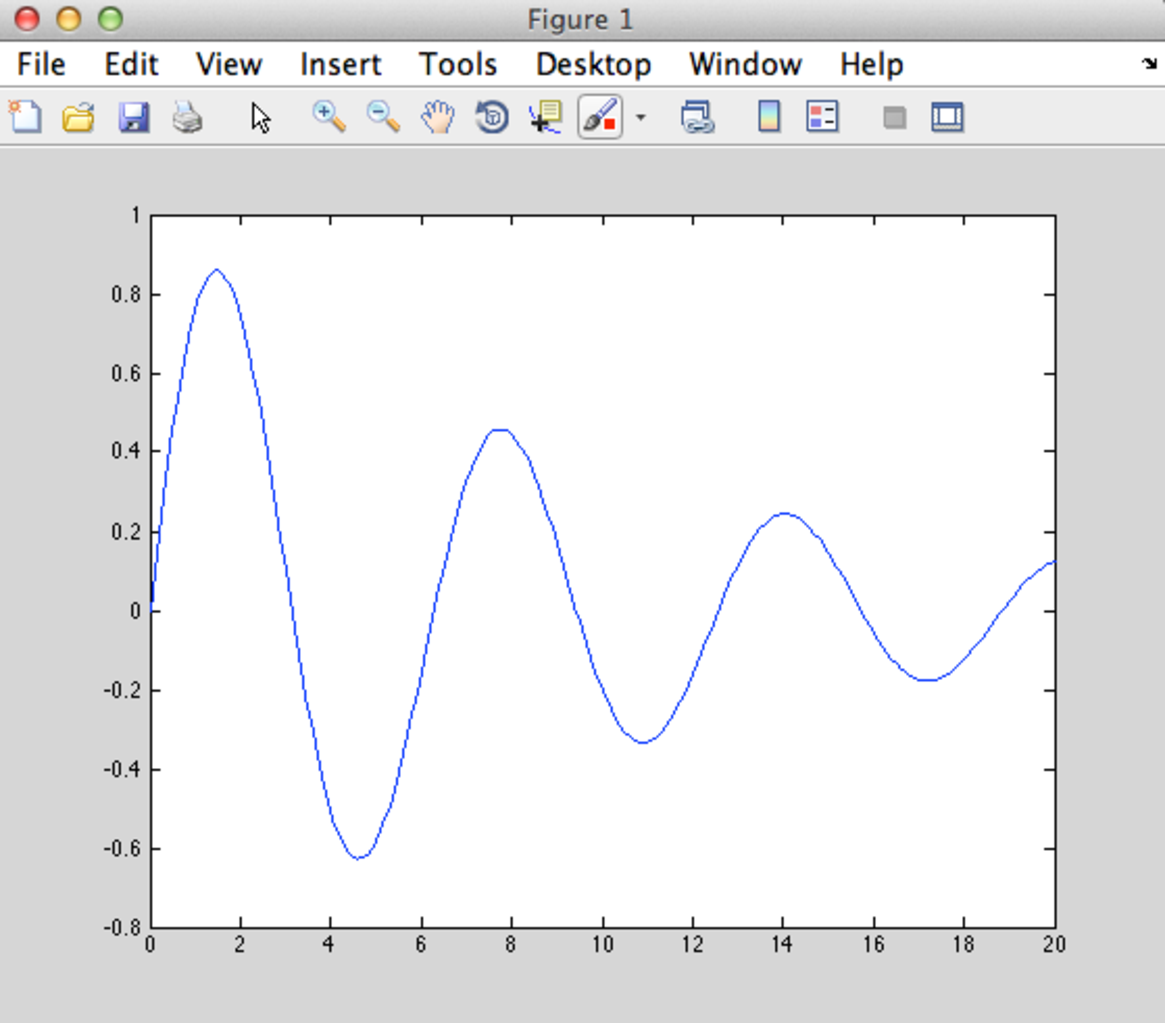
\includegraphics[width=0.9\linewidth]{Graphics/Unit02/simple_plot}
	\caption{Plot of $f(x) = e^{-\frac{x}{10}} \sin(x)$}
	\label{fig:simple_plot}
\end{figure}

\subsubsection{Comments:}
\begin{itemize}
\item The vectors containing the \mcode{x} and \mcode{y} data must be the same length.
\item The plot command can be used to plot multiple sets of data on the same axes, \ie\ \mcode{plot(x1,y1,x2,y2)}.
\item The dot-dot-dot \mcode{...} (ellipsis) notation is used to indicate that Lines 3 and 4 are one long line. The ellipsis notation just allows the line to be broken to make it more readable. Each comma-separated command could also have been typed on a separate line. 
\end{itemize}
When \mlab executes a plotting command, a new Figure Window opens with the plot in it. The following list gives the most common commands for changing plot properties.
\begin{itemize}
\item \mcode{grid on} displays the grid!
\item \mcode{xlabel('My x-axis label')}, \mcode{ylabel('My y-axis label')}, and \mcode{title('My title')} can be used to label the corresponding parts of the plot. You must enclose your labels with single quotes which denotes a string of text.
\item \mcode{legend('Data1','Data2')} is used to place a legend and label the data-sets when you have multiple data-sets on one plot.
\item You can specify line style and colour within the \mcode{plot} command \eg\ \mcode{plot(x1,y1,'b-',x2,y2,'r--')}. This command would make the first data-set a solid blue line, and the second data-set a dashed red line. Tables~\ref{tab:plot_line_styles}--\ref{tab:plot_colours} gives some of the most common line styles and colours.
\end{itemize}

\begin{table}[h]
	\caption{Line styles in plots}
	\label{tab:plot_line_styles}
	\myfloatalign
	\begin{tabular}{ll}\toprule
	\spacedlowsmallcaps{String specifier} & \spacedlowsmallcaps{Line style}\\ \midrule
	\mcode{-} & Solid line (default) \\
	\mcode{--} & Dashed line \\
	\mcode{:} & Dotted line \\
	\mcode{-.} & Dash-dot line \\
	\bottomrule
	\end{tabular}
\end{table}

\begin{table}[h]
	\caption{Colours in plots}
	\label{tab:plot_colours}
	\myfloatalign
	\begin{tabular}{ll}\toprule
	\spacedlowsmallcaps{String specifier} & \spacedlowsmallcaps{Line colour}\\ \midrule
	\mcode{r} & Red \\
	\mcode{g} & Green \\
	\mcode{b} & Blue (default) \\
	\mcode{w} & White \\
	\mcode{k} & Black \\
	\bottomrule
	\end{tabular}
\end{table}

Plot properties can also be manipulated interactively (without having to issue commands) by clicking on the \textit{Show Plot Tools} icon in the Figure Window toolbar, shown in Figure~\ref{fig:interact_icon}. Properties such as the axis limits, gridlines, line style, colour and thickness, text font type and size, and legend \etc\ can all be adjusted be clicking on the appropriate parts of the plot. \\
\begin{figure}[h]
	\myfloatalign
	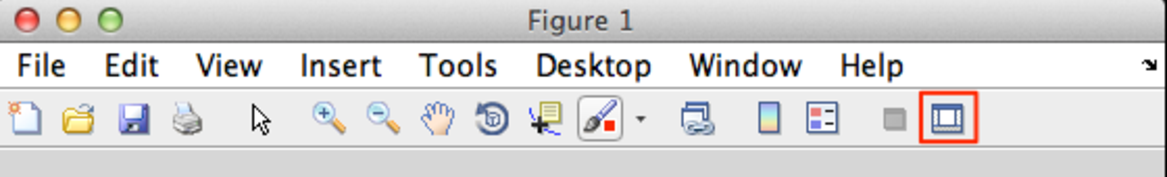
\includegraphics[width=0.9\linewidth]{Graphics/Unit02/interact_icon}
	\caption{\textit{Show Plot Tools} toolbar icon in Figure Window}
	\label{fig:interact_icon}
\end{figure}

\addtolength{\parindent}{-4mm}
\fcolorbox{myborderblue}{myblue}{%
\begin{minipage}{\linewidth}
\begin{minipage}{6mm}

\includegraphics[scale=0.03]{Graphics/General/help_icon}
\end{minipage}
\textit{Producing good plots} \\
Whether you manipulate your plots via commands or interactively, here is some useful advice for producing good plots in \mlab.
\begin{itemize}
\item Give your plot an informative title \\ \eg\ \mcode{title('Stress vs. strain of steel')}
\item Label your axes and remember to include units where appropriate \\ \eg\ \mcode{xlabel('Strain'), ylabel('Stress (MPa)')}
\item Use line colours and styles carefully so that multiple data-sets can be easily distinguished \eg\ \mcode{plot(x1,y1,'b-',x2,y2,'r--'), grid on}
\item Remember to insert a legend when you are plotting multiple data-sets on one plot \eg\ \mcode{legend('Carbon steel','Stainless steel')}
\end{itemize}
\end{minipage}%
}\\
\addtolength{\parindent}{4mm}
\vspace{5mm}

%%%%%%%%%%%%%%%%%%%%%%%%%%%%%%%%%%%%%%%%%%%%%%
% Screencast: Creating a simple plot
%%%%%%%%%%%%%%%%%%%%%%%%%%%%%%%%%%%%%%%%%%%%%%
\addtolength{\parindent}{-4mm}
\fcolorbox{myborderblue}{myblue}{%
\begin{minipage}{\linewidth}
\begin{minipage}{6mm}

\includegraphics[scale=0.03]{Graphics/General/screencast_icon}
\end{minipage}
\href{http://www.eng.ed.ac.uk/teaching/courses/matlab/unit02/simple-plot.shtml}{\screencast{Creating a simple plot}}\\
(http://www.eng.ed.ac.uk/teaching/courses/matlab/unit02/simple-plot.shtml)
\end{minipage}%
}\\
\addtolength{\parindent}{4mm}

\mlab has many built-in plot types, and a great way of getting a quick overview of all the different plot types is to select a variable in your Workspace Browser, click on the disclosure triangle next to the \textit{plot} toolbar icon and select \textit{More plots...}, as shown in Figure~\ref{fig:access_plot_catalog}. This will launch the \textit{Plot Catalog} shown in Figure~\ref{fig:plot_catalog}.
\begin{figure}[h]
	\myfloatalign
	\subfloat[Accessing the \textit{Plot Catalog}]
	%%%% Changed width from 0.45 AG 23/01/2014 %%%%
    {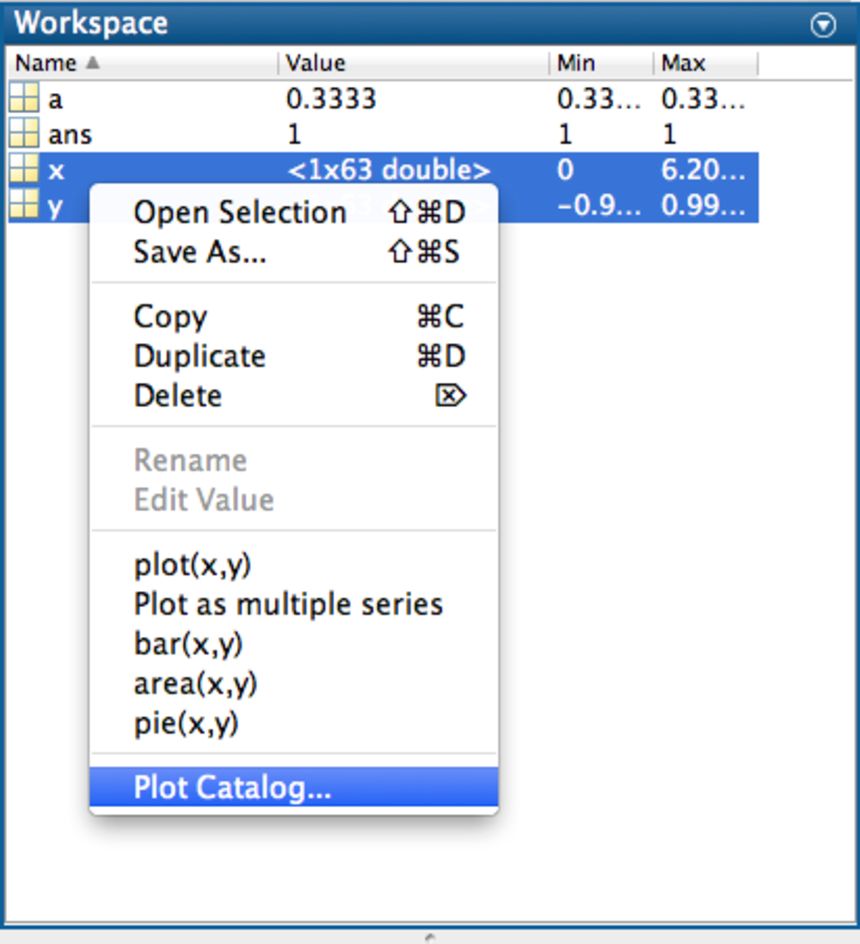
\includegraphics[width=0.45\linewidth]{Graphics/Unit02/access_plot_catalog}\label{fig:access_plot_catalog}} \\
    \subfloat[The \textit{Plot Catalog}]
    {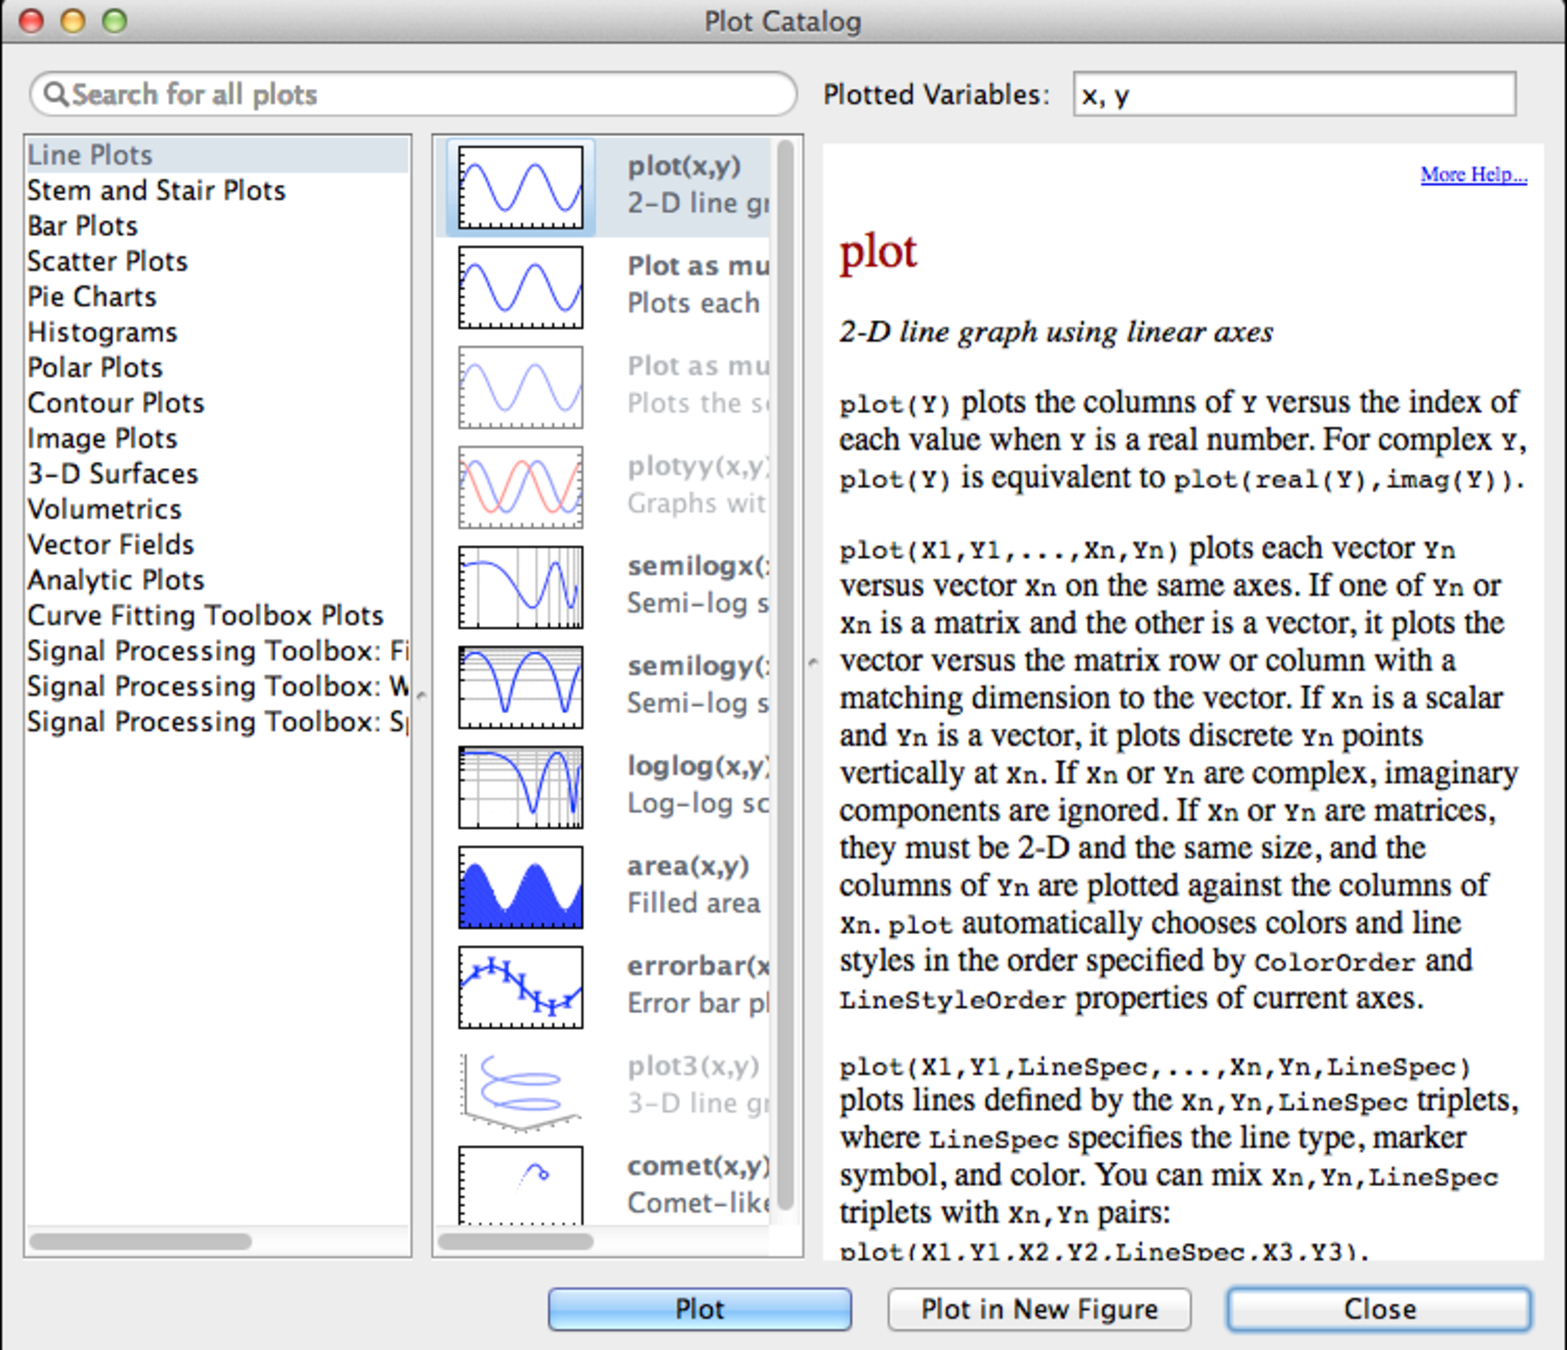
\includegraphics[width=\linewidth]{Graphics/Unit02/plot_catalog}\label{fig:plot_catalog}}
    \caption{\textit{The Plot Catalog}}
\end{figure}

%%%%%%%%%%%%%%%%%%%%%%%%%%%%%%%%%%%%%%%%%%%%%%
% Screencast: Plotting experimental data
%%%%%%%%%%%%%%%%%%%%%%%%%%%%%%%%%%%%%%%%%%%%%%
\addtolength{\parindent}{-4mm}
\fcolorbox{myborderblue}{myblue}{%
\begin{minipage}{\linewidth}
\begin{minipage}{6mm}

\includegraphics[scale=0.03]{Graphics/General/screencast_icon}
\end{minipage}
\href{http://www.eng.ed.ac.uk/teaching/courses/matlab/unit02/plot-exp-data.shtml}{\screencast{Plotting experimental data}}\\
(http://www.eng.ed.ac.uk/teaching/courses/matlab/unit02/plot-exp-data.shtml)
\end{minipage}%
}\\
\addtolength{\parindent}{4mm}
\vspace{5mm}

\addtolength{\parindent}{-4mm}
\fcolorbox{myborderblue}{myblue}{%
\begin{minipage}{\linewidth}
\begin{minipage}{6mm}

\includegraphics[scale=0.03]{Graphics/General/help_icon}
\end{minipage}
\textit{Importing data from external sources} \\
You can import data from other programs into \mlab using the \textit{Copy \textrightarrow Paste} method, or using the \textit{Import Data Wizard}, found at \textit{File \textrightarrow Import Data...}, for Microsoft Excel data, Comma-separated value files and more. There are also functions, \mcode{xlsread} and \mcode{xlswrite}.
\end{minipage}%
}\\
\addtolength{\parindent}{4mm}

\subsection{Multiple plots in one Figure Window}
The \mcode{subplot} command can be used to display a number of different plots in a single Figure Window, as shown in Figure~\ref{fig:subplots}. The \mcode{subplot} command takes three arguments that determine the number and location of plots in the Figure Window. For example, \mcode{subplot(2,2,1)} specifies that the Figure Window will be divided into 2 rows and 2 columns of plots, and selects the first subplot to plot into. Listing~\ref{lst:subplots} shows an example of usage of the \mcode{subplot} command.
\begin{lstlisting}[caption={Using the \mcode{subplot} command},label=lst:subplots]
>> x = linspace(0,2*pi,50);
>> subplot(2,2,1), plot(x,sin(x)), xlabel('x'), ylabel('sin(x)');
>> subplot(2,2,2), plot(x,cos(x)), xlabel('x'), ylabel('cos(x)');
>> subplot(2,2,3), plot(x,sin(2*x)), xlabel('x'), ylabel('sin(2x)');
>> subplot(2,2,4), plot(x,cos(2*x)), xlabel('x'), ylabel('cos(2x)');
\end{lstlisting}
\begin{figure}[h]
	\myfloatalign
	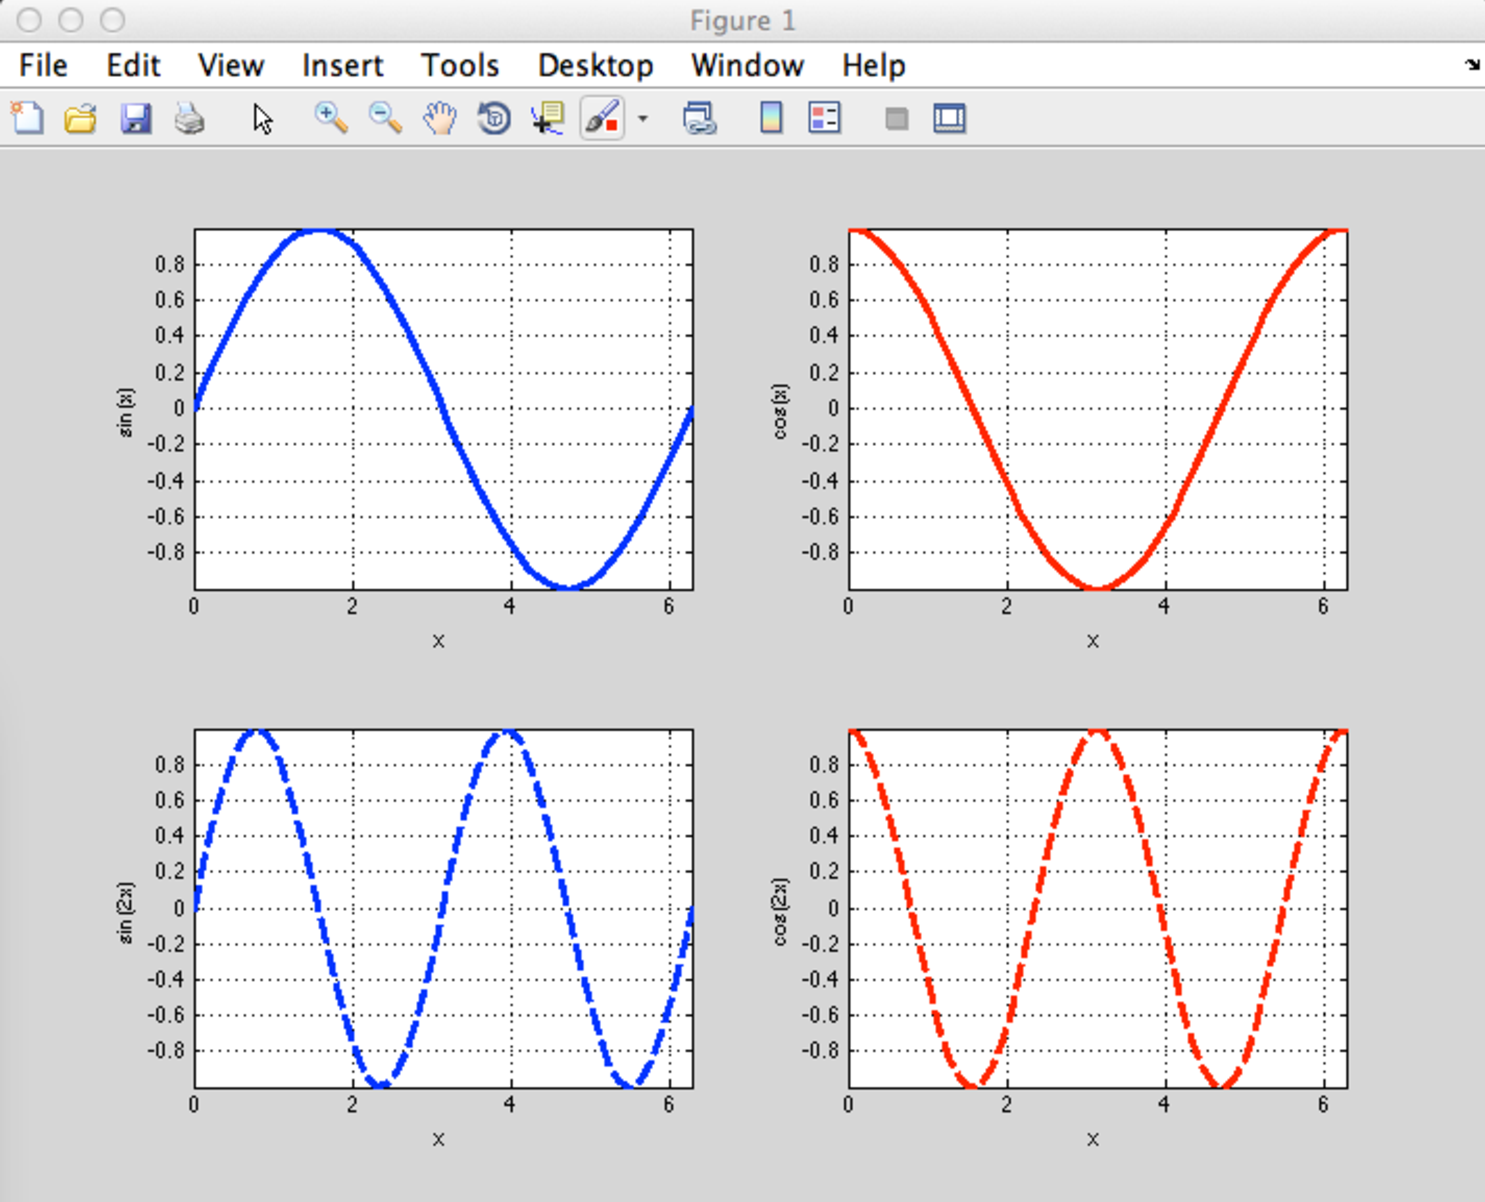
\includegraphics[width=0.9\linewidth]{Graphics/Unit02/subplots}
	\caption{Example of subplots}
	\label{fig:subplots}
\end{figure}

\newpage
%%%%%%%%%%%%%%%%%%%%%%%%%%%%%%%%%%%%%%%%%%%%%%
% Exercise 3: Simple 2D plotting
%%%%%%%%%%%%%%%%%%%%%%%%%%%%%%%%%%%%%%%%%%%%%%
\addtolength{\parindent}{-4mm}
\fcolorbox{myborderblue}{myblue}{%
\begin{minipage}{\linewidth}
\begin{minipage}{6mm}
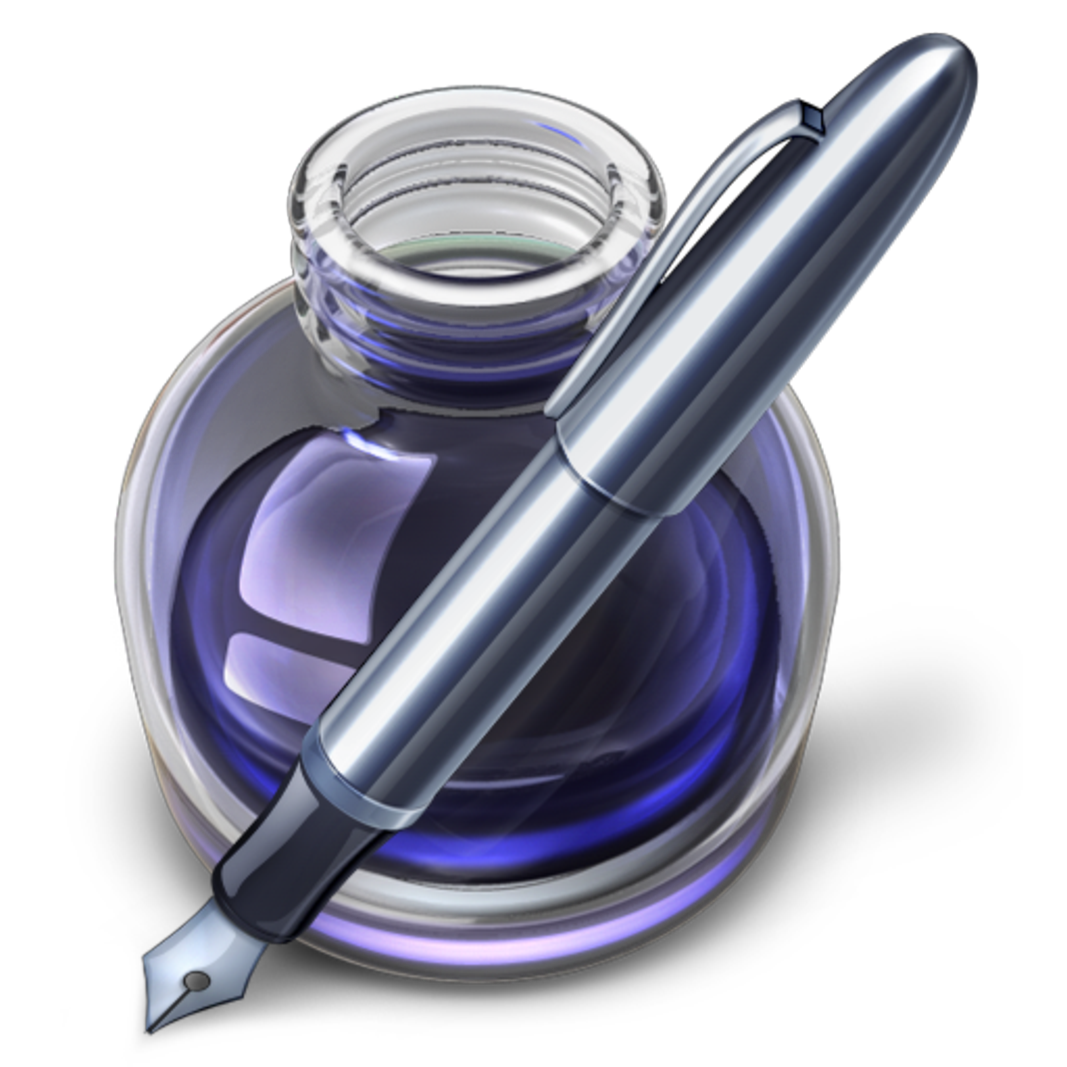
\includegraphics[scale=0.035]{Graphics/General/exercise_icon}
\end{minipage}
\exercise{\textit{Exercise 3: Simple \twod plotting}} \\
Please save all the plots you produce using the \textit{File \textrightarrow Save} option in the Figure Window. This should save a file with the \mlab default Figure format which uses a \textit{.fig} file extension.
\begin{enumerate}
\item Plot the following functions (you will need to decide on appropriate ranges for $x$):
	\begin{itemize}
	\item $y=\frac{1}{x}$, with a blue dashed line.
	\item $y=\sin(x)\cos(x)$, with a red dotted line.
	\item $y=2x^2-3x+1$, with red cross markers. 
	\end{itemize}
	Turn the \mcode{grid on} in all your plots, and remember to label axes and use a title.
\item Given the following function: \\
\begin{equation*}
s=a \cos(\phi) + \sqrt{b^2 - (a \sin(\phi) - c)^2}
\end{equation*}
Plot $s$ as a function of angle $\phi$ when $a=1$, $b=1.5$, $c=0.3$, and $0 \leq \phi \leq 360^\circ$.
\item Plot the following parametric functions (you will need to use the \mcode{axis equal} command after your \mcode{plot} command to force \mlab to make the x-axis and y-axis the same length):
	\begin{enumerate}
	\item A circle of radius 5 (revisit Ex2 Q7)
	\item \textit{Leminscate} $(-\pi/4 \leq \phi \leq \pi/4)$
		\begin{align*}
		x &= \cos(\phi)\sqrt{2cos(2\phi)} \\
		y &= \sin(\phi)\sqrt{2cos(2\phi)}
		\end{align*}
	\item \textit{Logarithmic Spiral} $(0 \leq \phi \leq 6\pi; k=0.1)$
		\begin{align*}
		x &= e^{k\phi}\cos(\phi) \\
		y &= e^{k\phi}\sin(\phi)
		\end{align*}
	\end{enumerate}
\end{enumerate}
%%%%%%%%%%%%%%%%%%%%%%%%%%%%%%%%%%%%%%%%%%%%%%
% Screencast: Exercise 3 Solutions
%%%%%%%%%%%%%%%%%%%%%%%%%%%%%%%%%%%%%%%%%%%%%%
\begin{minipage}{6mm}

\includegraphics[scale=0.03]{Graphics/General/screencast_icon}
\end{minipage}
\href{http://www.eng.ed.ac.uk/teaching/courses/matlab/unit02/Ex3-Solutions.shtml}{\screencast{Exercise 3 Solutions}}\\
(http://www.eng.ed.ac.uk/teaching/courses/matlab/unit02/Ex3-Solutions.shtml)
\end{minipage}%
}\\
\addtolength{\parindent}{4mm}

\section{Curve-fitting}
\mlab provides a number of powerful options for fitting curves and adding trend-lines to data. The Basic Fitting Graphical User Interface (GUI) can be selected from Figure Windows by selecting \textit{Basic fitting} from the \textit{Tools} menu, and offers common curve-fitting options for \twod plots. More advanced functionality, including \threed fits, can be accessed from the Curve Fitting Toolbox using tools such as \mcode{cftool} (for curve fitting) and \mcode{sftool} (for surface fitting)\footnote{Only basic curve-fitting will be covered in this course.}. \\

%%%%%%%%%%%%%%%%%%%%%%%%%%%%%%%%%%%%%%%%%%%%%%
% Screencast: Basic Curve-fitting
%%%%%%%%%%%%%%%%%%%%%%%%%%%%%%%%%%%%%%%%%%%%%%
\addtolength{\parindent}{-4mm}
\fcolorbox{myborderblue}{myblue}{%
\begin{minipage}{\linewidth}
\begin{minipage}{6mm}

\includegraphics[scale=0.03]{Graphics/General/screencast_icon}
\end{minipage}
\href{http://www.eng.ed.ac.uk/teaching/courses/matlab/unit02/basic-curve-fitting.shtml}{\screencast{Basic Curve-fitting}}\\
(http://www.eng.ed.ac.uk/teaching/courses/matlab/unit02/basic-curve-fitting.shtml)
\end{minipage}%
}\\
\addtolength{\parindent}{4mm}

An alternative to the Basic Fitting GUI are the functions \mcode{polyfit} and \mcode{polyval} which can be used to do basic curve-fitting programmatically. Listing~\ref{lst:polyfit} demonstrates how \mcode{polyfit} can be used to fit a polynomial to a data-set.
\begin{lstlisting}[caption={Syntax of \mcode{polyfit} command},label=lst:polyfit]
coeff = polyfit(xdata,ydata,n);
\end{lstlisting}

\subsubsection{Comments:}
\begin{itemize}
\item \mcode{coeff} is a vector containing the coefficients for the polynomial of best fit, \mcode{xdata} and \mcode{ydata} are vectors containing the independent and dependent variables, and \mcode{n} denotes the degree of the polynomial to be fitted.
\end{itemize}
After using \mcode{polyfit} you can use the \mcode{polyval} function to evaluate the polynomial of best fit, given by the set of coefficients \mcode{coeff}, at specific values of your data. This creates a vector of points of the fitted data, \mcode{y_fit}. Listing~\ref{lst:curve_fitting} and Figure~\ref{fig:curve_fitting} demonstrate the use of both the \mcode{polyfit} and \mcode{polyval} functions. The data used for fitting can be downloaded (\href{http://www.eng.ed.ac.uk/teaching/courses/matlab/data/linear_fit_data.mat}{linear\_fit\_data.mat}) and upon double-clicking the \textit{.mat} file, the data will be loaded into \mlab and assigned to the variables \mcode{x} and \mcode{y}. This data is best fitted using a linear or straight-line fit.
\begin{lstlisting}[caption={Using \mcode{polyfit} and \mcode{polyval} for curve-fitting},label=lst:curve_fitting]
>> coeff = polyfit(x,y,1);
>> y_fit = polyval(coeff,x);
>> plot(x,y,'r+',x,y_fit), grid on, xlabel('x-data'), ...
ylabel('y-data'), title('Basic curve-fitting'), ...
legend('Original data','Line of best fit','Location','SouthEast')
\end{lstlisting}

\subsubsection{Comments:}
\begin{itemize}
\item \mcode{'r+'} plots the \mcode{x} and \mcode{y} data using red crosses.
\item You can insert a legend from the Command Window using the \mcode{legend} command, and specifying the text in the legend using strings.
\end{itemize}
\begin{figure}
	\myfloatalign
	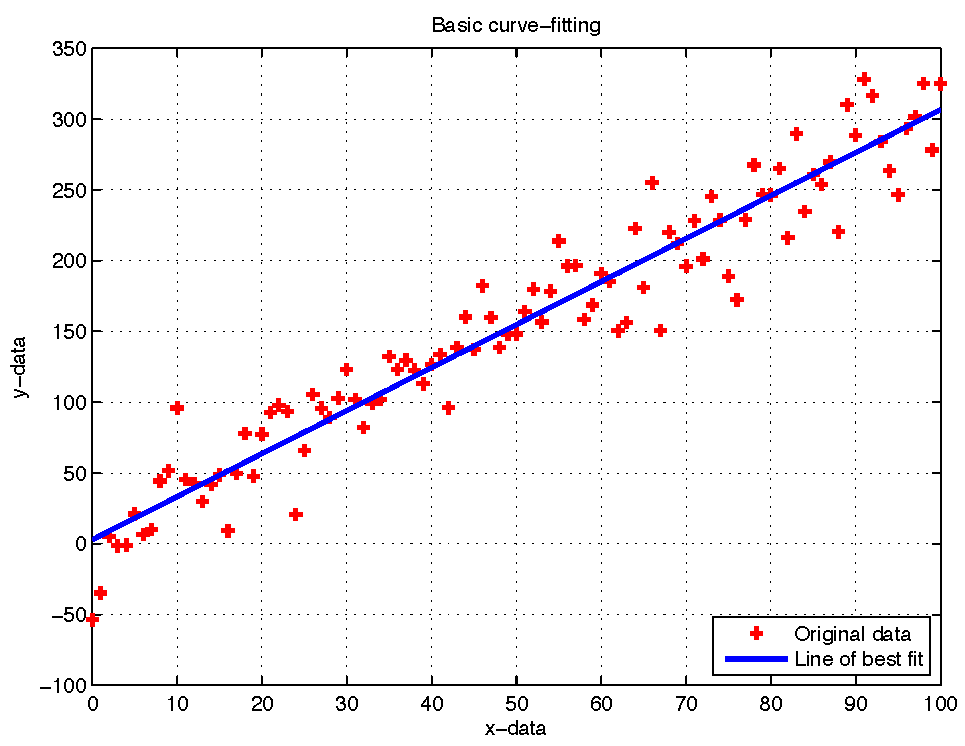
\includegraphics[width=\linewidth]{Graphics/Unit02/curve_fitting}
	\caption{Using \mcode{polyfit} and \mcode{polyval} for curve-fitting}
	\label{fig:curve_fitting}
\end{figure}

\section{\threed plotting using plot3 and surf}
\mlab is hugely powerful and versatile at visualising data in \threed. There are a number of built-in functions for producing different types of  \threed plots \eg\ points, lines, surfaces and volumes.

The \twod \mcode{plot} function becomes \mcode{plot3(x,y,z)} for plotting points and lines in \threed\ space. Listing~\ref{lst:3D-helix} and Figure~\ref{fig:3D-helix} demonstrate using \mcode{plot3} to plot the points on a helix in \threed space.
\begin{lstlisting}[caption={Using \mcode{plot3} to plot points on a helix},label=lst:3D-helix]
>> t = 0:pi/50:10*pi;
>> plot3(sin(t),cos(t),t,'r.'), grid on, ...
xlabel('x'), ylabel('y'), zlabel('z'), title('3D helix')
\end{lstlisting}
\begin{figure}
	\myfloatalign
	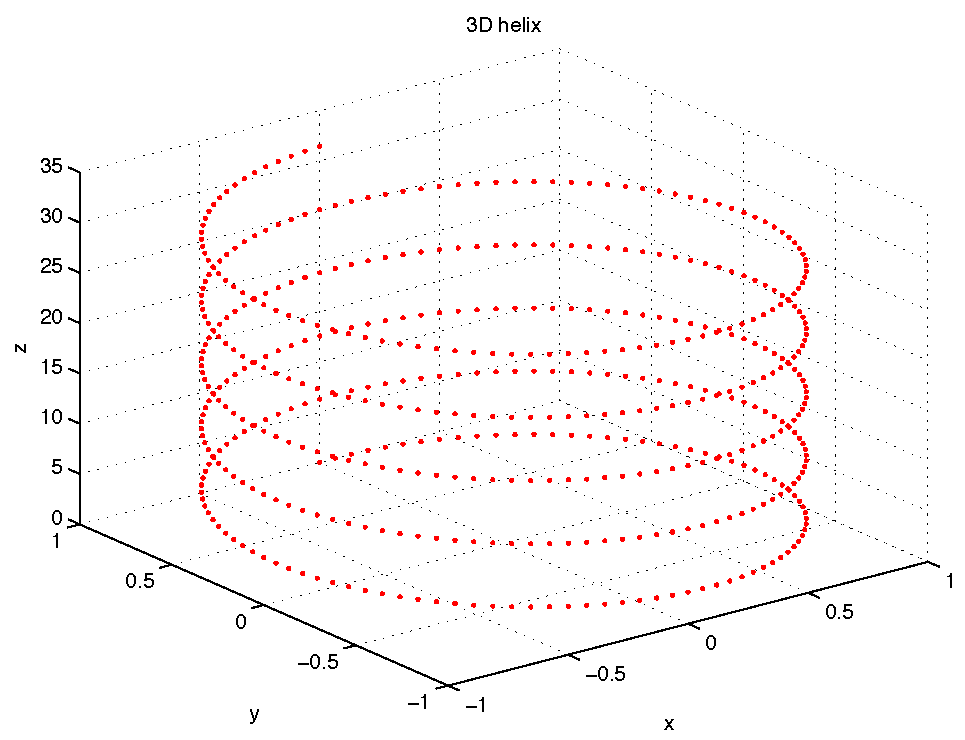
\includegraphics[width=\linewidth]{Graphics/Unit02/3D-helix}
	\caption{Using \mcode{plot3} to plot points on a helix}
	\label{fig:3D-helix}
\end{figure}

For plotting surfaces and contours two commonly used functions are \mcode{surf(x,y,z)} and \mcode{mesh(x,y,z)} where \mcode{x}, \mcode{y}, and \mcode{z} are coordinates of points on a surface. Before you use either of these functions you must use the \mcode{meshgrid} function to define a grid of points which the surface will be plotted onto. Listing~\ref{lst:meshgrid} demonstrates the typical use of \mcode{meshgrid}. In this example, assume $z=f(x,y)$ where $x$ is a vector of values $(1,2,3,4)$ and $y$ is a vector of values $(5,6,7)$. \mcode{meshgrid} takes the vectors $x$ and $y$ and returns two matrices, in this case called $xx$ and $yy$, which contain the coordinates of the grid that the surface $z$ will be plotted onto. Figure~\ref{fig:meshgrid} shows the coordinates of the points in the matrices returned by the \mcode{meshgrid} function.
\begin{figure}
	\myfloatalign
	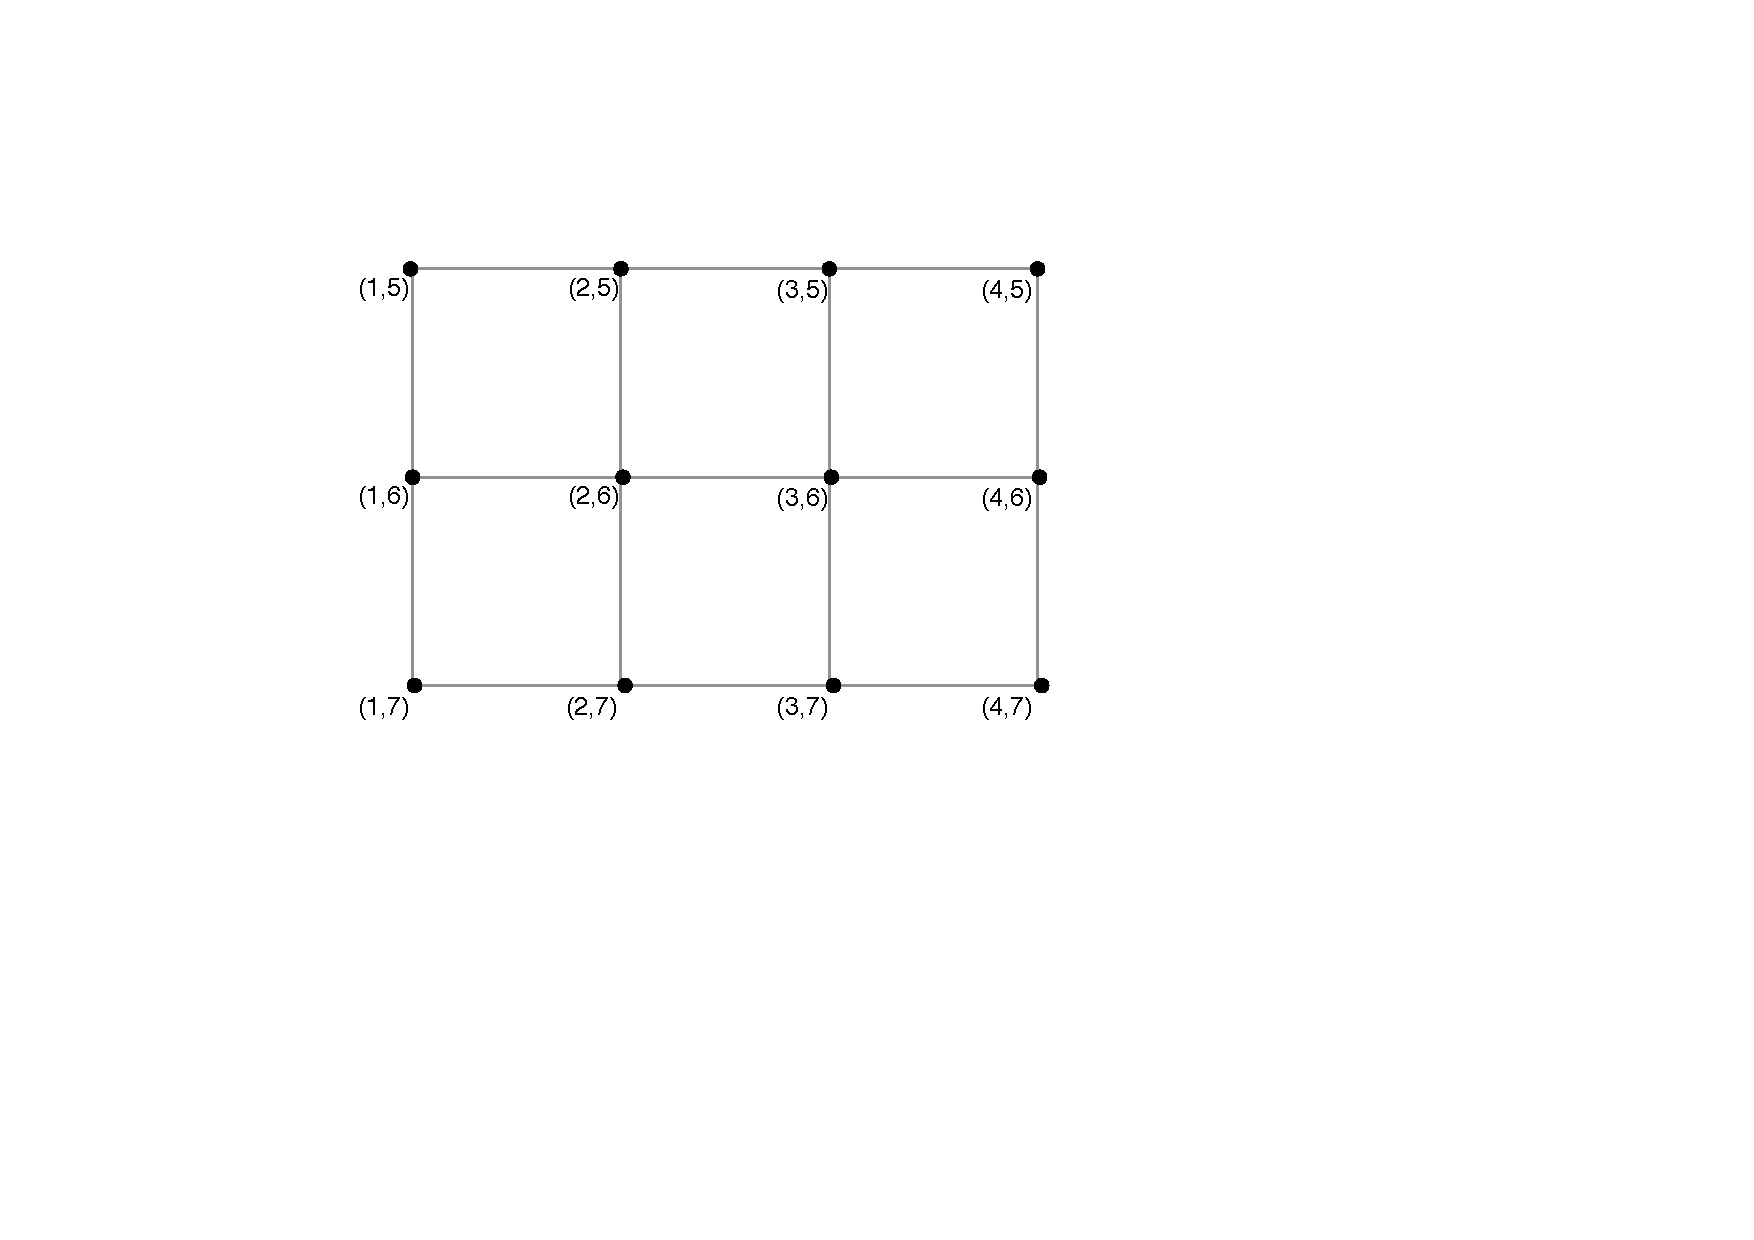
\includegraphics[width=0.70\linewidth]{Graphics/Unit02/meshgrid}
	\caption{Operation of \mcode{meshgrid} function}
	\label{fig:meshgrid}
\end{figure}

\begin{lstlisting}[caption={Using \mcode{meshgrid}},label=lst:meshgrid]
>> x = [1 2 3 4];
>> y = [5 6 7];
>> [xx, yy] = meshgrid(x,y)
xx =
     1     2     3     4
     1     2     3     4
     1     2     3     4
yy =
     5     5     5     5
     6     6     6     6
     7     7     7     7
\end{lstlisting}

\subsubsection{Comments:}
\begin{itemize}
\item \mcode{xx} is an array consisting of rows of the vector \mcode{x}.
\item \mcode{yy} is an array consisting of columns of vector \mcode{y}.
\item \mcode{xx} and \mcode{yy} are then used in the calculation of \mcode{z}, and the plotting of the surface. 
\end{itemize}
Listing~\ref{lst:surf} and Figures~\ref{fig:surf}--\ref{fig:mesh} demonstrate using \mcode{meshgrid} in combination with the surface plotting functions \mcode{surf} (creates a colour-filled surface) and \mcode{mesh} (creates a colored mesh) to plot the function:
\begin{equation*}
z=c \cdot \sin\left( 2\pi a \sqrt{x^2+y^2} \right),
\end{equation*}
where $a=3$, $c=0.5$, $-1\leq x \leq 1$, and $-1\leq y \leq 1$.
\begin{lstlisting}[caption={Plotting a surface},label=lst:surf]
>> x = linspace(-1,1,50);
>> y = x;
>> a = 3;
>> c = 0.5;
>> [xx, yy] = meshgrid(x,y);
>> z = c*sin(2*pi*a*sqrt(xx.^2+yy.^2));
>> surf(xx,yy,z), colorbar, xlabel('x'), ylabel('y'), zlabel('z'), ...
>> title('f(x,y)=csin(2\pia\surd(x^2+y^2))')
>> figure;
>> mesh(xx,yy,z), colorbar, xlabel('x'), ylabel('y'), zlabel('z'), ...
>> title('f(x,y)=csin(2\pia\surd(x^2+y^2))')
\end{lstlisting}
\begin{figure}[h!]
	\myfloatalign
	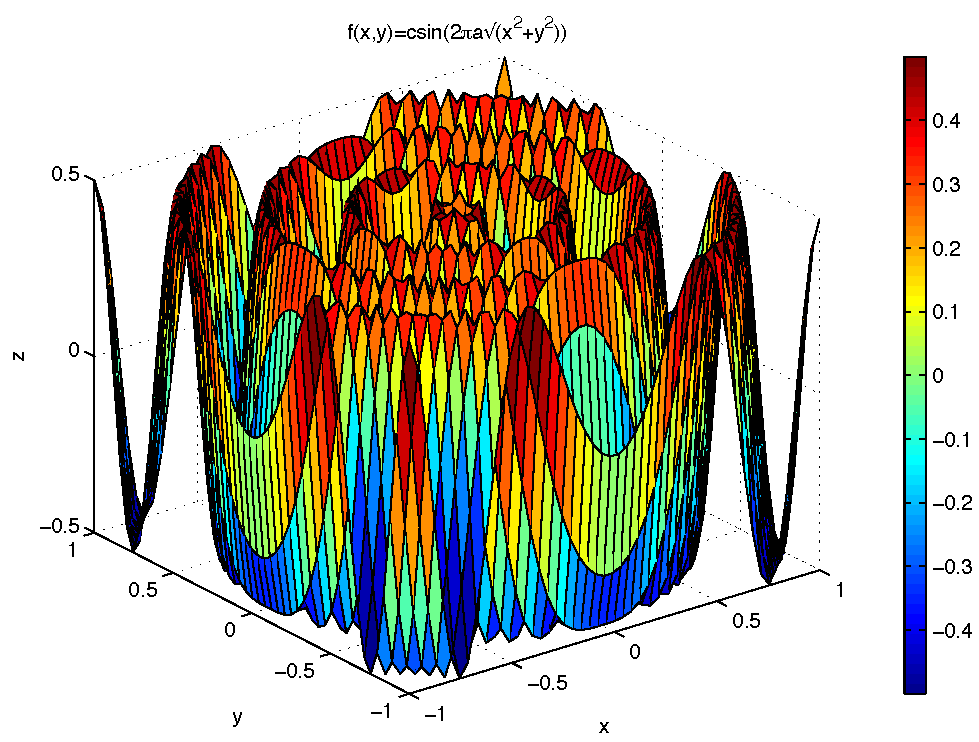
\includegraphics[width=\linewidth]{Graphics/Unit02/surf}
	\caption{Surface plot (using \mcode{surf}) of the function $z=c \cdot \sin( 2\pi a \sqrt{x^2+y^2})$}
	\label{fig:surf}
\end{figure}
\begin{figure}[h!]
	\myfloatalign
	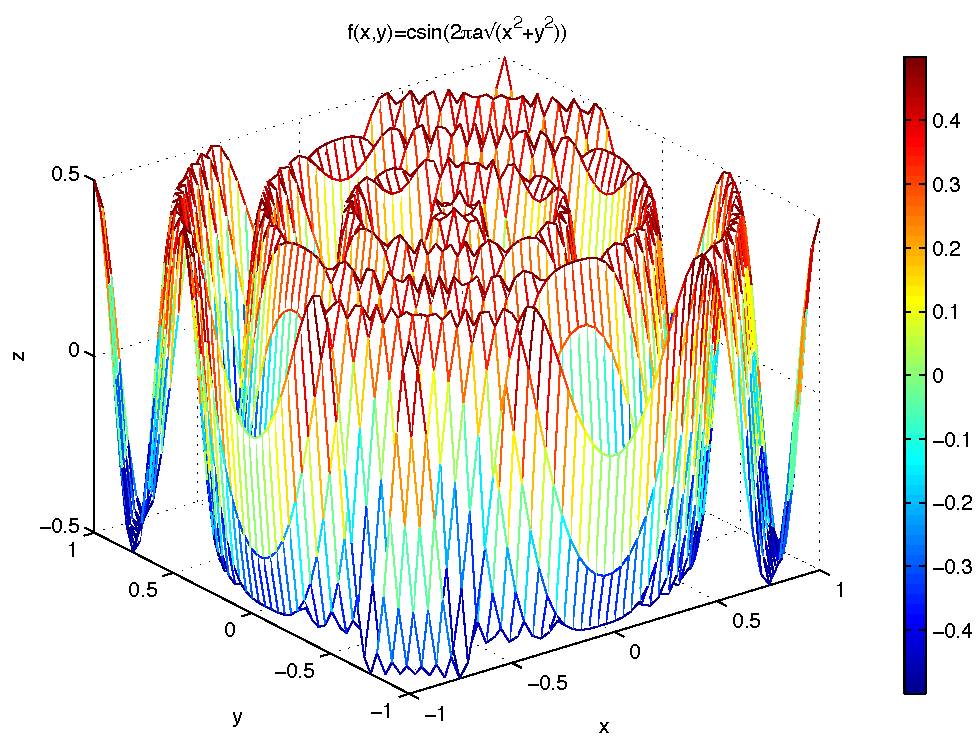
\includegraphics[width=\linewidth]{Graphics/Unit02/mesh}
	\caption{Surface plot (using \mcode{mesh}) of the function $z=c \cdot \sin( 2\pi a \sqrt{x^2+y^2})$}
	\label{fig:mesh}
\end{figure}

%%%%%%%%%%%%%%%%%%%%%%%%%%%%%%%%%%%%%%%%%%%%%%
% Exercise 4: 3D plotting
%%%%%%%%%%%%%%%%%%%%%%%%%%%%%%%%%%%%%%%%%%%%%%
\addtolength{\parindent}{-4mm}
\fcolorbox{myborderblue}{myblue}{%
\begin{minipage}{\linewidth}
\begin{minipage}{6mm}
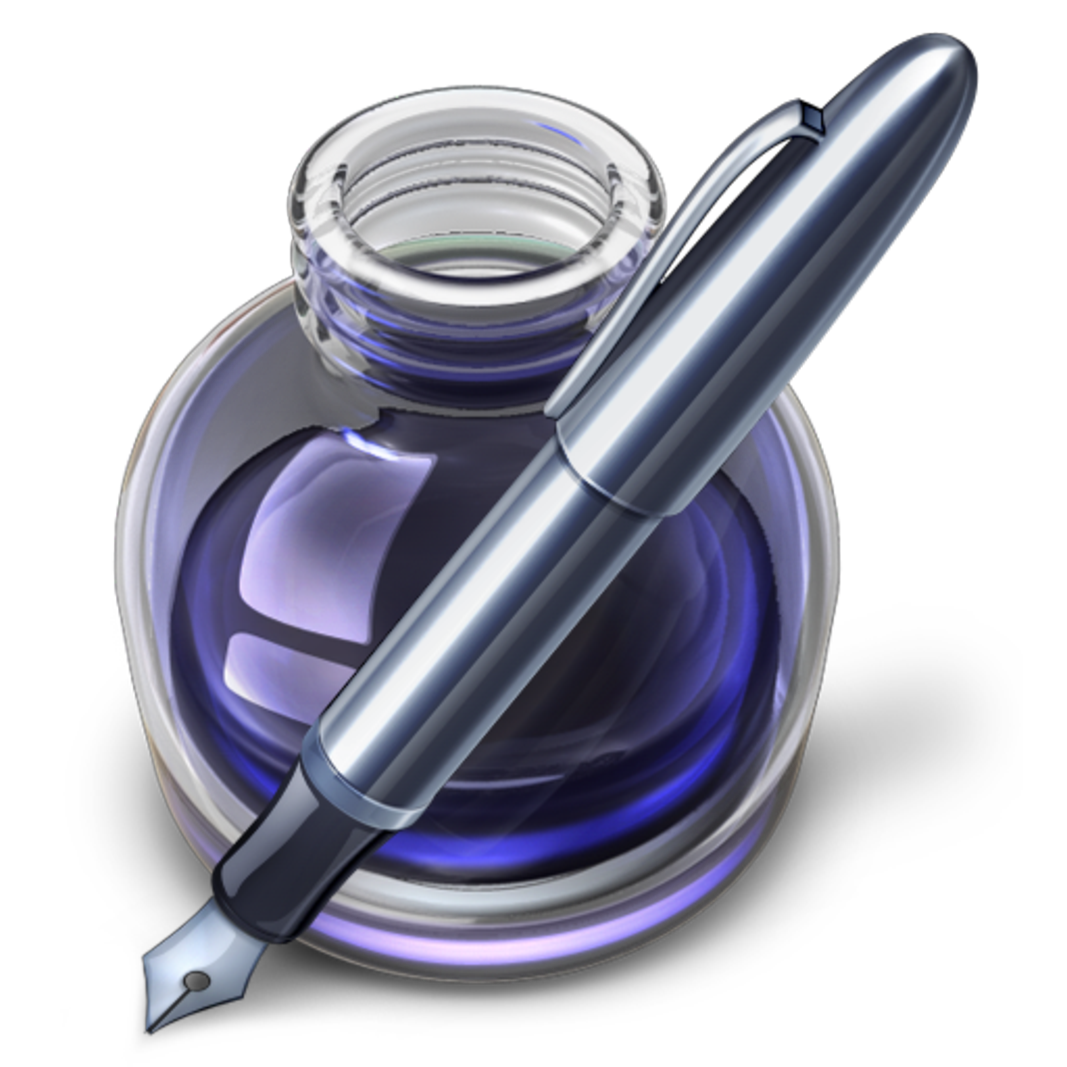
\includegraphics[scale=0.035]{Graphics/General/exercise_icon}
\end{minipage}
\exercise{\textit{Exercise 4: \threed plotting}}
\begin{enumerate}
\item Plot the following \threed curves using the \mcode{plot3} function:
	\begin{enumerate}
	\item \textit{Spherical helix}
		\begin{align*}
		x&= \sin\left(\frac{t}{2c}\right)\cos(t) \\
		y&= \sin\left(\frac{t}{2c}\right)\sin(t) \\
		z&= \cos\left(\frac{t}{2c}\right)
		\end{align*}
		where $c=5$ and $0 \leq t \leq 10\pi$.
	\item \textit{Sine wave on a sphere}
		\begin{align*}
		x&=\cos(t)\sqrt{b^2-c^2cos^2(at)} \\
		y&=\sin(t)\sqrt{b^2-c^2cos^2(at)} \\
		z&=c*\cos(at)
		\end{align*}
		where $a=10$, $b=1$, $c=0.3$, and $0 \leq t \leq 2\pi$.
	\end{enumerate}

\item Plot the following surfaces using the \mcode{surf} function:
	\begin{enumerate}
	\item \textit{Sine surface}
		\begin{align*}
		x&= \sin(u) \\
		y&= \sin(\nu) \\
		z&= \sin(u+\nu)
		\end{align*}
		where $0 \leq u \leq 2\pi$, and $0 \leq \nu \leq 2\pi$.
	\item \textit{Spring}
		\begin{align*}
		x&= \left[1-r_1 \cos(\nu)\right]\cos(u) \\
		y&= \left[1-r_1 \cos(\nu)\right]\sin(u) \\
		z&= r_2 \left[\sin(\nu)+\frac{tu}{\pi}\right]
		\end{align*}
		where $r_1=r_2=0.5$, $t=1.5$, $0 \leq u \leq 10\pi$, and $0 \leq \nu \leq 10\pi$.
	\item \textit{Elliptic torus}
		\begin{align*}
		x&= \left[c+\cos(\nu)\right]\cos(u) \\
		y&= \left[c+\cos(\nu)\right]\sin(u) \\
		z&= \sin(\nu)\cos(\nu)
		\end{align*}
		where $c=0.5$, $-\pi \leq u \leq \pi$, and $0 \leq \nu \leq \pi$. 
	\end{enumerate}
\end{enumerate}

\end{minipage}%
}\\
\addtolength{\parindent}{4mm}

%%%%%%%%%%%%%%%%%%%%%%%%%%%%%%%%%%%%%%%%%%%%%%
% Exercise 4: 3D plotting (continued)
%%%%%%%%%%%%%%%%%%%%%%%%%%%%%%%%%%%%%%%%%%%%%%
\addtolength{\parindent}{-4mm}
\fcolorbox{myborderblue}{myblue}{%
\begin{minipage}{\linewidth}
\begin{minipage}{6mm}
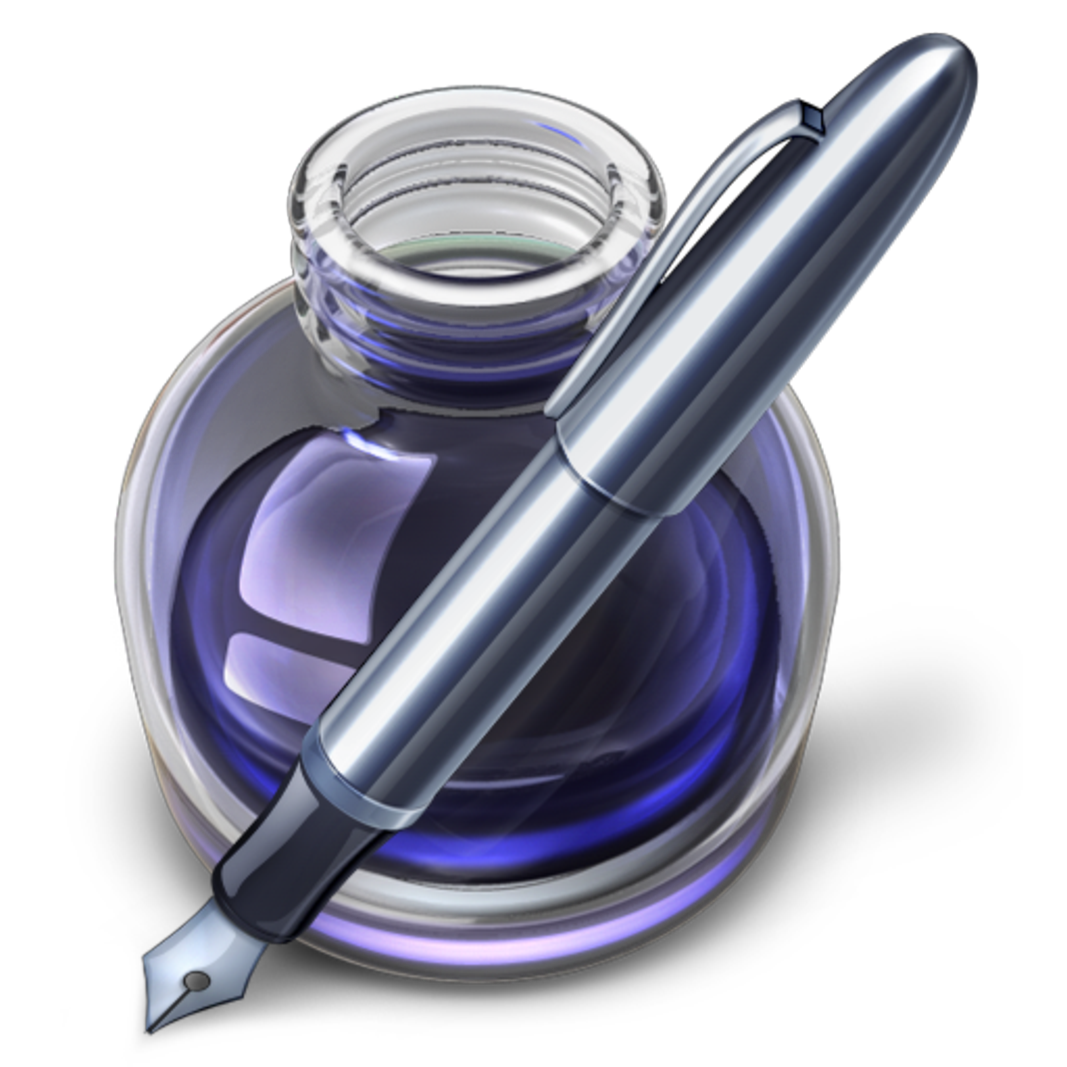
\includegraphics[scale=0.035]{Graphics/General/exercise_icon}
\end{minipage}
\textit{Exercise 4: \threed plotting (continued)}
\begin{itemize}
	\item Use the \mcode{shading interp} command after \mcode{surf} to change the shading type.
	\item Add a \mcode{colorbar} to the plots.
\end{itemize}	

%%%%%%%%%%%%%%%%%%%%%%%%%%%%%%%%%%%%%%%%%%%%%%
% Screencast: Exercise 4 Solutions
%%%%%%%%%%%%%%%%%%%%%%%%%%%%%%%%%%%%%%%%%%%%%%
\begin{minipage}{6mm}

\includegraphics[scale=0.03]{Graphics/General/screencast_icon}
\end{minipage}
\href{http://www.eng.ed.ac.uk/teaching/courses/matlab/unit02/Ex4-Solutions.shtml}{\screencast{Exercise 4 Solutions}}\\
(http://www.eng.ed.ac.uk/teaching/courses/matlab/unit02/Ex4-Solutions.shtml)
\end{minipage}%
}\\
\addtolength{\parindent}{4mm}

\vspace{5mm}
%%%%%%%%%%%%%%%%%%%%%%%%%%%%%%%%%%%%%%%%%%%%%%
% Reference to additional exercises
%%%%%%%%%%%%%%%%%%%%%%%%%%%%%%%%%%%%%%%%%%%%%%
\addtolength{\parindent}{-4mm}
\fcolorbox{myborderblue}{myblue}{%
\begin{minipage}{\linewidth}
\begin{minipage}{6mm}
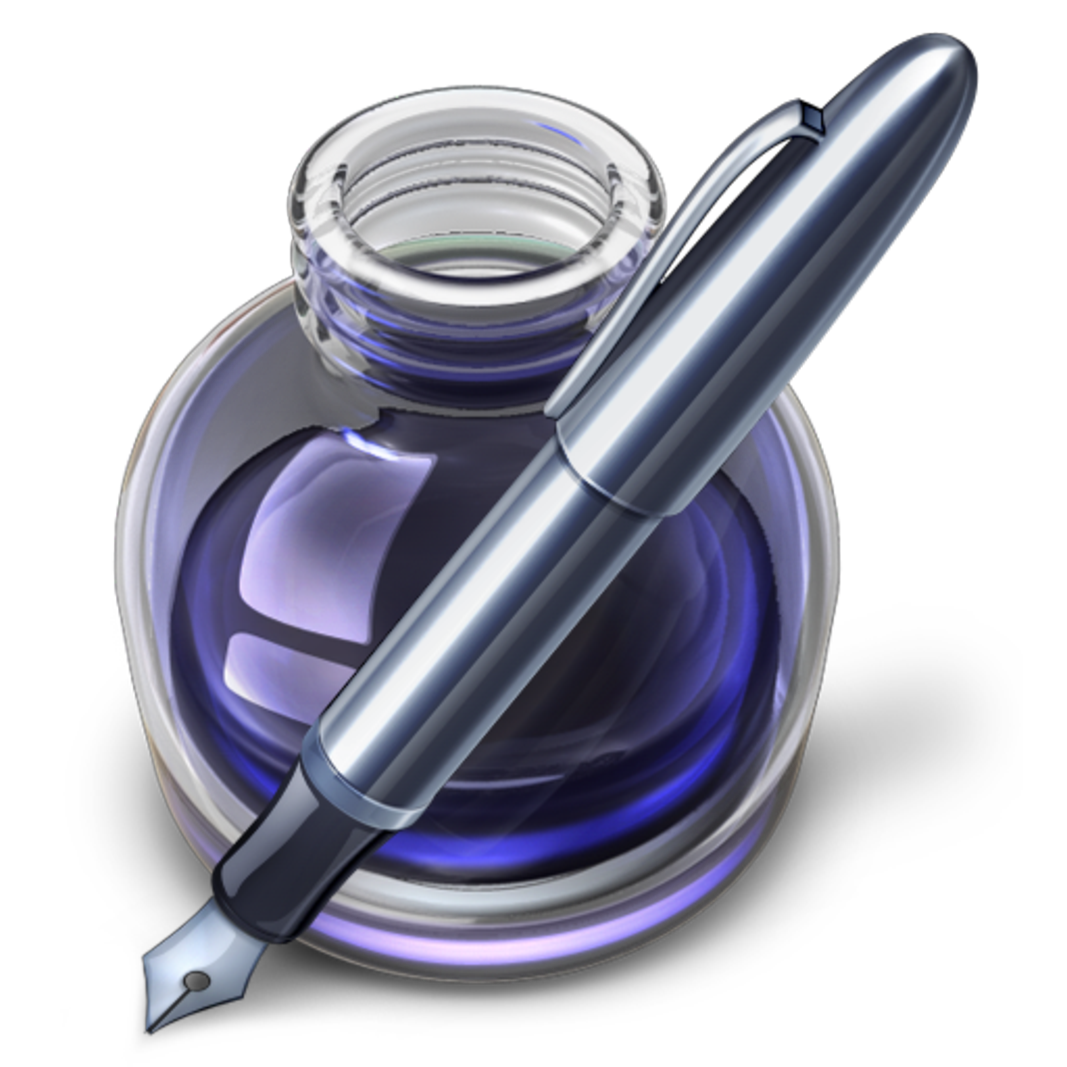
\includegraphics[scale=0.035]{Graphics/General/exercise_icon}
\end{minipage}
\textit{Additional Exercises}\\
You should now attempt questions from Chapter~\ref{sect:plotting}. 
\end{minipage}%
}\\
\addtolength{\parindent}{4mm}
\chapter{Scripts and Functions}

\section{Script files}
A \textit{script} file is a text file that contains a series of \mlab commands that you would type at the command prompt. A \textit{script} file is one type of m-file (\textit{.m} file extension), the other type being a \textit{function} file which will be examined in Section~\ref{sec:functions}. Script files are useful when you have to repeat a set of commands, often only changing the value of one variable every time. By writing a script file you are saving your work for later use. Script files work on variables in the current workspace, and results obtained from running a script are left in the current workspace.

New script files can be created by clicking on the \textit{New M-File} icon in the \mlab Window toolbar, shown in Figure~\ref{fig:new_script}. This launches the \mlab Editor with a blank M-File.
\begin{figure}[h]
	\myfloatalign
	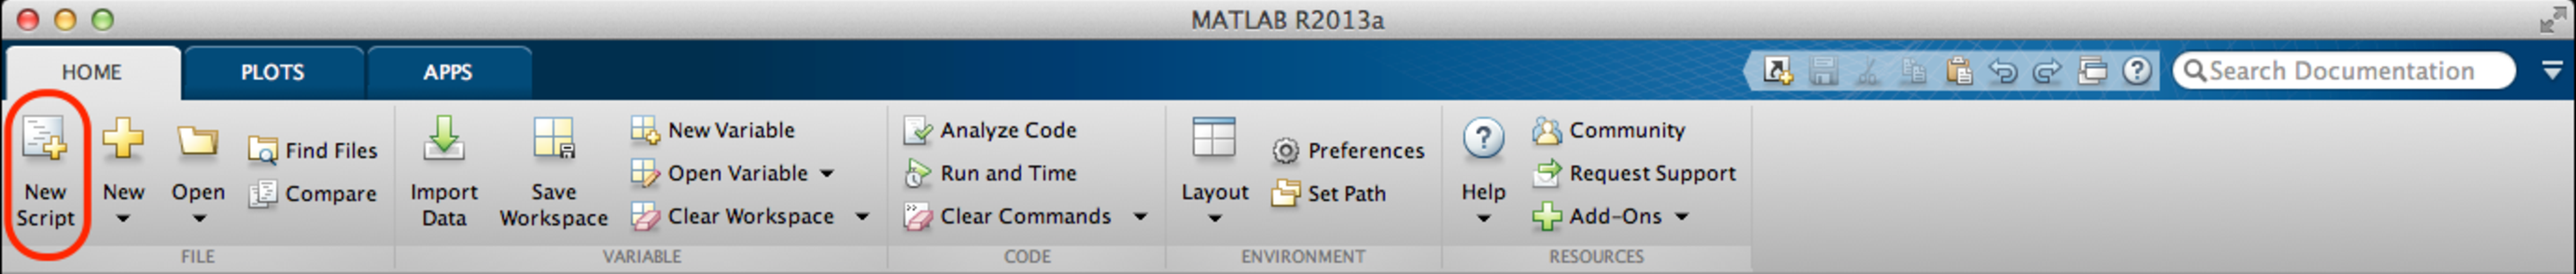
\includegraphics[width=0.9\linewidth]{Graphics/Unit03/new_script}
	\caption{\textit{New M-File} toolbar icon in \mlab Window}
	\label{fig:new_script}
\end{figure}

Listing~\ref{lst:my_surf} presents the commands from Listing~\ref{lst:surf} in the form of a script file. The script file has been saved as \textit{my\_surf.m}, and can be run by either typing \mcode{my_surf} at the command prompt, or clicking the \textit{Save and run} icon in the Editor Window toolbar, as shown in Figure~\ref{fig:run_script}. Copy and paste the example into a new script file, and run it to see the results for yourself.
\begin{figure}[h]
	\myfloatalign
	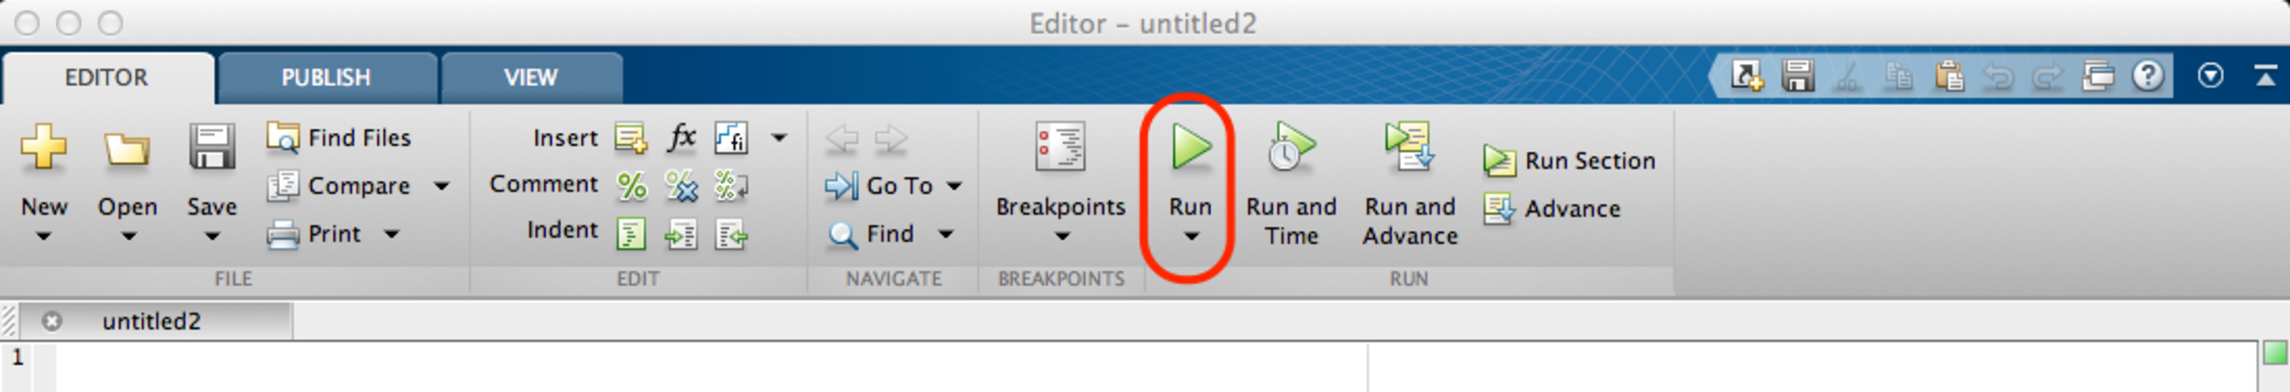
\includegraphics[width=0.9\linewidth]{Graphics/Unit03/run_script}
	\caption{\textit{Save and run} toolbar icon in Editor Window}
	\label{fig:run_script}
\end{figure}

\newpage
\lstinputlisting[caption={\textit{my\_surf.m} - Script to plot a surface},label=lst:my_surf]{MATLAB-code/Document/my_surf.m}

\subsubsection{Comments:}
\begin{itemize}
\item It is extremely useful, for both yourself and others, to put comments in your script files. A comment is always preceded with a percent sign (\mcode{\%}) which tells \mlab not to execute the rest of the line as a command.
\item Script file names MUST NOT contain spaces (replace a space with the underscore), start with a number, be names of built-in functions, or be variable names.
\item It is a good idea to use the \mcode{clear all} and \mcode{clc} commands as the first commands in your script to clear any existing variables from the \mlab workspace and clear up the Command Window before you begin.
\end{itemize}

\addtolength{\parindent}{-4mm}
\fcolorbox{myborderblue}{myblue}{%
\begin{minipage}{\linewidth}
\begin{minipage}{6mm}

\includegraphics[scale=0.03]{Graphics/General/help_icon}
\end{minipage}
\textit{Writing good scripts} \\
Here are some useful tips that you should follow to make your script files easy to follow and easy to understand by others, or even yourself after a few weeks!\footnote{Adapted from \citet{Patzer:2003fk}.}
\begin{itemize}
\item Script files should have a header section that identifies:
	\begin{itemize}
	\item What the program does
	\item Who the author is
	\item When the program was written or last revised
	\item The variable dictionary \ie\ a list of all variables their meanings and units
	\end{itemize}
\item Use plenty of white space to make your program easy to read.
\item Use plenty of comments! In particular define all variables and their units in the variable dictionary.
\item Use meaningful names for variables. Don't be afraid of being verbose \eg\ use \mcode{steel_area} in preference to \mcode{sa}.
\item Remember to use the \mcode{clear all} and \mcode{clc} commands at the start of your script.
\end{itemize}
\end{minipage}%
}\\
\addtolength{\parindent}{4mm}
\vspace{5mm}

%%%%%%%%%%%%%%%%%%%%%%%%%%%%%%%%%%%%%%%%%%%%%%
% Screencast: Creating a simple script
%%%%%%%%%%%%%%%%%%%%%%%%%%%%%%%%%%%%%%%%%%%%%%
\addtolength{\parindent}{-4mm}
\fcolorbox{myborderblue}{myblue}{%
\begin{minipage}{\linewidth}
\begin{minipage}{6mm}

\includegraphics[scale=0.03]{Graphics/General/screencast_icon}
\end{minipage}
\href{http://www.eng.ed.ac.uk/teaching/courses/matlab/unit03/simple-script.shtml}{\screencast{Creating a simple script}}\\
(http://www.eng.ed.ac.uk/teaching/courses/matlab/unit03/simple-script.shtml)
\end{minipage}%
}\\
\addtolength{\parindent}{4mm}
\vspace{5mm}

\addtolength{\parindent}{-4mm}
\fcolorbox{myborderblue}{myblue}{%
\begin{minipage}{\linewidth}
\begin{minipage}{6mm}
\includegraphics[scale=0.03]{Graphics/General/help_icon}
\end{minipage}
\textit{The \mcode{input} function} \\
The \mcode{input} function is used to request user input and assign it to a variable. For example \mcode{x = input('Enter a number: ');} will display the text \mcode{Enter a number: } in the Command Window and then wait until the user enters something. Whatever is entered will be assigned to the variable \mcode{x}.
\end{minipage}%
}\\
\addtolength{\parindent}{4mm}
\vspace{5mm}

\addtolength{\parindent}{-4mm}
\fcolorbox{myborderblue}{myblue}{%
\begin{minipage}{\linewidth}
\begin{minipage}{6mm}
\includegraphics[scale=0.03]{Graphics/General/help_icon}
\end{minipage}
\textit{The \mcode{disp} function} \\
The \mcode{disp} function can be used display strings of text to the Command Window \eg\ \mcode{disp('I am a string of text')}. You can also display numbers by converting them to strings \eg\ \mcode{disp(num2str(10))}. The \mcode{num2str} function simply converts the number 10 to a string that can be displayed by the \mcode{disp} function. You can also combine the display of text and numbers \eg\ \mcode{disp(['Factorial '} \mcode{num2str(x) ' is '} \mcode{num2str(y)])}. Notice the use of spaces to denote the separate elements of the string, and square brackets around the string to concatenate it together.
\end{minipage}%
}\\
\addtolength{\parindent}{4mm}

%%%%%%%%%%%%%%%%%%%%%%%%%%%%%%%%%%%%%%%%%%%%%%
% Exercise 5: Scripts
%%%%%%%%%%%%%%%%%%%%%%%%%%%%%%%%%%%%%%%%%%%%%%
\addtolength{\parindent}{-4mm}
\fcolorbox{myborderblue}{myblue}{%
\begin{minipage}{\linewidth}
\begin{minipage}{6mm}
\includegraphics[scale=0.035]{Graphics/General/exercise_icon}
\end{minipage}
\exercise{\textit{Exercise 5: Scripts}} \\
Write your own script files to solve the following problems:
\begin{enumerate}
\item The absolute pressure at the bottom of a liquid store tank that is vented to the atmosphere is given by:
\begin{equation*}
P_{\textrm{abs,bottom}} = \rho g h + P_{\textrm{outside}},
\end{equation*}
where:
\begin{align*}
P_{\textrm{abs,bottom}} &= \textrm{the absolute pressure at the bottom of the storage tank ($Pa$)} \\
\rho &= \textrm{liquid density ($kg/m^3$)} \\
g &= \textrm{acceleration due to gravity ($m/s^2$)} \\
h &= \textrm{height of the liquid ($m$)} \\
P_{\textrm{outside}} &= \textrm{outside atmospheric pressure ($Pa$)}
\end{align*}
Find $P_{\textrm{abs,bottom}}$ in SI units if $\rho=1000~kg/m^3$, $g=32.2~ft/s^2$, $h=7~yd$, and $P_{\textrm{outside}}=1~atm$. \\
Here are some tips to help you get started:
	\begin{itemize}
	\item Remember your header section and variable dictionary.
	\item Use \mcode{input} functions to gather information from the user.
	\item Convert all units to SI before performing the calculation. Use the following conversion factors:
		\renewcommand{\labelitemii}{}
		\begin{itemize}
		\item \mcode{ft_to_m = 0.3048}
		\item \mcode{yd_to_m = 0.9144}
		\item \mcode{atm_to_Pa = 1.013E5}
		\end{itemize}
	\item Calculate $P_{\textrm{abs,bottom}}$
	\end{itemize}
\footnotesize{\textit{[Answers: $164121~Pa$]}\\
Example adapted from \citet{Patzer:2003fk}}	
\normalsize
\end{enumerate}
\end{minipage}%
}\\
\addtolength{\parindent}{4mm}

%%%%%%%%%%%%%%%%%%%%%%%%%%%%%%%%%%%%%%%%%%%%%%
% Exercise 5: Scripts (continued)
%%%%%%%%%%%%%%%%%%%%%%%%%%%%%%%%%%%%%%%%%%%%%%
\addtolength{\parindent}{-4mm}
\fcolorbox{myborderblue}{myblue}{%
\begin{minipage}{\linewidth}
\begin{minipage}{6mm}
\includegraphics[scale=0.035]{Graphics/General/exercise_icon}
\end{minipage}
\textit{Exercise 5: Scripts (continued)}
\begin{enumerate}
\setcounter{enumi}{1}
\item A pipeline at an oil refinery is carrying oil to a large storage tank. The pipe has a 20~inch internal diameter. The oil is flowing at 5~$ft/s$ and its density is 57~$lb/ft^3$. What is the mass flow rate of oil in SI units? What is the mass and volume of oil, in SI units, that flows in a 24~hour period? The flow rate of oil is given by:
\begin{equation*}
\dot{M} = \rho \nu A,
\end{equation*}
where:
\begin{align*}
\dot{M} &= \textrm{mass flow rate of oil ($kg/s$)} \\
\rho &= \textrm{liquid density ($kg/m^3$)} \\
\nu &= \textrm{flow speed ($m/s$)} \\
A &= \textrm{cross-sectional area of pipe ($m^2$)}
\end{align*}
\footnotesize{\textit{[Answers: $282~kg/s$, $24362580~kg$, $26688~m^3$]}\\
Example adapted from \citet{Moore:2009fk}}
\normalsize

\item The current in a resistor/inductor circuit is given by:
\begin{align*}
I(t) &= \frac{\nu_0}{|Z|} \left[ \cos(\omega t - \phi) - e^{-\frac{tR}{L}} \cos(\phi) \right],
\end{align*}
where:
\begin{align*}
\omega & = 2\pi f, \\
Z &= (R + j \omega L), \\
\phi &= \tan^{-1}\left(\frac{\omega L}{R}\right),
\end{align*}
and where:
\begin{align*}
\nu_0 &= \textrm{voltage ($V$)} \\
\omega &= \textrm{angular frequency ($rads/s$)} \\
R &= \textrm{resistance ($\Omega$)} \\
L &= \textrm{inductance ($H$)}
\end{align*}
Find and plot $I(t)$ if $\nu_0=230~V$, $f=50~Hz$, $R=500~\Omega$, and $L=650~mH$.
\begin{itemize}
	\item You'll need to explore different values of $t$ to find one that best plots the behaviour of the current.
	\end{itemize}
\end{enumerate}

%%%%%%%%%%%%%%%%%%%%%%%%%%%%%%%%%%%%%%%%%%%%%%
% Screencast: Exercise 5 Solutions
%%%%%%%%%%%%%%%%%%%%%%%%%%%%%%%%%%%%%%%%%%%%%%
\begin{minipage}{6mm}
\includegraphics[scale=0.03]{Graphics/General/screencast_icon}
\end{minipage}
\href{http://www.eng.ed.ac.uk/teaching/courses/matlab/unit03/Ex5-Solutions.shtml}{\screencast{Exercise 5 Solutions}}\\
(http://www.eng.ed.ac.uk/teaching/courses/matlab/unit03/Ex5-Solutions.shtml)
\end{minipage}%
}\\
\addtolength{\parindent}{4mm}
\vspace{5mm}

\addtolength{\parindent}{-4mm}
\fcolorbox{myborderblue}{myblue}{%
\begin{minipage}{\linewidth}
\begin{minipage}{6mm}
\includegraphics[scale=0.03]{Graphics/General/help_icon}
\end{minipage}
\textit{The \mcode{abs} function} \\
The \mcode{abs} function can be used to calculate the absolute value or magnitude of a number.
\end{minipage}%
}\\
\addtolength{\parindent}{4mm}

\section{Functions}\label{sec:functions}
Another type of m-file (\textit{.m} file extension) is a function file. Functions are similar to scripts, except that the variables in a function are only available to the function itself \ie\ are local to the function. This is in contrast with script files, where any variables you define exist in the  Workspace (are global) and can be used by other scripts and commands. You have used many of the built-in functions in \mlab \eg\ \mcode{size}, \mcode{plot}, \mcode{surf} \etc, and as you become more familiar with \mlab you will learn to write your own functions to perform specific tasks. 

A function file always begins with a function definition line. This specifies the input and output variables that the function will use, and defines a name for the function. Listing~\ref{lst:function_syntax} presents the syntax of a function definition line, and Table~\ref{tab:function_defs} gives some examples.
\begin{lstlisting}[caption={Syntax of a function definition},label=lst:function_syntax]
function [outputVariables] = functionName (inputVariables)
% Comments describing function and variables
commands
\end{lstlisting}
\begin{sidewaystable}
	\caption{Function definitions, filenames, input and output variables}
	\label{tab:function_defs}
	\myfloatalign
	\begin{tabular}{lcccl}\toprule
	\spacedlowsmallcaps{Function definition} & \spacedlowsmallcaps{Filename} & \spacedlowsmallcaps{Input variables} & \spacedlowsmallcaps{Output variables} & \spacedlowsmallcaps{Notes} \\ \midrule
	\mcode{function [rho, H, F] = motion(x, y, t)} & \textit{motion.m} & \mcode{x, y, t} & \mcode{rho, H, F} & \\
	\mcode{function [theta] = angleTH(x, y)} & \textit{angleTH.m} & \mcode{x, y} & \mcode{theta} & \\
	\multirow{4}{*}{\mcode{function theta = THETA(x, y)}} & \multirow{4}{*}{\textit{THETA.m}} & \multirow{4}{*}{\mcode{x, y}} & \multirow{4}{*}{\mcode{theta}} & If there is only one \\ 
	& & & & output variable the \\
	& & & & square brackets can \\
	& & & & be omitted\\
	\mcode{function [] = circle(r)} & \textit{circle.m} & \mcode{r} & None & \\
	\multirow{5}{*}{\mcode{function circle(r)}} & \multirow{5}{*}{\textit{circle.m}} & \multirow{5}{*}{\mcode{r}} & \multirow{5}{*}{None} & If there are no \\ 
	& & & & output variables the \\
	& & & & square brackets and \\
	& & & & the equals sign \\
	& & & & can be omitted\\
	\bottomrule
	\end{tabular}
\end{sidewaystable}

\subsubsection{Comments:}
\begin{itemize}
\item The first word, \mcode{function}, is mandatory, and tells \mlab this m-file in a function file.
\item On the lefthand side of the equals sign is a list of the output variables that the function will return. You will notice when there is more than one output variable, that they are enclosed in \textit{square} brackets.
\item On the righthand side of the equals sign is the name of the function. You must save your function file with the same name that you use here.\graffito{The name used to save a function file must match the function name.}
\item Lastly, within the \textit{round} brackets after the function name, is a comma separated list of the input variables.
\item It is good practice to put some comments after the function definition line to explain what task the function performs and how you should use the input and output variables. This is in addition to comments you would usually include at the top of a script file.
\end{itemize}

Functions are executed at the command prompt by typing their function definition line without the \mcode{function} command. Listing~\ref{lst:function_exe} demonstrates how you would execute the \mcode{motion} function from Table~\ref{tab:function_defs}.
\begin{lstlisting}[caption={Executing a function},label=lst:function_exe]
>> [rho, H, F] = motion(x, y, t)
\end{lstlisting}

\subsubsection{Comments:}
\begin{itemize}
\item Input variables \mcode{x, y, t} must be defined in the workspace before you execute the function. This is because variables defined within a function file are local to the function, i.e. do not exist in the workspace.
\item When you execute the function the names for the input and output variables do not have to match those used in the function file.
\end{itemize}
\newpage
Listings~\ref{lst:simple_function} presents an example of a simple function that multiplies two numbers, \mcode{x} and \mcode{y}, together to calculate an \mcode{area}. Listing~\ref{lst:simple_function_exe1} demonstrates how to execute this function in the command window.

\begin{lstlisting}[caption={A simple function},label=lst:simple_function]
function area = calculateArea(x, y)
% Function to calculate an area given two lengths (x, y)
area = x*y;
\end{lstlisting}

\begin{lstlisting}[caption={Execution of a simple function},label=lst:simple_function_exe1]
>> x = 5; y = 10;
>> area = calculateArea(x, y)
area = 
    50
\end{lstlisting}

The same function could also be executed using variables with different names, as shown in Listing~\ref{lst:simple_function_exe2}.
\begin{lstlisting}[caption={Execution of a simple function},label=lst:simple_function_exe2]
>> length1 = 25; length2 = 100;
>> myArea = calculateArea(length1, length2)
myArea = 
      2500
\end{lstlisting}
\vspace{5mm}

%%%%%%%%%%%%%%%%%%%%%%%%%%%%%%%%%%%%%%%%%%%%%%
% Screencast: Creating a function
%%%%%%%%%%%%%%%%%%%%%%%%%%%%%%%%%%%%%%%%%%%%%%
\addtolength{\parindent}{-4mm}
\fcolorbox{myborderblue}{myblue}{%
\begin{minipage}{\linewidth}
\begin{minipage}{6mm}
\includegraphics[scale=0.03]{Graphics/General/screencast_icon}
\end{minipage}
\href{http://www.eng.ed.ac.uk/teaching/courses/matlab/unit03/simple-function.shtml}{\screencast{Creating a function}}\\
(http://www.eng.ed.ac.uk/teaching/courses/matlab/unit03/simple-function.shtml)
\end{minipage}%
}\\
\addtolength{\parindent}{4mm}

%%%%%%%%%%%%%%%%%%%%%%%%%%%%%%%%%%%%%%%%%%%%%%
% Exercise 6: Functions
%%%%%%%%%%%%%%%%%%%%%%%%%%%%%%%%%%%%%%%%%%%%%%
\addtolength{\parindent}{-4mm}
\fcolorbox{myborderblue}{myblue}{%
\begin{minipage}{\linewidth}
\begin{minipage}{6mm}
\includegraphics[scale=0.035]{Graphics/General/exercise_icon}
\end{minipage}
\exercise{\textit{Exercise 6: Functions}} \\
Write your own functions to solve the following problems:
\begin{enumerate}
\item Produce a conversion table for Celsius and Fahrenheit temperatures. The input to the function should be two numbers: $T_{\textrm{lower}}$ and $T_{\textrm{upper}}$ which define the lower and upper range, in Celsius, for the table. The output of the function should be a two column matrix with the first column showing the temperature in Celsius, from $T_{\textrm{lower}}$ and $T_{\textrm{upper}}$ with an increment of 1~$^\circ$C, and the second column showing the corresponding temperature in Fahrenheit. \\
Here are some tips to help you get started:
	\begin{itemize}
	\item Start with a function definition line. What are your input and output variables?
	\item Create a column vector to hold the range \mcode{Celsius = [T_lower:T_upper]'}
	\item Calculate the corresponding values in Fahrenheit using \mcode{Fahrenheit = 9/5 * Celsius + 32}
	\item Create a matrix to hold the table using \mcode{temp_table = [Celsius Fahrenheit]}
	\end{itemize}
Test your function for $T_{\textrm{lower}}=0~^{\circ}C$ and $T_{\textrm{upper}}=25~^{\circ}C$.
\item The angles of cosines of a vector in \threed space are given by:
\begin{equation*}
\cos(\alpha_j) = \frac{a_j}{|a|}, \quad \textrm{for} \quad j=1,2,3 
\end{equation*}
Given the magnitude, $|a|$, and angles of cosines, $\alpha_j$, calculate the Cartesian components, $a_j$, of the vector.
\end{enumerate}

%%%%%%%%%%%%%%%%%%%%%%%%%%%%%%%%%%%%%%%%%%%%%%
% Screencast: Exercise 6 Solutions
%%%%%%%%%%%%%%%%%%%%%%%%%%%%%%%%%%%%%%%%%%%%%%
\begin{minipage}{6mm}
\includegraphics[scale=0.03]{Graphics/General/screencast_icon}
\end{minipage}
\href{http://www.eng.ed.ac.uk/teaching/courses/matlab/unit03/Ex6-Solutions.shtml}{\screencast{Exercise 6 Solutions}}\\
(http://www.eng.ed.ac.uk/teaching/courses/matlab/unit03/Ex6-Solutions.shtml)
\end{minipage}%
}\\
\addtolength{\parindent}{4mm}

\vspace{5mm}
%%%%%%%%%%%%%%%%%%%%%%%%%%%%%%%%%%%%%%%%%%%%%%
% Reference to additional exercises
%%%%%%%%%%%%%%%%%%%%%%%%%%%%%%%%%%%%%%%%%%%%%%
\addtolength{\parindent}{-4mm}
\fcolorbox{myborderblue}{myblue}{%
\begin{minipage}{\linewidth}
\begin{minipage}{6mm}
\includegraphics[scale=0.035]{Graphics/General/exercise_icon}
\end{minipage}
\textit{Additional Exercises}\\
You should now attempt questions from Chapter~\ref{sect:scripts_functions}. 
\end{minipage}%
}\\
\addtolength{\parindent}{4mm}
\chapter{Decision making}
All the problems you have solved so far have been problems with a \textit{straight-line} logic pattern \ie\ you followed a sequence of steps (defining variables, performing calculations, displaying results) that flowed directly from one step to another. Decision making is an important concept in programming and allows you to control which parts of your code should execute depending on certain conditions. This flow of control in your program can be performed by branching with \mcode{if} and \mcode{else} statements, which will be discussed in this chapter, or looping, which will be discussed in Chapter~\ref{ch:loops}. 

\section{Relational and logical operations}
Relational and logical operators are used in branching and looping to help make decisions. The result of using a relational or logical operator will always be either true, given by a \mcode{1}, or false, given by a \mcode{0}. Tables~\ref{tab:relational_ops}--\ref{tab:logical_ops} list the most common relational and logical operators in \mlab.

\begin{table}[h]
	\caption{Relational operators}
	\label{tab:relational_ops}
	\myfloatalign
	\begin{tabular}{lcc}\toprule
	\spacedlowsmallcaps{Operator} & \spacedlowsmallcaps{Mathematical symbol} & \spacedlowsmallcaps{\mlab symbol} \\ \midrule
	Equal & $=$ & $==$ \\
	Not equal & $\neq$ & $\sim=$ \\
	Less than & $<$ & $<$ \\
	Greater than & $>$ & $>$ \\
	Less than or equal & $\leq$ & $<=$ \\
	Greater than or equal & $\geq$ & $>=$\\
	\bottomrule
	\end{tabular}
\end{table}

\begin{table}[h]
	\caption{Logical operators}
	\label{tab:logical_ops}
	\myfloatalign
	\begin{tabular}{lcc}\toprule
	\spacedlowsmallcaps{Operator} & \spacedlowsmallcaps{Mathematical symbol} & \spacedlowsmallcaps{\mlab symbol} \\ \midrule
	And & AND & $\&$ \\
	Or & OR & $|$ \\
	Not & NOT & $\sim$ \\
	\bottomrule
	\end{tabular}
\end{table}
\newpage
Listings~\ref{lst:simple_relational_ops} presents a simple example of using relational operators.
\begin{lstlisting}[caption={Simple relational operators},label=lst:simple_relational_ops]
>> x = 5;
>> y = 10;
>> x<y
ans =
	 1
>> x>y
ans =
	 0
\end{lstlisting}
\subsubsection{Comments:}
\begin{itemize}
\item Lines 3 and 6 are called logical expression because the result can only be either true, represented by \mcode{1}, or false, represented by \mcode{0}.
\end{itemize}
Listings~\ref{lst:relational_ops}--\ref{lst:logical_ops} present more examples of using relational and logical operators.
\begin{lstlisting}[caption={Relational operators},label=lst:relational_ops]
>> x = [1 5 3 7];
>> y = [0 2 8 7];
>> k = x<y
k =
	0    0    1    0
>> k = x<=y
k =
	0    0    1    1
>> k = x>y
k =
	1    1    0    0
>> k = x>=y
k =
	1    1    0    1
>> k = x==y
k =
	0    0    0    1
>> k = x~=y
k =
	1    1    1    0
\end{lstlisting}

\begin{lstlisting}[caption={Logical operators},label=lst:logical_ops]
>> x = [1 5 3 7];
>> y = [0 2 8 7];
>> k = (x>y) & (x>4)
k =
	0    1    0    0
>> k = (x>y) | (x>4)
k =
	1    1    0    1
>> k = ~((x>y) | (x>4))
k =
	0    0    1    0
\end{lstlisting}

\subsubsection{Comments:}
\begin{itemize}
\item The relational and logical operators are used to compare, element-by-element, the vectors \mcode{x} and \mcode{y}.
\item The result of each comparison is a logical vector \ie\ \mcode{k} only contains 1's and 0's (corresponding to true or false).
\end{itemize}

\addtolength{\parindent}{-4mm}
\fcolorbox{myborderblue}{myblue}{%
\begin{minipage}{\linewidth}
\begin{minipage}{6mm}
\includegraphics[scale=0.03]{Graphics/General/help_icon}
\end{minipage}
\textit{Single and double equals signs} \\
The difference between \mcode{=} and \mcode{==} is often misunderstood. A single equals sign is used to assign a value to a variable \eg\ \mcode{x=5}. A double equals sign is used to test whether a variable is equal to given value \eg\ \mcode{my_test=(x==5)} means test if \mcode{x} is equal to 5, and if so assign the value \mcode{1} (true) to \mcode{my_test}.
\end{minipage}%
}\\
\addtolength{\parindent}{4mm}
\vspace{5mm}

%%%%%%%%%%%%%%%%%%%%%%%%%%%%%%%%%%%%%%%%%%%%%%
% Self Test Exercise: Relational and logical operators
%%%%%%%%%%%%%%%%%%%%%%%%%%%%%%%%%%%%%%%%%%%%%%
\addtolength{\parindent}{-4mm}
\begin{minipage}{\linewidth}
\begin{minipage}{6mm}
\includegraphics[scale=0.035]{Graphics/General/exercise_icon}
\end{minipage}
\textit{Self Test Exercise: Relational operators and logical}
\end{minipage}
\addtolength{\parindent}{4mm}
\begin{enumerate}
\item \footnote[2]{Question adapted from \gilatbook}Evaluate the following expressions without using \mlab. Check your answer with \mlab.
\begin{enumerate}
\item $14 > 15 / 3$
\item $y = 8 / 2 < 5 \times 3 + 1 > 9$
\item $y = 8/(2 < 5) \times 3 + (1 > 9)$
\item $2 + 4 \times 3  \sim = 60 / 4 - 1$
\end{enumerate}

\item \footnotemark[2]Given: \mcode{a=4}, \mcode{b=7}. Evaluate the following expressions without using \mlab. Check your answer with \mlab.
\begin{enumerate}
\item $y = a + b  >= a\times b$
\item $y = a + (b  >= a) \times b$
\item $y = b - a < a < a/b$
\end{enumerate}

\item \footnotemark[2]Given: \mcode{v=[4 -2 -1 5 0 1 -3 8 2]}, and \mcode{w=[0 2 1 -1 0 -2 4 3 2]}. Evaluate the following expressions without using \mlab. Check your answer with \mlab.
\begin{enumerate}
\item $v  <= w$
\item $w = v$
\item $v < w + v$
\item $(v < w) + v$
\end{enumerate}
\end{enumerate}

\section{The if-else statement}
The \mcode{if}, \mcode{else}, and \mcode{elseif} statements in \mlab provide methods of controlling which parts of your code should execute based on whether certain conditions are true or false. The syntax of the simplest form of an \mcode{if} statement is given in Listing~\ref{lst:if_structure}.
\begin{lstlisting}[caption={Syntax of an \mcode{if} statement},label=lst:if_structure]
if **logical_expression**
	**statements**
end
\end{lstlisting}

\subsubsection{Comments:}
\begin{itemize}
\item Line 1 contains the \mcode{if} command, followed by an expression which must return true or false.
\item Line 2 contains the body of the \mcode{if} statement which can be a command or series of commands that will be executed if the logical expression returns \mcode{true}.
\item Line 3 contains the \mcode{end} command which must always be used to close the \mcode{if} statement.
\item If the logical expression returns true \mlab will execute the statements enclosed between \mcode{if} and \mcode{end}. If the logical expression returns false \mlab will skip the statements enclosed between \mcode{if} and \mcode{end} and proceed with any following code.
\end{itemize}
Listing~\ref{lst:basic_if} presents a very simple example of using an \mcode{if} statement to test if a user has entered a number greater than 10.

\newpage
\lstinputlisting[caption={\textit{basic\_if.m} - Script to show simple if statement},label=lst:basic_if]{MATLAB-code/Document/basic_if.m}

\subsubsection{Comments:}
\begin{itemize}
\item On Line 12 the \mcode{input} command is used, which prompts the user for input with the request \mcode{Enter a number: } and assigns the number entered to the variable \mcode{x}.
\item On Line 13 an \mcode{if} statement is used with the logical expression \mcode{x>10}. If this expression is true then the text \mcode{Your number is greater than 10} is displayed, otherwise if the expression is false nothing is executed.
\end{itemize}

The \mcode{else} and \mcode{elseif} commands can be used to apply further conditions to the \mcode{if} statement. Listing~\ref{lst:if_else_elseif_structure} presents the syntax of these commands.
\begin{lstlisting}[caption={Syntax of an \mcode{if} statement with \mcode{else} and \mcode{elseif}},label=lst:if_else_elseif_structure]
if **logical_expression**
	**statements**
elseif **logical_expression**
	**statements**
else
	**statements**
end
\end{lstlisting}

\subsubsection{Comments:}
\begin{itemize}
\item On Line 3 the logical expression associated with the \mcode{elseif} command will only be evaluated if the preceding logical expression associated with the \mcode{if} command returns false.
\item Notice that the \mcode{else} command on Line 5 has no associated logical expression. The statements following the \mcode{else} command will only be executed if all the logical expressions for the preceding \mcode{elseif} and \mcode{if} commands return false.
\end{itemize}
Listing~\ref{lst:if_else_elseif_example} presents a simple of example of decision making using the \mcode{if}, \mcode{else}, and \mcode{elseif} functions. Copy and paste the example into a new script file, and run it to see the results for yourself.

\lstinputlisting[caption={\textit{number\_test.m} - Script to test sign and magnitude of numbers},label=lst:if_else_elseif_example]{MATLAB-code/Document/number_test.m}

\subsubsection{Comments:}
\begin{itemize}
\item On Line 12 the \mcode{input} command is used, which prompts the user for input with the request \mcode{Enter a number: } and assigns the number entered to the variable \mcode{x}.
\item On Lines 14, 16, and 18 the \mcode{disp} command is used, which simply displays text to the Command Window.
\end{itemize}

%%%%%%%%%%%%%%%%%%%%%%%%%%%%%%%%%%%%%%%%%%%%%%
% Screencast: The if-else statement
%%%%%%%%%%%%%%%%%%%%%%%%%%%%%%%%%%%%%%%%%%%%%%
\addtolength{\parindent}{-4mm}
\fcolorbox{myborderblue}{myblue}{%
\begin{minipage}{\linewidth}
\setcounter{mpfootnote}{\value{footnote}}
\renewcommand{\thempfootnote}{\fnsymbol{mpfootnote}}
\begin{minipage}{6mm}
\includegraphics[scale=0.03]{Graphics/General/screencast_icon}
\end{minipage}
\href{http://www.eng.ed.ac.uk/teaching/courses/matlab/unit04/if-else-statement.shtml}{\screencast{The if-else statement}}\\
(http://www.eng.ed.ac.uk/teaching/courses/matlab/unit04/if-else-statement.shtml)\\ \\
The following example is solved in the screencast:\\ \\
\textit{Water level in a water tower\footnote[2]{Question adapted from \gilatbook}}\\
The tank in a water tower has the geometry shown in Figure~\ref{fig:water-tower} (the lower part is a cylinder and the upper part is an inverted frustum cone). Inside the tank there is a float that indicates the level of the water. Write a user-defined function that determines the volume of water in the tank from the position (height) of the float. The volume for the cylindrical section of the tank is given by:
\begin{equation*}
V = \pi \cdot 12.5^2 \cdot h
\end{equation*}
The volume for the cylindrical and conical sections of the tank is given by:
\begin{align*}
V &= \pi \cdot 12.5^2 \cdot 19 + \frac{1}{3}\pi (h - 19)(12.5^2 + 12.5r_h + {r_h}^2), \\
\textrm{where} \quad r_h &= 12.5 + \frac{10.5}{14} (h - 19)
\end{align*}
[$h = 8~m$, $V = 3927~m^3$; $h = 25.7~m$, $V = 14115~m^3$]
\end{minipage}%
}\\
\addtolength{\parindent}{4mm}
\begin{figure}[h]
	\myfloatalign
	\includegraphics[width=0.65\linewidth]{Graphics/Additional-Ex/water-tower}
	\caption{Water level in a water tower}
	\label{fig:water-tower}
\end{figure}

\newpage
%%%%%%%%%%%%%%%%%%%%%%%%%%%%%%%%%%%%%%%%%%%%%%
% Self Test Exercise: The if-else statement
%%%%%%%%%%%%%%%%%%%%%%%%%%%%%%%%%%%%%%%%%%%%%%
\addtolength{\parindent}{-4mm}
\begin{minipage}{\linewidth}
\begin{minipage}{6mm}
\includegraphics[scale=0.035]{Graphics/General/exercise_icon}
\end{minipage}
\textit{Self Test Exercise: The if-else statement}
\end{minipage}
\addtolength{\parindent}{4mm}
\\ Evaluate the following expressions without using \mlab.
\begin{enumerate}
\item Which of the following shows a correct \mcode{if}, \mcode{else} statement?
\begin{enumerate}
\item . \vspace{-2mm} 
\begin{lstlisting}
a = input('a? ')
If a < 0
	disp('a is negative')
ELSEIF a == 0
	disp('a is equal to zero')
Else
	disp('a is positive')
END
\end{lstlisting}

\item . \vspace{-2mm}
\begin{lstlisting}
a = input('a? ')
if a < 0
	disp('a is negative')
elseif a = 0
	disp('a is equal to zero')
else
	disp('a is positive')
end
\end{lstlisting}

\item . \vspace{-2mm}
\begin{lstlisting}
a = input('a? ')
if a < 0
	disp('a is negative')
elseif a == 0
	disp('a is equal to zero')
else
	disp('a is positive')
end
\end{lstlisting}

\item . \vspace{-2mm}
\begin{lstlisting}
a = input('a? ')
if a < 0
	disp('a is negative')
else if a = 0
	disp('a is equal to zero')
else
	disp('a is positive')
end
\end{lstlisting}
\end{enumerate}

\newpage
\item \footnote[2]{Questions from Morrell, D., \textit{Programming with M-files: If-Statement Drill Exercises}, Connexions, \href{http://cnx.org/content/m13432/1.4/}{http://cnx.org/content/m13432/1.4/}, [Last assessed: Nov 2011]}What will the following code print?
\begin{lstlisting}[label=lst:if_else_test1]
a = 10;
if a ~= 0
	disp('a is not equal to zero')
end
\end{lstlisting}

\item \footnotemark[2]What will the following code print?
\begin{lstlisting}
a = 10;
if a > 0
	disp('a is positive')
else
	disp('a is not positive')
end
\end{lstlisting}

\item \footnotemark[2]What will the following code print?
\begin{lstlisting}
a = 5;
b = 3;
c = 2;
if a < b*c
	disp('Hello world')
else
	disp('Goodbye world')
end
\end{lstlisting}

\item \footnotemark[2]For what values of the variable will the following code print \mcode{Hello world}?
\begin{lstlisting}[label=lst:if_else_test2]
if a >= 0 & a < 7
	disp('Hello world')
else
	disp('Goodbye world')
end
\end{lstlisting}

\item \footnotemark[2]For what values of the variable will the following code print \mcode{Hello world}?
\begin{lstlisting}[label=lst:if_else_test3]
if a < 7 | a >= 3
	disp('Hello world')
else
	disp('Goodbye world')
end
\end{lstlisting}
\end{enumerate}

%%%%%%%%%%%%%%%%%%%%%%%%%%%%%%%%%%%%%%%%%%%%%%
% Exercise 7: Decision making
%%%%%%%%%%%%%%%%%%%%%%%%%%%%%%%%%%%%%%%%%%%%%%
\addtolength{\parindent}{-4mm}
\fcolorbox{myborderblue}{myblue}{%
\begin{minipage}{\linewidth}
\begin{minipage}{6mm}
\includegraphics[scale=0.035]{Graphics/General/exercise_icon}
\end{minipage}
\exercise{\textit{Exercise 7: Decision making}} \\
Write your own script files to solve the following problems:
\begin{enumerate}
\item Write a script file that asks the user for the input of a number and returns the natural logarithm of the number if the number is positive, and displays an error message otherwise.

\item The cost per kilometre for a rental car is \pounds0.50 for the first 100~kilometres, \pounds0.30 for the next 200~kilometres and \pounds0.20 for all kilometres in excess of 300~kilometres. Write a function that determines the total cost for a given number of kilometres.

\item Write a function to evaluate $f(x,y)$ for any two user specified values $x$ and $y$. The function $f(x,y)$ is defined as:
\begin{equation*}
f(x,y) = \left\{ \begin{array}{ll}
 x+y &\mbox{ $x\geq0$ and $y\geq0$} \\
 x+y^2 &\mbox{ $x\geq0$ and $y<0$} \\
 x^2+y &\mbox{ $x<0$ and $y\geq0$} \\
 x^2+y^2 &\mbox{ $x<0$ and $y<0$}
       \end{array} \right.
\end{equation*}

\item The energy loss due to fluid flow through a pipe can be calculated using the following equations:
\begin{equation*}
h_L = f \left( \frac{L}{D} \right) \left( \frac{V^2}{2} \right), \quad
V = \frac{Q}{A}, \quad
A = \frac{\pi D^2}{4}, \quad
Re = \frac{DV\rho}{\mu},
\end{equation*}
where:
\begin{align*}
h_L &= \textrm{energy loss per mass of fluid flowing ($J/kg$)} \\
f &= \textrm{friction factor (dimensionless)} \\
L &= \textrm{pipe length ($m$)} \\
D &= \textrm{pipe diameter ($m$)} \\
V &= \textrm{average fluid velocity ($m/s$)} \\
Q &= \textrm{volumetric flow rate ($m^3/s$)} \\
A &= \textrm{pipe cross-sectional area ($m^2$)} \\
Re &= \textrm{Reynolds number (dimensionless)} \\
\rho &= \textrm{fluid density ($kg/m^3$)} \\
\mu &= \textrm{fluid viscosity ($kg/ms$)}
\end{align*}
\end{enumerate}
\end{minipage}
}\\
\addtolength{\parindent}{4mm}

%%%%%%%%%%%%%%%%%%%%%%%%%%%%%%%%%%%%%%%%%%%%%%
% Exercise 7: Decision making (continued)
%%%%%%%%%%%%%%%%%%%%%%%%%%%%%%%%%%%%%%%%%%%%%%
\addtolength{\parindent}{-4mm}
\fcolorbox{myborderblue}{myblue}{%
\begin{minipage}{\linewidth}
\begin{minipage}{6mm}
\includegraphics[scale=0.035]{Graphics/General/exercise_icon}
\end{minipage}
\textit{Exercise 7: Decision making (continued)}
\begin{enumerate}
\setcounter{enumi}{3}
\item \textit{(continued)} The friction factor, $f$, is calculated as:
\begin{equation*}
f = \left\{ \begin{array}{ll}
\frac{64}{Re} &\mbox{ when $Re\leq2000$} \\
\left[ -2.01 \cdot ln \left[ \frac{-5.0452}{Re} ln \left( \frac{5.8506}{Re^{0.8981}} \right) \right] \right]^{-2} &\mbox{ when $Re>2000$}
\end{array} \right.
\end{equation*}
Write a function that calculates the energy loss per mass of flowing fluid for a fluid flow in a pipe, given the pipe diameter, pipe length, fluid volumetric flow rate, fluid density, and fluid viscosity (all in SI units). Test your function with: $D=0.2~m$, $L=10~m$, $Q=1~m^3/s$, $\rho=1000~kg/m^3$ and $\mu=0.001~kg/ms$.\\
\footnotesize{\textit{[Answer: $47.0948~J/kg$]}}
\normalsize
\end{enumerate}

%%%%%%%%%%%%%%%%%%%%%%%%%%%%%%%%%%%%%%%%%%%%%%
% Screencast: Exercise 7 Solutions
%%%%%%%%%%%%%%%%%%%%%%%%%%%%%%%%%%%%%%%%%%%%%%
\begin{minipage}{6mm}
\includegraphics[scale=0.03]{Graphics/General/screencast_icon}
\end{minipage}
\href{http://www.eng.ed.ac.uk/teaching/courses/matlab/unit04/Ex7-Solutions.shtml}{\screencast{Exercise 7 Solutions}}\\
(http://www.eng.ed.ac.uk/teaching/courses/matlab/unit04/Ex7-Solutions.shtml)
\end{minipage}%
}\\
\addtolength{\parindent}{4mm}

\vspace{5mm}
%%%%%%%%%%%%%%%%%%%%%%%%%%%%%%%%%%%%%%%%%%%%%%
% Reference to additional exercises
%%%%%%%%%%%%%%%%%%%%%%%%%%%%%%%%%%%%%%%%%%%%%%
\addtolength{\parindent}{-4mm}
\fcolorbox{myborderblue}{myblue}{%
\begin{minipage}{\linewidth}
\begin{minipage}{6mm}
\includegraphics[scale=0.035]{Graphics/General/exercise_icon}
\end{minipage}
\textit{Additional Exercises}\\
You should now attempt questions from Chapter~\ref{sect:decisions}. 
\end{minipage}%
}\\
\addtolength{\parindent}{4mm}

\vspace{5mm}
%%%%%%%%%%%%%%%%%%%%%%%%%%%%%%%%%%%%%%%%%%%%%%
% Reference to Advanced Topic: The switch statement
%%%%%%%%%%%%%%%%%%%%%%%%%%%%%%%%%%%%%%%%%%%%%%
\addtolength{\parindent}{-4mm}
\fcolorbox{myborderblue}{myblue}{%
\begin{minipage}{\linewidth}
\begin{minipage}{6mm}
\includegraphics[scale=0.035]{Graphics/General/help_icon}
\end{minipage}
\textit{Advanced Topic}\\
If you are interested, read about the \mcode{switch} statement in Appendix~\ref{chap:switch}. 
\end{minipage}%
}\\
\addtolength{\parindent}{4mm}
\chapter{Loops} \label{ch:loops}
	
Loops are another way of altering the flow of control in your program, and provide methods for repeatedly executing commands. You might want to repeat the same commands, changing the value of a variable each time, for a fixed number of iterations. Alternatively, you might want to repeat the same commands, changing the value of a variable each time, continually until a certain condition is reached. Two of the most common types of loops, \mcode{for} and \mcode{while}, will be examined in this chapter.

\section{for loops}
A \mcode{for} loop is used to repeat a command, or set of commands, a fixed number of times. Listing~\ref{lst:for_loop_syntax} shows the syntax of a \mcode{for} loop.
\begin{lstlisting}[caption={Syntax of a \mcode{for} loop},label=lst:for_loop_syntax]
for **variable = f:s:t**
	**statements**
end
\end{lstlisting}

\subsubsection{Comments:}
\begin{itemize}
\item Line 1 contains the \mcode{for} command, followed by the loop counter variable which is defined by an expression. \mcode{f} is the value of the loop counter on the first iteration of the loop, \mcode{s} is the step size or increment, and \mcode{t} is the value of the loop counter on the final iteration of the loop. As an example if the loop counter is defined by the expression \mcode{n = 0:5:15}, which\graffito{Refer to Chapter~\ref{ch:intro} if you need a refresher on ranges} means \mcode{n = [0 5 10 15]}, on the first iteration of the loop \mcode{n = 0}, on the second iteration \mcode{n = 5}, on the third iteration \mcode{n = 10}, and on the forth, and final, iteration \mcode{n = 15}.
\item Line 2 contains the body of loop which can be a command or series of commands that will be executed on each iteration of the loop.
\item Line 3 contains the \mcode{end} command which must always be used at the end of a loop to close it.
\end{itemize}
\addtolength{\parindent}{-4mm}
\fcolorbox{myborderblue}{myblue}{%
\begin{minipage}{\linewidth}
\begin{minipage}{6mm}
\includegraphics[scale=0.03]{Graphics/General/help_icon}
\end{minipage}
\textit{Indenting for readability} \\
It is good practice to indent the body of loops for readability in your script files. \mlab will usually do this for you, but if not, highlight your code and choose \textit{Smart Indent} from the \textit{Text} menu in the Editor Window toolbar.
\end{minipage}%
}\\
\addtolength{\parindent}{4mm}

Listing~\ref{lst:for_loop_simple} gives an example of a simple \mcode{for} loop which displays the value of the variable \mcode{x}.
\begin{lstlisting}[caption={Simple example of a \mcode{for} loop},label=lst:for_loop_simple]
>> for x=1:1:9
x
end
x =
    1
x =
    2
x =
    3
x =
    4
x =
    5
x =
    6
x =
    7
x =
    8
x =
    9  
\end{lstlisting}

\subsubsection{Comments:}
\begin{itemize}
\item In Line 1 the loop counter variable, in this case \mcode{x}, is defined to start at 1 and count up in steps of 1 until 9.
\item In Line 2 the body of the loop prints the value of the loop counter variable \mcode{x}.
\item When the loop is executed, initially the value of 1 is assigned to \mcode{x}, and then the body of the loop is executed. The value of \mcode{x} is then incremented by 1, the body of the loop is executed again, and so on until \mcode{x} is 9. Whereupon, the body of the loop is executed for a final time and then the loop terminates.
\item Lines 4--21 contain the results of running the \mcode{for} loop.
\end{itemize}

%%%%%%%%%%%%%%%%%%%%%%%%%%%%%%%%%%%%%%%%%%%%%%
% Screencast: The for loop
%%%%%%%%%%%%%%%%%%%%%%%%%%%%%%%%%%%%%%%%%%%%%%
\addtolength{\parindent}{-4mm}
\fcolorbox{myborderblue}{myblue}{%
\begin{minipage}{\linewidth}
\begin{minipage}{6mm}
\includegraphics[scale=0.03]{Graphics/General/screencast_icon}
\end{minipage}
\href{http://www.eng.ed.ac.uk/teaching/courses/matlab/unit05/for-loop.shtml}{\screencast{The for loop}}\\
(http://www.eng.ed.ac.uk/teaching/courses/matlab/unit05/for-loop.shtml)
\end{minipage}%
}\\
\addtolength{\parindent}{4mm}
\vspace{5mm}

%%%%%%%%%%%%%%%%%%%%%%%%%%%%%%%%%%%%%%%%%%%%%%
% Self Test Exercise: for loops
%%%%%%%%%%%%%%%%%%%%%%%%%%%%%%%%%%%%%%%%%%%%%%
\addtolength{\parindent}{-4mm}
\begin{minipage}{\linewidth}
\begin{minipage}{6mm}
\includegraphics[scale=0.035]{Graphics/General/exercise_icon}
\end{minipage}
\textit{Self Test Exercise: for loops}
\end{minipage}
\addtolength{\parindent}{4mm}
\\ Evaluate the following expressions without using \mlab. Check your answers with \mlab.
\begin{enumerate}
\item How many times will this code print \mcode{Hello World}?
\begin{lstlisting}
for a=0:50
	disp('Hello World')
end
\end{lstlisting}

\item How many times will this code print \mcode{Guten Tag Welt}?
\begin{lstlisting}
for a=-1:-1:-50
	disp('Guten Tag Welt')
end
\end{lstlisting}

\item How many times will this code print \mcode{Bonjour Monde}?
\begin{lstlisting}
for a=-1:1:50
	disp('Bonjour Monde')
end
\end{lstlisting}

\item How many times will this code print \mcode{Hola Mundo}?
\begin{lstlisting}
for a=10:10:50
	for b=0:0.1:1
		disp('Hola Mundo')
	end
end
\end{lstlisting}
\end{enumerate}
%\textit{[Q1 51 times; Q2 50 times; Q3 Never; Q4 55 times]}

Listing~\ref{lst:for_loop_sum} demonstrates an example of using a \mcode{for} loop to take the sum of a geometric series (the same example posed in Exercise 2, Question 8). 
\lstinputlisting[caption={\textit{for\_loop\_sum.m} - Script to sum a geometric series using a \mcode{for} loop},label=lst:for_loop_sum]{MATLAB-code/Document/for_loop_sum.m}

\subsubsection{Comments:}
\begin{itemize}
\item Line 15 contains the \mcode{input} command, which is used to get the number of terms to be summed from the user.
\item On Line 16 a variable \mcode{my_sum} is created (and set to zero) to hold the sum of the geometric series. It is necessary to create any variables outside of loops before using them within loops.
\item Lines 18--20 contain the \mcode{for} loop. The loop counter \mcode{m} counts in steps of one from zero until the number of terms specified by the user \mcode{n}.
\item On Line 19 (the body of the loop) the new term in the sum \mcode{r^m} is added to the previous value of \mcode{my_sum} and this becomes the new value of \mcode{my_sum}.
\item Lines 21--22 display the result of the summation. The \mcode{format} command is used to set the display to 15 digits instead of the default 4 digits so that the result of taking more terms in the summation can be seen.
\end{itemize}

\section{while loops}
A \mcode{while} loop is similar to \mcode{for} loop in that it is used to repeat a command, or set of commands. Listing~\ref{lst:while_loop_syntax} shows the syntax of a \mcode{while} loop. The key difference between a \mcode{for} loop and a \mcode{while} loop is that the \mcode{while} loop will continue to execute until a specified condition becomes false. 
\begin{lstlisting}[caption={Syntax of a \mcode{while} loop},label=lst:while_loop_syntax]
while **condition is true**
	**statements**
end
\end{lstlisting}

\subsubsection{Comments:}
\begin{itemize}
\item Line 1 contains the \mcode{while} command, followed by a condition \eg\ \mcode{x>10}. This means as long as the condition, \mcode{x>10}, remains true the loop will continually repeat.
\item Line 2 contains the body of loop which can be a command or series of commands that will be executed on each iteration of the loop.
\item Line 3 contains the \mcode{end} command which must always be used at the end of a loop to close it.
\end{itemize}

Listing~\ref{lst:while_loop_simple} gives an example of a simple \mcode{while} loop which displays the value of the variable \mcode{x}.
\begin{lstlisting}[caption={Simple example of a \mcode{while} loop},label=lst:while_loop_simple]
>> x=1;
>> while x<10
x
x=x+1;
end
x =
    1
x =
    2
x =
    3
x =
    4
x =
    5
x =
    6
x =
    7
x =
    8
x =
    9	
\end{lstlisting}

\subsubsection{Comments:}
\begin{itemize}
\item Line 1 assigns the value of 1 to the variable \mcode{x}. Notice this is outside of the \mcode{while} loop. If you don't do this you will get an error because you are testing whether \mcode{x<10} but \mcode{x} has never been defined. \graffito{Remember to define variables you use in loops before you start the loops themselves.}
\item In Line 2 the condition, \mcode{x<10}, is specified. In this case the loop will continue to repeat as long as \mcode{x} is less than 10. As soon as \mcode{x} is equal to 10 execution of the loop is stopped.
\item Lines 3--4 contain the body of the loop, in this case the value of the loop counter variable \mcode{x} is printed. Then the value of \mcode{x} is incremented by 1. The value of \mcode{x} must be explicitly incremented otherwise \mcode{x} will always be equal to 1, the condition \mcode{x<10} will always be true, and the loop will therefore execute continuously.
\item Lines 6--23 contain the results of running the \mcode{while} loop.
\end{itemize}

\addtolength{\parindent}{-4mm}
\fcolorbox{myborderblue}{myblue}{%
\begin{minipage}{\linewidth}
\begin{minipage}{6mm}
\includegraphics[scale=0.03]{Graphics/General/help_icon}
\end{minipage}
\textit{Breaking out of a loop} \\
If you end up stuck in an infinitely repeating loop use CTRL + C to force \mlab to break out of the loop. However, under certain conditions you may want your code to break out of a loop before it is finished. To do this you can use the \mcode{break} command. Statements in your loop after the \mcode{break} command will not be executed.
\end{minipage}%
}\\
\addtolength{\parindent}{4mm}
\vspace{5mm}

%%%%%%%%%%%%%%%%%%%%%%%%%%%%%%%%%%%%%%%%%%%%%%
% Screencast: The while loop
%%%%%%%%%%%%%%%%%%%%%%%%%%%%%%%%%%%%%%%%%%%%%%
\addtolength{\parindent}{-4mm}
\fcolorbox{myborderblue}{myblue}{%
\begin{minipage}{\linewidth}
\begin{minipage}{6mm}
\includegraphics[scale=0.03]{Graphics/General/screencast_icon}
\end{minipage}
\href{http://www.eng.ed.ac.uk/teaching/courses/matlab/unit05/while-loop.shtml}{\screencast{The while loop}}\\
(http://www.eng.ed.ac.uk/teaching/courses/matlab/unit05/while-loop.shtml)
\end{minipage}%
}\\
\addtolength{\parindent}{4mm}
\vspace{5mm}

%%%%%%%%%%%%%%%%%%%%%%%%%%%%%%%%%%%%%%%%%%%%%%
% Self Test Exercise: while loops
%%%%%%%%%%%%%%%%%%%%%%%%%%%%%%%%%%%%%%%%%%%%%%
\addtolength{\parindent}{-4mm}
\begin{minipage}{\linewidth}
\begin{minipage}{6mm}
\includegraphics[scale=0.035]{Graphics/General/exercise_icon}
\end{minipage}
\textit{Self Test Exercise: while loops}
\end{minipage}
\addtolength{\parindent}{4mm}
\\ Evaluate the following expressions without using \mlab. Check your answers with \mlab.
\begin{enumerate}
\item How many times will this code print \mcode{Hello World}?
\begin{lstlisting}
n = 10;
while n > 0
	disp('Hello World')
	n = n - 1;
end
\end{lstlisting}

\item How many times will this code print \mcode{Hello World}?
\begin{lstlisting}
n = 1;
while n > 0
	disp('Hello World')
	n = n + 1;
end
\end{lstlisting}

\item What values will this code print?
\begin{lstlisting}
a = 1
while a < 100
	a = a*2
end
\end{lstlisting}

\newpage
\item What values will this code print?
\begin{lstlisting}
a = 1;
n = 1;
while a < 100
	a = a*n
	n = n + 1;
end
\end{lstlisting}
\end{enumerate}
%\textit{[Q1 10 times; Q2 Infinitely; Q3 a=1,2,4,8,16,32,64,128; Q4 a=1,2,6,24,120]}

Listing~\ref{lst:while_loop_sum} demonstrates an example of using a \mcode{while} loop to take the sum of a geometric series (the same example posed in Exercise 2, Question 8). Compare Listings~\ref{lst:for_loop_sum} and \ref{lst:while_loop_sum}.
\lstinputlisting[caption={\textit{while\_loop\_sum.m} - Script to sum a geometric series using a \mcode{while} loop},label=lst:while_loop_sum]{MATLAB-code/Document/while_loop_sum.m}

\subsubsection{Comments:}
\begin{itemize}
\item Line 18 contains a variable \mcode{m} (defined outside of the loop) which is used as a loop counter.
\item Lines 19--22 contain the \mcode{while} loop. The condition for the loop to execute is that the value of the loop counter \mcode{m} must be less than or equal to the number of terms to be summed \mcode{n}. When this condition becomes false the loop will terminate.
\item On Line 20 the summation is performed, and on Line 21 the loop counter is incremented.
\end{itemize}

\vspace{5mm}

\addtolength{\parindent}{-4mm}
\fcolorbox{myborderblue}{myblue}{%
\begin{minipage}{\linewidth}
\begin{minipage}{6mm}
\includegraphics[scale=0.03]{Graphics/General/help_icon}
\end{minipage}
\textit{Which loop to use: \mcode{for} or \mcode{while}?} \\
Well it depends on the problem! Several of the code listings in this chapter have demonstrated that the same problem can be solved using either a \mcode{for} or \mcode{while} loop.
\end{minipage}%
}\\
\addtolength{\parindent}{4mm}

%%%%%%%%%%%%%%%%%%%%%%%%%%%%%%%%%%%%%%%%%%%%%%
% Exercise 8: Loops
%%%%%%%%%%%%%%%%%%%%%%%%%%%%%%%%%%%%%%%%%%%%%%
\addtolength{\parindent}{-4mm}
\fcolorbox{myborderblue}{myblue}{%
\begin{minipage}{\linewidth}
\begin{minipage}{6mm}
\includegraphics[scale=0.035]{Graphics/General/exercise_icon}
\end{minipage}
\exercise{\textit{Exercise 8: Loops}}\\
Write your own scripts to perform the following tasks:
\begin{enumerate}
\item \begin{enumerate}
	  \item A \mcode{for} loop that multiplies all even numbers from 2 to 10.
	  \item A \mcode{while} loop that multiplies all even numbers from 2 to 10.
	  \end{enumerate}
\item \begin{enumerate}
	  \item A \mcode{for} loop that assigns the values 10, 20, 30, 40, and 50 to a vector.
	  \item A \mcode{while} loop that assigns the values 10, 20, 30, 40, and 50 to a vector.
	  \item Is there a simpler way to do this avoiding loops?
	  \end{enumerate}
\item Given the vector \mcode{x=[1 8 3 9 0 1]} use a \mcode{for} loop to:
\begin{enumerate}
\item Add up the values of all elements in \mcode{x}.
\item Compute the cumulative sum, i.e $1,9,12,21,21,22$, of the elements in \mcode{x}.
\end{enumerate}
You can check your results using the built-in functions \mcode{sum} and \mcode{cumsum}.
\item The factorial of a non-negative integer is defined as:
\begin{equation*}
n! = n \cdot (n - 1) \cdot (n - 2) \cdot \mathellipsis \cdot 1,
\end{equation*}
where $n!=1$ when $n=0$. For example, $5! = 5 \cdot 4 \cdot 3 \cdot 2 \cdot 1$ which is 120. 

Use a \mcode{for} loop to compute and print factorials. You should prompt the user for a non-negative integer and check it is indeed non-negative. There is a built-in function called \mcode{factorial}, therefore you should use a different name for your script to avoid any confusion.
\item Use a \mcode{while} loop to determine and display the number of terms that it takes for the series,
\begin{equation*}
S_N = \sum_{n=1}^{N}\frac{1}{n^2},
\end{equation*}
to converge to within 0.01\% of its exact value, which is $S_\infty = \frac{\pi^2}{6}$.	  
\end{enumerate}

%%%%%%%%%%%%%%%%%%%%%%%%%%%%%%%%%%%%%%%%%%%%%%
% Screencast: Exercise 8 Solutions
%%%%%%%%%%%%%%%%%%%%%%%%%%%%%%%%%%%%%%%%%%%%%%
\begin{minipage}{6mm}
\includegraphics[scale=0.03]{Graphics/General/screencast_icon}
\end{minipage}
\href{http://www.eng.ed.ac.uk/teaching/courses/matlab/unit05/Ex8-Solutions.shtml}{\screencast{Exercise 8 Solutions}}\\
(http://www.eng.ed.ac.uk/teaching/courses/matlab/unit05/Ex8-Solutions.shtml)
\end{minipage}%
}\\
\addtolength{\parindent}{4mm}

\vspace{5mm}
%%%%%%%%%%%%%%%%%%%%%%%%%%%%%%%%%%%%%%%%%%%%%%
% Reference to additional exercises
%%%%%%%%%%%%%%%%%%%%%%%%%%%%%%%%%%%%%%%%%%%%%%
\addtolength{\parindent}{-4mm}
\fcolorbox{myborderblue}{myblue}{%
\begin{minipage}{\linewidth}
\begin{minipage}{6mm}
\includegraphics[scale=0.035]{Graphics/General/exercise_icon}
\end{minipage}
\textit{Additional Exercises}\\
You should now attempt questions from Chapter~\ref{sect:loops}. 
\end{minipage}%
}\\
\addtolength{\parindent}{4mm}

\vspace{5mm}
%%%%%%%%%%%%%%%%%%%%%%%%%%%%%%%%%%%%%%%%%%%%%%
% Reference to Advanced Topic: Vectorisation
%%%%%%%%%%%%%%%%%%%%%%%%%%%%%%%%%%%%%%%%%%%%%%
\addtolength{\parindent}{-4mm}
\fcolorbox{myborderblue}{myblue}{%
\begin{minipage}{\linewidth}
\begin{minipage}{6mm}
\includegraphics[scale=0.035]{Graphics/General/help_icon}
\end{minipage}
\textit{Advanced Topic}\\
If you are interested, read about vectorisation in Appendix~\ref{chap:vectorisation}. 
\end{minipage}%
}\\
\addtolength{\parindent}{4mm}
% ********************************************************************
% Backmatter
%*******************************************************
\appendix
**\chapter{Advanced Topic: The switch statement}\label{chap:switch}

The \mcode{switch} statement in \mlab is similar to the \mcode{if}, \mcode{else}, and \mcode{elseif} statements, and provides a method of executing different bits of code dependent on which \mcode{case} is true. Typically you would use a \mcode{switch} statement in preference to \mcode{if}, \mcode{else}, and \mcode{elseif} statements if you have specific cases (values of a variable) to test. Listing~\ref{lst:switch_structure} presents the syntax of the \mcode{switch} statement. 
\begin{lstlisting}[caption={Syntax of a \mcode{switch} statement},label=lst:switch_structure]
switch **switch_expression**
	case **case_expression1**
		**statements**
	case **case_expression2**
		**statements**
	case **case_expression3**
		**statements**
	...
end
\end{lstlisting}

\subsubsection{Comments:}
\begin{itemize}
\item Line 1 contains the \mcode{switch} command followed by the expression to be compared to the various cases.
\item Lines 2--7 contain the different cases and their corresponding statements to be executed.
\item If the switch expression matches one of the case expressions then the statements underneath that \mcode{case} will be executed and the \mcode{switch} statement will end.
\end{itemize}

Listing~\ref{lst:switch_example} presents a simple example of the usage of a \mcode{switch} statement. \mlab has a built-in function called \mcode{computer} that returns a string of text corresponding to the operating system that you are running. By analysing this string you can print out some information about the operating system. Copy and paste the example into a new script file, and run it to see the results for yourself.

\newpage
\lstinputlisting[caption={\textit{computer\_test.m} - Script to test type of computer MATLAB is running on},label=lst:switch_example]{MATLAB-code/Document/computer_test.m}

\chapter{Advanced Topic: Vectorisation}\label{chap:vectorisation}

To make your \mlab code run faster it is important to vectorise, where possible, the algorithms that you use. Where loops, especially nested loops, are being used, it is often possible to substitute a vector or matrix equivalent which will run much faster. 

Listing~\ref{lst:vectorised_simple_before} presents a simple example of a \mcode{for} loop being used to calculate a series of voltages across different resistors, with a different current flowing in each resistor.
\begin{lstlisting}[caption={Simple \mcode{for} loop to vectorise},label=lst:vectorised_simple_before]
I=[2.35 2.67 2.78 3.34 2.10]; % Vector of currents
R=[50 75 100 125 300]; % Vector of resistances
for n=1:5
    V(n)=I(n)*R(n); % Calculate voltage
end
\end{lstlisting}
\graffito{Vectorise your loops to make your code run faster!}Listing~\ref{lst:vectorised_simple_after} presents a vectorised solution to the same problem, and indeed you may well have gone straight to the vectorised solution without considering use of a loop.
\begin{lstlisting}[caption={Vectorised \mcode{for} loop},label=lst:vectorised_simple_after]
I=[2.35 2.67 2.78 3.34 2.10]; % Vector of currents
R=[50 75 100 125 300]; % Vector of resistances
V=I.*R; % Calculate voltage
\end{lstlisting}

Listings~\ref{lst:vectorised_adv_before}--\ref{lst:vectorised_adv_after} present a more advanced example of vectorisation. A matrix of random numbers called \mcode{data} is generated and two nested \mcode{for} loops are used to iterate through every element in the matrix. An \mcode{if} statement is used to check to see if each element is less than 0.1, and if so that element is set to zero. Copy and paste the example into a new script file, and run it to see the results for yourself.
\begin{lstlisting}[caption={Nested loops},label=lst:vectorised_adv_before]
data=rand(8000,8000); % Generate some random data
tic
for i=1:size(data,1)
	for j=1:size(data,2)
		if data(i,j)<0.1 % Is data sample is less than 0.1?
			data(i,j)=0; % Set data sample to zero
		end
	end
end
toc
Elapsed time is 6.876476 seconds.
\end{lstlisting}

\subsubsection{Comments:}
\begin{itemize}
\item On Line 1 the \mcode{rand} function is used to generate a matrix, 8000 $\times$ 8000, of uniformly distributed random numbers in the interval $[0,1]$.
\item On Line 2 and Line 10 the \mcode{tic} and \mcode{toc} commands are used to time how long the code took to execute. Line 11 lists the result.
\end{itemize}

The code in Listing~\ref{lst:vectorised_adv_before} can be vectorised to produce the code given in Listing~\ref{lst:vectorised_adv_after}.
\begin{lstlisting}[caption={Vectorisation of nested loops},label=lst:vectorised_adv_after]
data=rand(8000,8000);
tic
data(data<0.1)=0;
toc
Elapsed time is 0.927503 seconds.
\end{lstlisting}

\subsubsection{Comments:}
\begin{itemize}
\item On Line 3 the nested \mcode{for} loops have been replaced with a single line of vectorised code. \mcode{data<0.1} returns a matrix of 1's and 0's corresponding to values of \mcode{data} less than 0.1. The values of these elements are then set to 0.
\item Line 5 lists the time taken to execute the vectorised code. A difference of approximately 5~seconds may not seem like much of a speed increase, but in complex \mlab scripts with lots of loops performing many iterations it is can be significant.
\end{itemize}
Listings~\ref{lst:vectorised_adv_before}--\ref{lst:vectorised_adv_after} are an extreme example of vectorisation, but clearly demonstrate that \mlab can execute vectorised code much faster than conventional loops.

\chapter{Additional Exercises}
The aim of this chapter is to provide more realistic problems that can be solved using \mlab. The questions are adapted from \gilatbook
\section{Basic Concepts} \label{sect:basic_concepts}
\begin{enumerate}
\item \textit{Variables}\\
An object with an initial temperature of $T_0$ that is placed at time $t=0$ inside a chamber that has a constant temperature of $T_s$, will experience a temperature change according to the equation:
\begin{equation*}
T = T_s + (T_0 - T_s)e^{-kt},
\end{equation*}
where $T$ is the temperature of the object at time $t$, and $k$ is a constant. A soda can at a temperature of 49~$^\circ$C (was left in the car) is placed inside a refrigerator where the temperature is 3~$^\circ$C. Determine, to the nearest degree, the temperature of the can after three hours. Assume $k=0.45$. First define all the variables and then calculate the temperature using one \mlab command.

\item \textit{Variables}\\
Radioactive decay is modeled with the exponential function $f(t) = f(0)e^{kt}$, where $t$ is time, $f(0)$ is the amount of material at $t=0$, $f(t)$ is the amount of material at time $t$, and $k$ is a constant. Gallium-67, which has a half-life of 3.261~days, is used for tracing cancer. If 100~mg are present at $t=0$, determine the amount that is left after 7~days. You should first determine the constant $k$ and then calculate $f(7)$. 

\item \textit{Variables}\\
The magnitude $M$ of an earthquake on the Richter scale is given by:
\begin{equation*}
M = \frac{2}{3} log_{10} \left( \frac{E}{E_0} \right),
\end{equation*}
where $E$ is the energy release by the earthquake, and $E_0 = 10^{4.4}$~J is a constant (the energy of a small reference earthquake). Determine how many more times energy is released from an earthquake that registers 7.1 on the Richter scale than an earthquake that registers 6.9.

\item \textit{Variables}\\
The temperature dependence of vapor pressure $p$ can be estimated by the Antoine equation:
\begin{equation*}
ln(p) = A - \frac{B}{C + T},
\end{equation*}
where $ln$ is the natural logarithm, $p$ is in mm Hg, $T$ is in Kelvin, and $A$, $B$, and $C$ are material constants. For toluene ($C_6H_5CH_3$) in the temperature range from 280 to 410~K the material constants are: $A = 16.0137$, $B = 3096.52$, and $C = -53.67$. Calculate the vapour pressure of toluene at 315 and 405~K.

\item \textit{Adding vectors}\\
Three forces are applied to a bracket as shown in Figure~\ref{fig:adding-forces}. Determine the total (equivalent) force applied to the bracket.
\begin{figure}[h]
	\myfloatalign
	\includegraphics[width=0.65\linewidth]{Graphics/Additional-Ex/adding-forces}
	\caption{Forces on a bracket}
	\label{fig:adding-forces}
\end{figure}

\addtolength{\parindent}{-4mm}
\fcolorbox{myborderblue}{myblue}{%
\begin{minipage}{\linewidth}
\begin{minipage}{6mm}
\includegraphics[scale=0.03]{Graphics/General/help_icon}
\end{minipage}
\textit{Addition of forces in \twod space} \\
A force is a vector (physical quantity that has magnitude and direction). In a Cartesian coordinate system a \twod vector $\boldsymbol{F}$ can be written as:
\begin{equation*}
\boldsymbol{F} = F_x\boldsymbol{i} + F_y\boldsymbol{j} = Fcos(\theta)\boldsymbol{i} + Fsin(\theta)\boldsymbol{j} = F(\cos(\theta)\boldsymbol{i} + \sin(\theta)\boldsymbol{j}),
\end{equation*}
where $F$ is the magnitude of the force, and $\theta$ is its angle relative to the $x$ axis, $F_x$ and $F_y$ are the components of $\boldsymbol{F}$ in the directions of the $x$ and $y$ axis, respectively, and $\boldsymbol{i}$ and $\boldsymbol{j}$ are unit vectors in these directions. If $F_x$ and $F_y$ are known, then $F$ and $\theta$ can be determined by:
\begin{equation*}
F = \sqrt{{F_x}^2 + {F_y}^2} \quad \textrm{and} \quad \tan(\theta) = \frac{F_x}{F_y}
\end{equation*}
\end{minipage}%
}\\
\addtolength{\parindent}{4mm}

\item \textit{Element-by-element calculations}\\
The coefficient of friction $\mu$ can be determined in an experiment by measuring the force $F$ required to move a mass $m$ as shown in Figure~\ref{fig:friction}. 
\begin{figure}[h]
	\myfloatalign
	\includegraphics[width=0.55\linewidth]{Graphics/Additional-Ex/friction}
	\caption{Friction}
	\label{fig:friction}
\end{figure}
When $F$ is measured and $m$ is known, the coefficient of friction can be calculated by:
\begin{equation*}
\mu = \frac{F}{mg},
\end{equation*}
where $g = 9.81~m/s^2$. Results from measuring $F$ in six tests are given in Table~\ref{tab:friction}. Determine the coefficient of friction in each test, and the average from all tests.
\begin{table}[h]
	\caption{Friction experiment results}
	\label{tab:friction}
	\myfloatalign
	\begin{tabular}{lcccccc}\toprule
	\spacedlowsmallcaps{Test no.} & 1 & 2 & 3 & 4 & 5 & 6 \\ \midrule
	\spacedlowsmallcaps{Mass (kg)} & 2 & 4 & 5 & 10 & 20 & 50 \\
	\spacedlowsmallcaps{Force (N)} & 12.5 & 23.5 & 30 & 61 & 117 & 294 \\
	\bottomrule
	\end{tabular}
\end{table}

\item \textit{Solving linear equations}\\
The electrical circuit shown in Figure~\ref{fig:circuit} consists of resistors and voltage sources. 
\begin{figure}[h]
	\myfloatalign
	\includegraphics[width=0.65\linewidth]{Graphics/Additional-Ex/resistor-net}
	\caption{Network of voltage sources and resistors}
	\label{fig:circuit}
\end{figure}
Determine the current in each resistor using the mesh current method which is based on Kirchhoff's voltage law.
\begin{align*}
V_1 &= 20~V \quad V_2 = 12~V \quad V_3 = 40~V \\
R_1 &= 18~\Omega \quad R_2 = 10~\Omega \quad R_3 = 16~\Omega \quad R_4 = 6~\Omega \\
R_5 &= 15~\Omega \quad R_6 = 8~\Omega \quad R_7 = 12~\Omega \quad R_8 = 14~\Omega
\end{align*}
\addtolength{\parindent}{-4mm}
\fcolorbox{myborderblue}{myblue}{%
\begin{minipage}{\linewidth}
\begin{minipage}{6mm}
\includegraphics[scale=0.03]{Graphics/General/help_icon}
\end{minipage}
\textit{Kirchhoff's voltage law} \\
Kirchhoff's voltage law states that the sum of the voltage around a closed circuit is zero. In the mesh current method a current is assigned to each mesh ($i_1, i_2, i_3, i_4$). Then, Kirchhoff's voltage law is applied for each mesh, resulting in a system of linear equations for the currents (four equations in this case). The solution of the equations gives the values of the mesh currents. The current in a resistor that belongs to two meshes is the sum of the currents in the corresponding meshes. It is convenient to assume that all the currents are in the same direction (clockwise in this case). In the equation for each mesh, the voltage source is positive if the current flows to the cathode (negative electrode), and the voltage of the resistor is negative for current in the direction of the mesh current.
\end{minipage}%
}\\
\addtolength{\parindent}{4mm}

\newpage
\section{Plotting} \label{sect:plotting}
\item \textit{2D plotting}\\
In a typical tension test a dog-bone shaped specimen, as shown in Figure~\ref{fig:tension-test}, is pulled in a machine. 
\begin{figure}[h]
	\myfloatalign
	\includegraphics[width=0.45\linewidth]{Graphics/Additional-Ex/tension-test}
	\caption{Tension test specimen}
	\label{fig:tension-test}
\end{figure}
During the test, the force $F$ needed to pull the specimen and the length $L$ of a gauge section are measured. This data is used for plotting a stress-strain diagram of the material. Two definitions, engineering and true, exist for stress and strain. The engineering stress $\sigma_e$ and strain $\epsilon_e$ are defined by:
\begin{equation*}
\sigma_e = \frac{F}{A_0} \quad \textrm{and} \quad  \epsilon_e = \frac{L-L_0}{L_0},
\end{equation*}
where $L_0$ and $A_0$ are the initial gauge length and the initial cross-sectional area of the specimen, respectively. The true stress $\sigma_t$ and strain $\epsilon_t$ are defined by:
\begin{equation*}
\sigma_t = \frac{F}{A_0} \frac{L}{L_0} \quad \textrm{and} \quad \epsilon_t = ln \left( \frac{L}{L_0} \right)
\end{equation*}
In Table~\ref{tab:tension} are measurements of force and gauge length from a tension test with an aluminium specimen. The specimen has a round cross section with a radius of 6.4~mm (before the test). The initial gauge length is $L_0 = 25~mm$. Use the data to calculate and plot the engineering and true stress-strain curves, both on the same plot, of the material.
\begin{table}[h]
	\caption{Results of a tension test on an aluminium specimen}
	\label{tab:tension}
	\myfloatalign
	\begin{tabular}{lcccccccc}\toprule
	\spacedlowsmallcaps{Force (N)} & 0 & 13345 & 26689 & 40479 & 42703 & 43592 & 44482 & 44927 \\
	\spacedlowsmallcaps{Length (mm)} & 25 & 25.037 & 25.073 & 25.113 & 25.122 & 25.125 & 25.132 & 25.144 \\ \midrule
	\spacedlowsmallcaps{Force (N)} & 45372 & 46276 & 47908 & 49035 & 50265 & 53213 & 56161 & \\
	\spacedlowsmallcaps{Length (mm)} & 25.164 & 25.208 & 25.409 & 25.646 & 26.084 & 27.398 & 29.250 & \\ 
	\bottomrule
	\end{tabular}
\end{table}

\newpage
\item \textit{2D plotting}\\
A resistor, $R=4~\Omega$, and an inductor, $L=1.3~H$, are connected in a circuit to a voltage source as shown in Figure~\ref{fig:RL-circuit}a. 
\begin{figure}[h]
	\myfloatalign
	\subfloat[Circuit layout]
    {\includegraphics[width=0.45\linewidth]{Graphics/Additional-Ex/RL-circuit}}
    \subfloat[Voltage input]
    {\includegraphics[width=0.45\linewidth]{Graphics/Additional-Ex/RL-circuit-ip}}
    \caption{\textit{RL} circuit}
	\label{fig:RL-circuit}
\end{figure}
When the voltage source applies a rectangular pulse with an amplitude of $V=12~V$ and a duration of $0.5~s$, as shown in Figure~\ref{fig:RL-circuit}b, the current $i(t)$ in the circuit as a function of time is given by:
\begin{align*}
i(t) &= \frac{V}{R} \left( 1-e^{\frac{-Rt}{L}} \right) \quad \textrm{for} \quad 0 \leq t \leq 0.5~s \\
i(t) &= e^{\frac{-Rt}{L}} \frac{V}{R} \left( e^{\frac{0.5R}{L}} -1 \right) \quad \textrm{for} \quad 0.5 \leq t~s
\end{align*}
Make a plot of the current as a function of time for $0\leq t \leq 2~s$.

\newpage
\item \textit{2D plotting}\\
The vibrations of a helicopter due to the periodic force applied by the rotation of the rotor can be modelled by a frictionless spring-mass-damper system subjected to an external periodic force as shown in Figure~\ref{fig:heli-vib}. 
\begin{figure}[h]
	\myfloatalign
	\includegraphics[width=0.55\linewidth]{Graphics/Additional-Ex/heli-vib}
	\caption{Modelling helicopter rotor vibrations with spring-mass-damper system}
	\label{fig:heli-vib}
\end{figure}
The position $x(t)$ of the mass is given by the equation:
\begin{equation*}
x(t) = \frac{2f_0}{{\omega_n}^2 - \omega_2} \sin \left( \frac{\omega_n - \omega}{2} t \right) \sin \left( \frac{\omega_n - \omega}{2} t \right),
\end{equation*}
where $F(t) = F_0 \sin(\omega t)$, and $f_0 = \frac{F_0}{m}$, $\omega$ is the frequency of the applied force, and $\omega_n$ is the natural frequency of the helicopter. When the value of $\omega$ is close to the value of $\omega_n$ the vibration consists of fast oscillation with slowly changing amplitude called beat. Use $\frac{F_0}{m} = 12~N/kg$, $\omega_n = 10~rad/s$, and $\omega = 12~rad/s$ to plot $x(t)$ as a function of t for $0\leq t\leq 10~s$.

\item \textit{2D plotting}\\
The ideal gas equation states that $\frac{PV}{RT} = n$, where $P$ is the pressure, $V$ is the volume, $T$ is the temperature, $R = 0.08206~(L~atm)/(mole~K)$ is the gas constant, and $n$ is the number of moles. For one mole ($n=1$) the quantity $\frac{PV}{RT}$ is a constant equal to 1 at all pressures. Real gases, especially at high pressures, deviate from this behaviour. Their response can be modelled with the van der Waals equation:
\begin{equation*}
P = \frac{nRT}{V-nb} - \frac{n^2a}{V^2},
\end{equation*}
where $a$ and $b$ are material constants. Consider 1~mole ($n=1$) of nitrogen gas at $T=300~K$ ($a=1.39~L^2atm/mole^2$, and $b=0.0391~L/mole$). Use the van der Waals equation to calculate $P$ as a function of $V$ for $0.08\leq V \leq 6~L$, using increments of $0.02~L$. At each value of $V$ calculate the value of $\frac{PV}{RT}$ and make a plot of $\frac{PV}{RT}$ versus $P$. Does the response of nitrogen agree with the ideal gas equation?

\item \textit{2D plotting}\\
A simply supported beam that is subjected to a constant distributed load $w$ over two-thirds of its length is shown in Figure~\ref{fig:steel-beam}. 
\begin{figure}[h]
	\myfloatalign
	\includegraphics[width=0.75\linewidth]{Graphics/Additional-Ex/steel-beam}
	\caption{A simply supported beam}
	\label{fig:steel-beam}
\end{figure}
The deflection $y$, as a function of $x$, is given by the equations:
\begin{align*}
y &= \frac{-wx}{24LEI} \left( Lx^3 - \frac{16}{9}L^2x^2 + \frac{64}{81}L^4 \right) \quad \textrm{for} \quad 0 \leq x \leq \frac{2}{3}L, \\
y &= \frac{-wL}{54EI} \left( 2x^3 - 6Lx^2 + \frac{40}{9}L^2x - \frac{4}{9}L^3 \right) \quad \textrm{for} \quad \frac{2}{3}L \leq x \leq L,
\end{align*}
where $E$ is the elastic modulus, $I$ is the moment of inertia, and $L$ is the length of the beam. For the beam shown in Figure~\ref{fig:steel-beam}, $L=20~m$, $E=200\times 10^9~Pa$ (steel), $I=348 \times 10^{-6}~m^4$, and $w=5 \times 10^3~N/m$. Make a plot of the deflection of the beam $y$ as a function of $x$.

\item \textit{3D plotting}\\
An anti-symmetric cross-ply composite laminate has two layers where fibres are aligned perpendicular to one another. A laminate of this type will deform into a saddle shape due to residual thermal stresses as described by the equation:
\begin{equation*}
w = k(x^2-y^2),
\end{equation*}
where $x$ and $y$ are the in-plane coordinates, $w$ is the out-of-plane deflection,, and $k$ is the curvature (a complicated function of material properties and geometry). Make a \threed surface plot showing the deflection of a 100 $\times$ 100~mm square plate ($-50\leq x \leq 50$, $-50\leq y \leq 50$) assuming $k=0.254~mm^{-1}$.

\item \textit{3D plotting}\\
The van der Waals equation gives a relationship between the pressure $P (atm)$, volume $V (L)$, and temperature $T (K)$ for a real gas: 
\begin{equation*}
P = \frac{nRT}{V-nb} - \frac{n^2a}{V^2},
\end{equation*}
where $n$ is the number of moles, $R = 0.08206~(L~atm)/(mole~K)$ is the gas constant, and $a (L^2atm/mole^2)$ and $b (L/mole)$ are material constants. Consider 1.5~moles of nitrogen ($a=1.39~L^2atm/mole^2$, and $b=0.0391~L/mole$). Make a \threed surface plot that shows the variation of pressure (dependent variable, $z$ axis) with volume (independent variable, $x$ axis) and temperature (independent variable, $y$ axis). The domains for volume and temperature are: $0.3 \leq V \leq 1.2~L$ and $273 \leq T \leq 473~K$.

\item \textit{3D plotting}\\
The normal stress $\sigma_{xx}$ at point ($y,z$) in the cross section of a rectangular beam, due to the applied force $F$ at point ($y_F,z_F$) is given by:
\begin{equation*}
\sigma_{xx} = \frac{F}{A} + \frac{F~z_F~z}{I_{yy}} + \frac{F~y_F~y}{I_{zz}},
\end{equation*}
where $I_{zz}$ and $I_{yy}$ are the area moments of inertia defined by:
\begin{equation*}
I_{zz} = \frac{1}{12} bh^3 \quad \textrm{and} \quad I_{yy} = \frac{1}{12}hb^3
\end{equation*}
\begin{figure}[h]
	\myfloatalign
	\includegraphics[width=0.45\linewidth]{Graphics/Additional-Ex/beam-stress}
	\caption{Cross section of a rectangular beam}
	\label{fig:beam-stress}
\end{figure}
Determine and make a \threed surface plot of the normal stress in the cross-sectional area shown in Figure~\ref{fig:beam-stress}, given that: $h=40~mm$, $b=30~mm$, $y_F=-15~mm$, $z_F=-10~mm$, and $F=-250000~N$. Plot the coordinates $y$ and $z$ in the horizontal plane, and the normal stress in the vertical direction.

\item \textit{3D plotting}\\
A defect in a crystal lattice where a row of atoms is missing is called an edge dislocation, as shown in Figure~\ref{fig:edge-disloc}. 
\begin{figure}[h]
	\myfloatalign
	\includegraphics[width=0.4\linewidth]{Graphics/Additional-Ex/edge-disloc}
	\caption{Edge dislocation}
	\label{fig:edge-disloc}
\end{figure}
The stress field around an edge dislocation is given by:
\begin{align*}
\sigma_{xx} &= \frac{-Gby(3x^2+y^2)}{2\pi(1-\nu){(x^2+y^2)}^2}, \\
\sigma_{yy} &= \frac{Gby(x^2-y^2)}{2\pi(1-\nu){(x^2+y^2)}^2}, \\
\tau_{xy} &= \frac{Gbx(x^2-y^2)}{2\pi(1-\nu){(x^2+y^2)}^2},
\end{align*}
where $G$ is the shear modulus, $b$ is the Burgers vector, and $\nu$ is Poisson's ratio. Make \threed surface plots of the stress components (each in a separate figure window) due to an edge dislocation in aluminium for which $G=27.7\times 10^9~Pa$, $b=0.286\times 10^{-9}~m$, and $\nu = 0.334$. Plot the stresses in the domain $-5\times 10^{-9} \leq x \leq 5\times 10^{-9}~m$ and $-5\times 10^{-9} \leq y \leq -1\times 10^{-9}~m$. Plot the coordinates $x$ and $y$ in the horizontal plane, and the stresses in the vertical direction.

\item \textit{3D plotting}\\
Molecules of a gas in a container are moving around at different speeds. Maxwell's speed distribution law gives the probability distribution $P(v)$ as a function of temperature and speed:
\begin{equation*}
P(\nu) = 4\pi {\left( \frac{M}{2\pi RT} \right)}^{\frac{3}{2}} v^2 e^{\frac{-Mv^2}{2RT}},
\end{equation*}
where $M$ is the molar mass of the gas in $kg/mol$, $R=8.31~J/mol~K$ is the gas constant, $T$ is the temperature in $K$, and $v$ is the molecules speed in $m/s$. Make a \threed surface plot of $P(v)$ as a function of $v$ and $T$ for $0\leq v \leq 1000~m/s$ and $70\leq T \leq 320~K$ for oxygen (molar mass $M=0.032~kg/mol$).

\item \textit{3D plotting}\\
An \textit{RLC} circuit with an alternating voltage source is shown in Figure~\ref{fig:RLC-circuit}. 
\begin{figure}[h]
	\myfloatalign
	\includegraphics[width=0.65\linewidth]{Graphics/Additional-Ex/RLC-circuit}
	\caption{An \textit{RLC} circuit with an alternating voltage source}
	\label{fig:RLC-circuit}
\end{figure}
The source voltage $v_s$ is given by $v_s=v_m \sin(\omega_d t)$ where $\omega_d=2\pi f_d$ is which $f_d$ is the driving frequency. The amplitude of the current $I$ in the circuit is given by:
\begin{equation*}
I = \frac{v_m}{\sqrt{R^2 + {\left( \omega_d L - \frac{1}{\omega_d C} \right)}^2}},
\end{equation*}
where $R$ and $C$ are the resistance of the resistor and the capacitance of the capacitor, respectively. For the circuit in Figure~\ref{fig:RLC-circuit} $C=15\times 10^{-6}~F$, $L=240\times 10^{-3}~H$, and $v_m=24~V$.
\begin{enumerate}
\item Make a \threed surface plot of the current $I$ ($z$ axis) as a function of $\omega_d$ ($x$ axis) for $60\leq f \leq 110~Hz$, and a function of $R$ ($y$ axis) for $10\leq R \leq40~\Omega$.
\item Rotate the plot into the $x-z$ plane. Estimate the natural frequency of the circuit (the frequency at which $I$ is maximum). Compare the estimate with the calculated value of $1/(2\pi\sqrt{LC})$.
\end{enumerate}

\newpage
\section{Scripts and Functions} \label{sect:scripts_functions}
\item \textit{Scripts}\\
A cylindrical silo with radius $r$ has a spherical cap roof with radius $R$, as shown in Figure~\ref{fig:silo}. The height of the cylindrical portion is $H$. Write a script file that determines the height $H$ for given values or $r$, $R$, and the volume $V$. In addition the script should also calculate the surface area of the silo.
\begin{figure}[h]
	\myfloatalign
	\includegraphics[width=0.35\linewidth]{Graphics/Additional-Ex/silo}\quad
	\includegraphics[width=0.35\linewidth]{Graphics/Additional-Ex/silo-cap}
	\caption{Silo}
	\label{fig:silo}
\end{figure}
The volume of the cylinder is given by:
\begin{equation*}
V_{\textrm{cyl}} = \pi r^2 H,
\end{equation*}
and the volume of the spherical cap is given by:
\begin{equation*}
V_{\textrm{cap}} = \frac{1}{3}\pi h^2 (3R-h),
\end{equation*}
where $h=R-Rcos(\theta)$ and $\theta$ is calculated from $\sin(\theta) = \frac{r}{R}$. The height $H$ of the cylindrical part can be expressed by:
\begin{equation*}
H = \frac{V-V_{\textrm{cap}}}{\pi r^2}
\end{equation*}
The surface area of the silo is obtained by adding the surface areas of the cylindrical part and the spherical cap:
\begin{equation*}
S = S_{\textrm{cyl}} + S_{\textrm{cap}} = 2\pi rH + 2\pi Rh
\end{equation*}
Calculate the height and surface area of a silo with $r=10~m$, $R=15~m$ and $V=3500~m^3$. 

\item \textit{Scripts}\\
Radioactive decay of radioactive materials can be modelled by the equation $A=A_0e^{kt}$, where $A$ is the population at time $t$, $A_0$ is the amount at $t=0$, and $k$ is the decay constant ($k\leq 0$). Technetium-99 is a radioisotope that is used in the imaging of the brain. Its half-life time is 6~hours. Write a script to calculate the relative amount of Technetium-99 ($A/A_0$) in a patient body for 24~hours after receiving a dose. After determining the value of $k$, define a vector \mcode{t=0:2:24} and then calculate and plot the corresponding values of $A/A_0$.

\item \textit{Scripts}\\
The variation of vapour pressure $P$ (in units of mm Hg) of benzene with temperatures (in $^\circ C$) in the range $8^\circ C \leq T \leq 80^\circ C$ can be modelled with the Antoine equation\graffito{Constants for the Antoine equation taken from the \href{http://www.ddbst.com/en/online/Online_Calc_vap_Form.php}{Dortmund Data Base}.}:
\begin{equation*}
log_{10}P=A - \frac{B}{C+T}
\end{equation*}
For benzene, the values of the constants are as follows: $A = 6.87987$, $B = 1196.76$, $C = 219.161$. Write a script that calculates the vapour pressure for various temperatures. The script should create a vector of temperatures from $T = 8^\circ C$ to $T = 42^\circ C$ in increments of 2 degrees, and display a two-column table of $P$ and $T$ where the first column is temperatures in $^\circ C$, and the second column is the corresponding pressures in mm Hg. The script should also plot $P$ against $T$ and use a logarithmic axis for $P$.

\item \textit{Scripts}\\
The temperature dependance of the heat capacity $C_p$ of many gases can be described in terms of a cubic equation:
\begin{equation*}
C_p=a+bT+cT^2+dT^3
\end{equation*}
The following table gives the coefficients of the cubic equation for four gases. $C_p$ is in $Joules/(g~mol)(^\circ C)$ and $T$ is in $^\circ C$.
\begin{table}[h]
	\caption{Coefficients for the cubic equation for the heat capacity of gases}
	\label{tab:heat-cap}
	\myfloatalign
	\begin{tabular}{lcccc}\toprule
	\spacedlowsmallcaps{Gas} & $a$ & $b$ & $c$ & $d$ \\ \midrule
	$SO_2$ & $38.91$ & $3.904\times 10^{-2}$ & $-3.205\times 10^{-5}$ & $8.606\times 10^{-9}$ \\
	$SO_3$ & $48.50$ & $9.188\times 10^{-2}$ & $-8.540\times 10^{-5}$ & $32.40\times 10^{-9}$ \\
	$O_2$ & $29.10$ & $1.158\times 10^{-2}$ & $-0.6076\times 10^{-5}$ & $1.311\times 10^{-9}$ \\
	$N_2$ & $29.00$ & $0.220\times 10^{-2}$ & $-0.5723\times 10^{-5}$ & $-2.871\times 10^{-9}$ \\
	\bottomrule
	\end{tabular}
\end{table}
Write a script to calculate the heat capacity for each gas at temperatures ranging between 200 and 400$^\circ C$ at 20$^\circ C$ increments. To present the results, create an 11$\times$5 matrix where the first column is the temperature, and second to fifth columns are the heat capacities of $SO_2$, $SO_3$, $O_2$, and $N_2$, respectively.

\newpage
\item \textit{Functions}\\
Create a function file that calculates the trajectory of a projectile. The inputs to the function should be the initial velocity and the angle at which the projectile is fired. The outputs from the function should be the maximum height and distance. In addition, the function should generate a plot of the trajectory. Use the function to calculate the trajectory of a projectile that is fired at a velocity of $230~m/s$ at an angle of $39~^\circ$.
\begin{figure}[h]
	\myfloatalign
	\includegraphics[width=0.75\linewidth]{Graphics/Additional-Ex/projectile}
	\caption{Motion of a projectile}
	\label{fig:projectile}
\end{figure}

\addtolength{\parindent}{-4mm}
\fcolorbox{myborderblue}{myblue}{%
\begin{minipage}{\linewidth}
\begin{minipage}{6mm}
\includegraphics[scale=0.03]{Graphics/General/help_icon}
\end{minipage}
\textit{The motion of a projectile} \\
The motion of a projectile can be analysed by considering the horizontal and vertical components. The initial velocity $v_0$ can be resolved into horizontal and vertical components:
\begin{equation*}
v_{0x} = v_0 \cos(\theta) \quad \textrm{and} \quad v_{0y} = v_0 \sin(\theta)
\end{equation*}
In the vertical direction the velocity and position of the projectile are given by:
\begin{equation*}
v_y = v_{0y} - gt \quad \textrm{and} \quad y = v_{0y}t - \frac{1}{2}gt^2
\end{equation*}
The time it takes the projectile to reach the highest point ($v_y=0$) and the corresponding height are given by:
\begin{equation*}
t_{h\textrm{max}} = \frac{v_{0y}}{g} \quad \textrm{and} \quad h_{\textrm{max}} = \frac{v_{0y}^2}{2g}
\end{equation*}
The total flying time is twice the time it takes the projectile to reach the highest point, $t_{\textrm{tot}} = 2t_{h\textrm{max}}$. In the horizontal direction the velocity is constant, and the position of the projectile is given by:
\begin{equation*}
x = v_{0x}t
\end{equation*}
\end{minipage}%
}\\
\addtolength{\parindent}{4mm}

\item \textit{Functions}\\
Write a user-defined function, with two input and output arguments, that determines the height in metres and mass kilograms of person from their height in inches and mass in pounds. For the function name and arguments use \mcode{[m,kg] = STtoSI(in,lb)}. Use the function in the Command Window to determine in SI units the height and mass of a 5~ft. 11~in. person who weighs 181~lb.

\item \textit{Functions}\\
When $n$ resistors are connected in parallel, their equivalent resistance $R_{eq}$ can be determined from:
\begin{equation*}
\frac{1}{R_{eq}} = \frac{1}{R_1} + \frac{1}{R_2} + \mathellipsis +\frac{1}{R_n} 
\end{equation*}
Write a user-defined function that calculates $R_{eq}$. For the function name and arguments use \mcode{REQ = req(R)}. The input to function should be a vector in which each element is a resistor value, and the output from the function is $R_{eq}$. Use the function to calculate the equivalent resistance when the following resistors are connected in parallel: $50~\Omega$, $75~\Omega$, $300~\Omega$, $60~\Omega$, $500~\Omega$, $180~\Omega$, and $200~\Omega$.

\item \textit{Functions}\\
A \twod state of stress at a point in a loaded material is defined by three components of stresses $\sigma_{xx}$, $\sigma_{yy}$, and $\tau_{xy}$. 
\begin{figure}[h]
	\myfloatalign
	\includegraphics[width=0.45\linewidth]{Graphics/Additional-Ex/2D-stress}
	\caption{A \twod state of stress at a point in a loaded material}
	\label{fig:2D-stress}
\end{figure}
The maximum and minimum normal stresses (principal stresses) at the point, $\sigma_{\textrm{max}}$ and $\sigma_{\textrm{min}}$, are calculated from the stress components by:
\begin{equation*}
\sigma_{\textrm{max} \atop \textrm{min}} = \frac{\sigma_{xx}+\sigma_{yy}}{2} \pm \sqrt{{\left( \frac{\sigma_{xx}-\sigma_{yy}}{2} \right)}^2 + \tau_{xy}^2}
\end{equation*}
Write a user-defined function that determines the principal stresses from the stress components. For the function name and arguments use \mcode{[Smax,Smin] = princstress(Sxx,Syy,Sxy)}. Use the function to determine the principal stresses for the following states of stress: $\sigma_{xx} = -190~MPa$, $\sigma_{yy} = 145~MPa$, $\tau_{xy} = 110~MPa$.

\newpage
\item \textit{Functions}\\
In a low-pass RC filter (a filter that passes signals with low frequencies), the ratio of the magnitude of the voltages is given by:
\begin{equation*}
RV = \left| \frac{V_o}{V_i} \right| = \frac{1}{\sqrt{1+(\omega RC)^2}},
\end{equation*}
where $\omega$ is the frequency of the input signal. 
\begin{figure}[h]
	\myfloatalign
	\includegraphics[width=0.55\linewidth]{Graphics/Additional-Ex/lowpass}
	\caption{A low-pass filter}
	\label{fig:lowpass}
\end{figure}
Write a user-defined function that calculates the magnitude ratio. For the function name and arguments use \mcode{RV = lowpass(R,C,w)}. The input arguments are: \mcode{R} the size of the resistor in $\Omega$ (ohms), \mcode{C} the size of the capacitor in $F$ (Farads), and \mcode{w} the frequency of the input signal in $rad/s$. Write the function such that \mcode{w} can be a vector.

Write a script file that uses your \mcode{lowpass} function to generate a plot of $RV$ as a function of $\omega$ for $10^{-2}\leq \omega \leq 10^6~rad/s$. The plot should have a logarithmic scale on the x-axis ($\omega$). When the script file is executed it should prompt the user to enter values of $R$ and $C$. Run the script file with $R=1200~\Omega$ and $C=8~\mu F$.

\newpage
\section{Decision Making} \label{sect:decisions}
\item \textit{Relational \& Logical operators}\\
The following were the daily maximum temperatures ($^\circ C$) in Washington DC during the month of April 2002: 14, 23, 23, 12, 10, 9, 13, 23, 23, 19, 21, 17, 23, 28, 29, 33, 34, 32, 33, 27, 15, 21, 13, 18, 17, 19, 18, 23, 17, 21. Write a script, and use relational and logical operators to determine the following:
\begin{enumerate}
\item The number of days the temperature was above $24~^\circ C$.
\item The number of days the temperature was between $18~^\circ C$ and $27~^\circ C$.
\end{enumerate}

%\item \textit{Relational \& Logical operators}\\
%The concentration of a drug in the body $C_p$ can be modelled by the equation:
%\begin{equation*}
%C_p = \frac{D_G}{V_d}\frac{k_a}{(k_a - k_e)}\left( e^{-k_e t} - e^{-k_a t} \right),
%\end{equation*}
%where $D_G$ is the dosage administered ($mg$), $V_d$ is the volume of distribution ($L$), $k_a$ is the absorption rate constant ($h^{-1}$), $k_e$ is the elimination rate constant ($h^{-1}$), and $t$ is the time ($h$) since the drug was administered. For a certain drug, the following quantities are given: $D_G=150~mg$, $V_d=50~L$, $k_a=1.6~h^{-1}$, and $k_e=0.4~h^{-1}$. A single dose is administered at $t=0$. Write a script to calculate and plot $C_p$ versus $t$ for 10~hours.

%\newpage
%\section{Loops} \label{sect:loops}
%\item \textit{\mcode{for} loops and \mcode{if} statements}\\
%The concentration of a drug in the body $C_p$ can be modelled by the equation:
%\begin{equation*}
%C_p = \frac{D_G}{V_d}\frac{k_a}{(k_a - k_e)}\left( e^{-k_e t} - e^{-k_a t} \right),
%\end{equation*}
%where $D_G$ is the dosage administered ($mg$), $V_d$ is the volume of distribution ($L$), $k_a$ is the absorption rate constant ($h^{-1}$), $k_e$ is the elimination rate constant  ($h^{-1}$), and $t$ is the time ($h$) since the drug was administered. For a certain drug, the following quantities are given: $D_G=150~mg$, $V_d=50~L$, $k_a=1.6~h^{-1}$, and $k_e=0.4~h^{-1}$. A first dose is administered at $t=0$, and subsequently four more doses are administered at intervals of four hours (\ie\ at $t=4,8,12,16$). Write a script to calculate and plot $C_p$ versus $t$ for 24~hours.

\item \textit{\mcode{while} loops}\\
The flight of a model rocket of mass 0.05~kg can be modelled as follows. During the first 0.15~s the rocket is propelled up by the rocket engine with a force of 16~N. The rocket then flies up slowing down under the force of gravity. After it reaches the apex, the rocket starts to fall back down. When its down velocity reaches 20~m/s a parachute opens (assumed to open instantly) and the rocket continues to move down at a constant speed of 20~m/s until it hits the ground. Write a script that calculates and plots the speed and altitude of the rocket as a function of time during the flight.
\begin{figure}[h]
	\myfloatalign
	\includegraphics[width=0.15\linewidth]{Graphics/Additional-Ex/rocket}
	\caption{Flight of a model rocket}
	\label{fig:rocket}
\end{figure}

\addtolength{\parindent}{-4mm}
\fcolorbox{myborderblue}{myblue}{%
\begin{minipage}{\linewidth}
\begin{minipage}{6mm}
\includegraphics[scale=0.03]{Graphics/General/help_icon}
\end{minipage}
\textit{Flight of a model rocket}\\
The rocket is assumed to be a particle that moves along a straight line in the vertical plane. For motion with constant acceleration along a straight line, the velocity and position as a function of time are given by:
\begin{equation*}
v(t) = v_0 + at \quad \textrm{and} \quad s(t) = s_0 + v_0t + \frac{1}{2}at,
\end{equation*}
where $v_0$ and $s_0$ are the initial velocity and position, respectively.
The flight of the rocket can be divided into three segments and you should calculate each segment using a separate \mcode{while} loop in your script.\\

\textit{Segment 1 - The first 0.15~s when the rocket engine is on}\\
During this period, the rocket moves up with a constant acceleration. The acceleration is determined by drawing a free body and a mass acceleration diagram. From Newton's second law, summing the forces in the vertical direction gives an equation for the acceleration:
\begin{equation*}
a = \frac{F_E - mg}{m}
\end{equation*}
The velocity and height as a function of time are:
\begin{equation*}
v(t) = 0 + at \quad \textrm{and} \quad h(t) = 0 + 0 + \frac{1}{2}at^2,
\end{equation*}
where the initial velocity and initial position are both zero. In your script this \mcode{while} loop starts at $t=0$ and continues looping as long as $t\leq 0.15~s$. The time, velocity and height at the end of this segment are $t_1$, $v_1$, and $h_1$.\\

\textit{Segment 2 - The motion from when the engines stops until the parachute opens}\\
In this segment the rocket moves with a constant deceleration $g$. The speed and height of the rocket as a function of time are given by:
\begin{equation*}
v(t) = v_1 - g(t-t_1) \quad \textrm{and} \quad h(t) = h_1 + v_1(t-t_1) - \frac{1}{2}g(t-t_1)^2
\end{equation*}
In your script this \mcode{while} loop should continue looping until the velocity of the rocket is $-20~m/s$ (negative since the rocket is falling). The time and height at the end of this segment are $t_2$ and $h_2$.
\end{minipage}%
}\\

\addtolength{\parindent}{4mm}
\addtolength{\parindent}{-4mm}
\fcolorbox{myborderblue}{myblue}{%
\begin{minipage}{\linewidth}
\begin{minipage}{6mm}
\includegraphics[scale=0.03]{Graphics/General/help_icon}
\end{minipage}
\textit{Flight of a model rocket \textit{(continued)}}\\
\textit{Segment 3 - The motion from when the parachute opens until the rocket hits the ground}\\
In this segment the rocket moves with constant velocity (zero acceleration). The height as a function of time is given by:
\begin{equation*}
h(t) = h_2 + v_{\textrm{chute}}(t-t_2),
\end{equation*}
where $v_{\textrm{chute}}$ is the constant velocity after the parachute opens. In your script this \mcode{while} loop should continue looping as long as the height is greater than zero.
\end{minipage}%
}\\
\addtolength{\parindent}{4mm}

\end{enumerate}

%********************************************************************
% Other Stuff in the Back
%*******************************************************
\cleardoublepage%********************************************************************
% Bibliography
%*******************************************************
% work-around to have small caps also here in the headline
\manualmark
\markboth{\spacedlowsmallcaps{\bibname}}{\spacedlowsmallcaps{\bibname}} % work-around to have small caps also
%\phantomsection 
\refstepcounter{dummy}
\addtocontents{toc}{\protect\vspace{\beforebibskip}} % to have the bib a bit from the rest in the toc
\addcontentsline{toc}{chapter}{\tocEntry{\bibname}}
\label{app:bibliography} 
\printbibliography
% ********************************************************************
% Game Over: Restart, Restore or Quit?
%*******************************************************
\end{document}
% ********************************************************************